\newif\ifglobal

%%%%%%%%%%%%%%%%%%%%%%%
%%% Compile to view %%%
%%%%%%%%%%%%%%%%%%%%%%%

%%%%%%%%%%%%%%%%%%%%%%%%%%%%%%%%%%%%%%%%%%%%%%%%%%%
%%% Readme:                                     %%%
%%% https://www.overleaf.com/read/bwdjvfjksvjy/ %%%
%%%%%%%%%%%%%%%%%%%%%%%%%%%%%%%%%%%%%%%%%%%%%%%%%%%

% >>> M?: marks a module setting number or important notice

% >>> M4: Set {./relative-path} to external files for this module <<<
\def \modulefiles {./21-PERMCTRL}
% To add an external file, use:
% (Replace '---' with actual filename)
% '\input{\modulefiles/tables/---.tex}' for tables
% '\includegraphics{\modulefiles/figures/---}' for figures
% '\subfile{\modulefiles/---}' for register files

% >>> M1: This module is in global project? <<<
% 'YES' - uncomment; 'NO' - comment out
\globaltrue

\ifglobal
    \documentclass[main\_\_CN.tex]{subfiles}

\else
    % Font "FandolSong-Regular" used by ctex does not have GSUB table.
    % It causes warnings that do not affect compilation and can be ignored.
    \PassOptionsToPackage{quiet}{fontspec}

    \documentclass[openany, 10pt]{book}

    % >>> M2: In ./chip-spec-settings/preamble-trm-module, also find
    %         settings for visibility of todo notes, watermark <<<
    \usepackage{preamble-trm-module}
    \usepackage{diagbox}

    % Enable Chinese typesetting
    \usepackage{ctex}

    % >>> M3: Temporary labels in Chinese
    %         you can add your own labels there <<<
    \myexternaldocument{temp-labels-cn}

\fi %\ifglobal


\setcounter{secnumdepth}{4}


% >>> M5: If this module needs any updates in
% './chip-spec-settings/preamble-trm-module.sty'
% (include additional package, etc.), contact your module PM
% or create the file './chip-spec-settings/changelog.tex' make the
% necessary updates yourself and document them in this file <<<

\raggedright


\begin{document}


% Sets language into which pre-defined bits of text are translated
\selectlanguage{chinese}

% Do not delete this block
\ifglobal
% Add the following front matter if
% this module is outside of global project
\else
    \InputIfFileExists{readme}{}{}
    {\let\clearpage\relax \listoftodos}
    {\let\clearpage\relax \listofdonetodos}
    \tableofcontents
    %\listoftables
    %\listoffigures
\fi


%%%%%%%%%%%%%%%%%%%%%%%%%
%%% TRM Module Begins %%%
%%%%%%%%%%%%%%%%%%%%%%%%%

\hypertarget{permcrtl}{}
\chapter{权限控制 (PMS)}
\label{mod:permctrl}


\section{概述}

\chipname{} 整个系统的权限控制可以分为两部分： PMP（Physical Memory Protection，物理存储器保护）和 APM（Access Permission Management，访问权限管理）。

PMP 位于 HP CPU 内部，能够管控 HP CPU 访问所有的地址空间。APM 则是一个作用于总线端口处的访问权限管理模块，不仅可以独立管理 CPU（HP CPU0/1 和 LP CPU）访问全片外设内部寄存器（见表 \ref{tab:pmp-apm} 中 HP CPU PERI、HP PERI 和 LP PERI）、部分内存和外存的访问权限，还可以独立控制 VDMA， USB OTG 2.0 等支持 DMA 传输的主设备访问部分内存和外存的访问权限。

APM 通过与预先配置的地址区间（或固定的地址区间）及每个地址区间对应的访问权限，以及总线上所携带的信息，如主机 ID 号、模式、访问地址等信息作对比，从而判断是否允许访问。通过 APM，用户可实现精确控制所有主机对存储器和外设寄存器的访问权限。

PMP 和 APM 的管控区域分布如表 \ref{tab:pmp-apm} 所示。对于主机 HP CPU0/1，PMP 和 APM 的管控关系见图 \ref{fig:pmp_apm}。

\label{addrspace}
\begin{ThreePartTable}
\begin{TableNotes}
\footnotesize{
    \item[1] 如 VDMA、USB 2.0 OTG、MEM\_MONITOR 等其他支持 DMA 传输的主机。

    \item[2]
    \begin{itemize}
        \item HP ROM (0x4FC0\_0000 - 0x4FC1\_FFFF)
        \item HP L2MEM (0x4FF0\_0000 - 0x4FFB\_FFFF)
        \item EXT MEM 包含外部 flash (0x4000\_0000 - 0x43FF\_FFFF) 和外部 RAM (0x4800\_0000 - 0x4BFF\_FFFF)
    \end{itemize}

    \item[3] 指 HP CPU0 和 HP CPU1 不经过 cache 直接访问内存和外存：
    \begin{itemize}
        \item HP ROM (0x8FC0\_0000 - 0x8FC1\_FFFF)
        \item HP L2MEM (0x8FF0\_0000 - 0x8FFB\_FFFF)
        \item EXT MEM 包含外部 flash (0x8000\_0000 - 0x83FF\_FFFF) 和外部 RAM (0x8800\_0000 - 0x8BFF\_FFFF)
    \end{itemize}

    \item[4] HP CPU 相关外设寄存器 (0x3FF0\_0000 - 0x3FF1\_FFFF)。

    \item[5]  HP 系统相关外设寄存器 (0x5000\_0000 - 0x500F\_FFFF)。

    \item[6]  LP 系统相关外设寄存器 (0x5011\_0000 - 0x5012\_FFFF)。

    \item[7] 小节 \ref{sec:permcrtl-apm-structure} 将介绍 APM 分为 HP APM、LP APM 和 DMA APM。
    }
\end{TableNotes}

\begin{longtable}[c]{|l|l|l|l|l|l|}

    \caption{PMP 和 APM 的管控区域}
    \label{tab:pmp-apm}\\\hline

    \rowcolor{lightgray}\diagbox{\textbf{从机}}{\textbf{主机}}
    & \multicolumn{1}{|c|}{\textbf{HP CPU0}}
    & \multicolumn{1}{|c|}{\textbf{HP CPU1}}
    & \multicolumn{1}{|c|}{\textbf{LP CPU}}
    & \multicolumn{1}{|c|}{\textbf{DMA 主机}\tnote{1}}\\ \hline
    \endfirsthead
    \insertTableNotes
    \endlastfoot

    \textbf{HP ROM}\tnote{2}                     &PMP       & PMP  & HP APM  & DMA APM \\ \hline
    \textbf{HP SPM}                              &PMP       & PMP  & N/A     & N/A \\ \hline
    \textbf{HP L2MEM}\tnote{2}                   &PMP       & PMP  & HP APM  & DMA APM \\ \hline
    \textbf{EXT MEM}\tnote{2}                    &PMP       & PMP  & HP APM  & DMA APM \\ \hline
    \textbf{Direct Access HP ROM}\tnote{3}    &PMP + HP APM  & PMP + HP APM &  N/A & N/A\\ \hline
    \textbf{Direct Access HP L2MEM}\tnote{3}  &PMP + HP APM  & PMP + HP APM &  N/A & N/A\\ \hline
    \textbf{Direct Access EXT MEM}\tnote{3}   &PMP + HP APM  & PMP + HP APM &  N/A & N/A\\ \hline
    \textbf{HP CPU PERI}\tnote{4}                &PMP + HP APM  & PMP + HP APM & HP APM & N/A \\ \hline
    \textbf{HP PERI}\tnote{5}                 &PMP + HP APM  & PMP + HP APM & HP APM & N/A\\ \hline
    \textbf{LP PERI}\tnote{6}                 &PMP + LP APM  & PMP + LP APM & LP APM & N/A\\ \hline
    \textbf{LP ROM}                           &N/A      & N/A     &  N/A & N/A \\ \hline
    \textbf{LP SRAM}                          & PMP + LP APM & PMP + LP APM &  N/A & N/A\\ \hline

\end{longtable}
\end{ThreePartTable}

\begin{figure}[H]
    \centering
    
\includegraphics[width=0.8\linewidth]{21-PERMCTRL//figures/pmp_apm.png}
    \caption{PMP 和 APM 的管控关系}
    \label{fig:pmp_apm}
\end{figure}

如图所示，HP CPU 访问 HP ROM、HP SPM、HP L2MEM 和 EXT MEM 只受 PMP 管控，APM 无法管控。HP CPU0 和 HP CPU1 访问全片外设寄存器以及不通过 cache 直接访问 HP ROM、HP L2MEM 以及 EXT MEM，不仅需要先接受 PMP 的权限管控，还需要再接受 APM 的权限管控。如果 PMP 检查不通过，则不会再触发 APM 权限管控。

PMP 相关的寄存器位于 HP CPU 内部，需要特殊指令进行获取或配置。更多有关 PMP 配置和使用的内容，请参考章节 \textit{\nameref{mod:riscvcpu}} > \ref{sec:riscvcpu-pmp} \textit{\nameref{sec:riscvcpu-pmp}}。

以下章节将详细介绍 APM 模块的特性、功能与配置。当提到 HP CPU0/1
访问 HP ROM/HP L2MEM/EXT MEM 时都是指 Direct Access HP ROM/HP L2MEM/EXT MEM。

\section{主要特性}

\chipname{} 的 APM 控制器具有以下特性：

\begin{itemize}
    \item 最多可为 DMA 主机配置 32 组有效地址区间
    \item 支持独立控制 CPU 每种模式下对内部存储器、外部存储器以及外设寄存器的访问权限
    \item 支持中断功能
    \item 支持异常信息记录功能
\end{itemize}

\section{功能描述}

\subsection{结构概览}\label{sec:permcrtl-apm-structure}

APM 权限管理模块可分为 3 个部分，共有 5 个寄存器模块：

\label{apm_compnt}
\begin{itemize}
    \item \textbf{DMA APM}，寄存器模块为 \nameref{sec:permctrl-reg-dma}
    \begin{itemize}
        \item 负责管理所有 DMA 主机可访问的地址区间，最多可管理 32 个地址区间
        \item 可独立控制每一个 DMA 主机读写每一个地址区间的访问权限
    \end{itemize}
    \item \textbf{HP APM}，寄存器模块为 \nameref{sec:permctrl-reg-hp} 和 \nameref{sec:permctrl-reg-lp2hp}，负责管理 HP 系统中外设寄存器 (HP CPU PERI, HP PERI)、内存 (HP ROM, HP L2MEM) 和外存 (EXT MEM) 的访问权限，具体为：
    \begin{itemize}
        \item 分别控制 HP CPU0/1 在用户模式下访问上述所有从机的权限
        \item 分别控制 HP CPU0/1 在机器模式下访问上述所有从机的权限
        \item 控制 LP CPU 在机器模式下访问上述所有从机的权限
    \end{itemize}
    \item \textbf{LP APM}，寄存器模块为 \nameref{sec:permctrl-reg-lp} 和 \nameref{sec:permctrl-reg-hp2lp}，负责管理 LP 系统中外设寄存器 (LP PERI) 和内存 (LP SRAM) 的访问权限，具体为：
    \begin{itemize}
        \item 分别控制 HP CPU0/1 在用户模式下访问 LP PERI 和 LP SRAM 的权限
        \item 分别控制 HP CPU0/1 在机器模式下访问 LP PERI 和 LP SRAM 的权限
        \item 控制 LP CPU 在机器模式下访问 LP PERI 的权限
    \end{itemize}
\end{itemize}

图 \ref{fig:APM_Ctrl_Location} 显示了 APM 管控的总线访问路径以及对应的寄存器模块。

\begin{figure}[H]
    \centering
    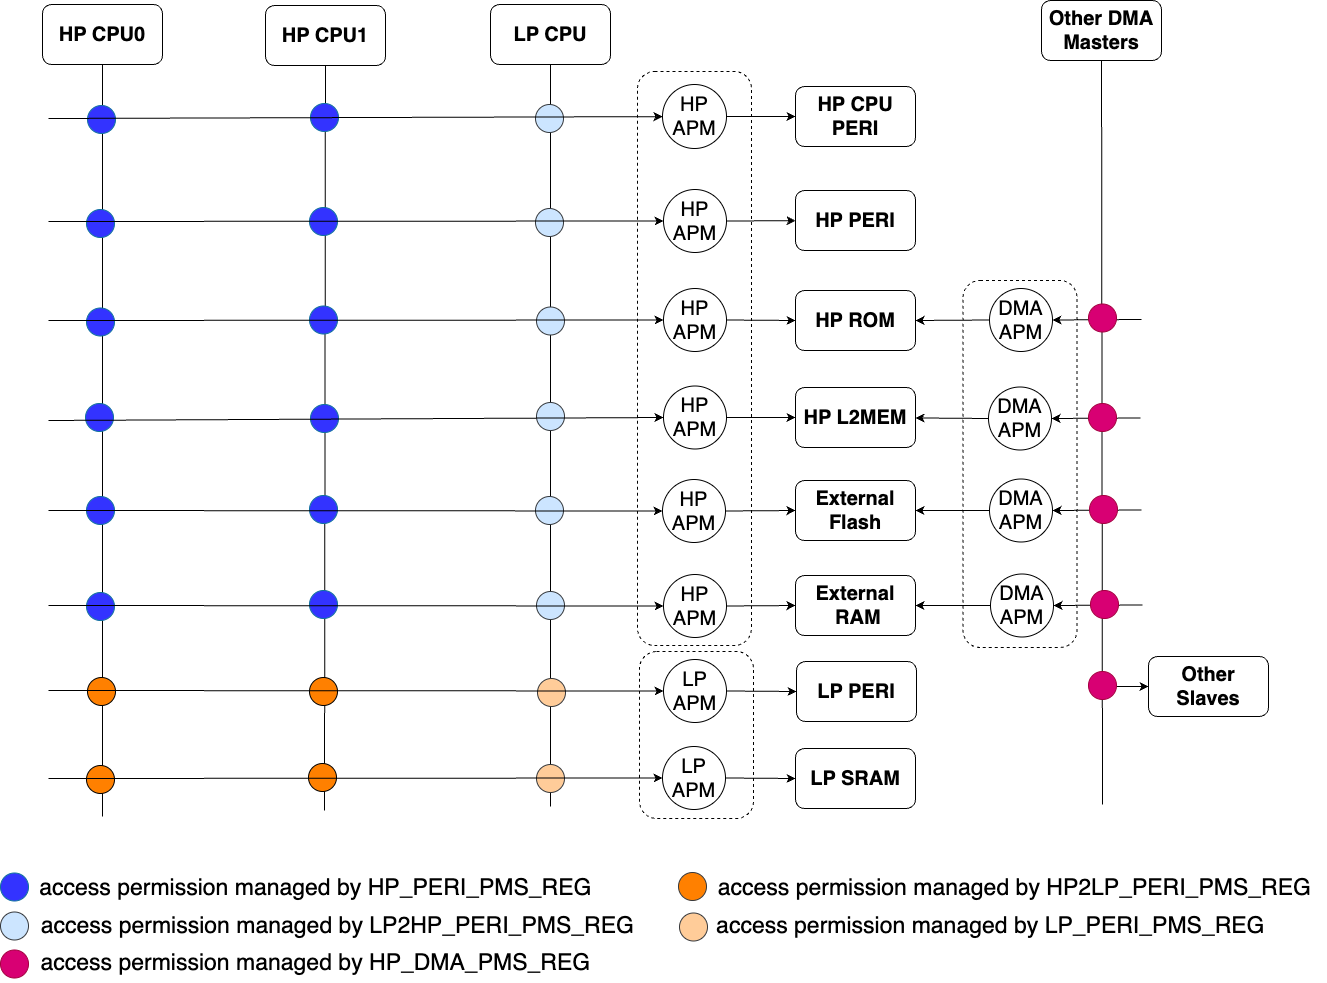
\includegraphics[width=1\linewidth]{21-PERMCTRL//figures/apm_architecture.png}
    \caption{APM 控制器结构图}
    \label{fig:APM_Ctrl_Location}
\end{figure}
\clearpage

\begin{tiplisting}
\vspace{-2em}
\begin{itemize}
    \item 寄存器名称“HP2LP”及“LP2HP”中的“HP”主要是指 HP CPU0/1，“LP”主要是指 LP CPU。
    \item 由表 \ref{tab:pmp-apm} 可知，HP CPU 和 LP CPU 访问 HP ROM、HP L2MEM、外部 flash 和 RAM 的地址空间不同。对于 HP CPU0/1，HP APM 管理的是 HP CPU0/1 不经过 cache 直接访问内存和外存的通路。
    \item \nameref{sec:permctrl-reg-lp} 中还额外包含了 \iftagged{ESP32-P4-latest}{8}{2} 个可配置地址区间及其对应的访问权限，可作用于 HP APM 和 LP APM，以管理全片外设寄存器（HP CPU PERI、HP PERI、LP PERI）的访问权限。
\end{itemize}
\end{tiplisting}

\subsection{地址区间及访问权限}
\label{sec:permctrl-addr-region}

APM 管理的地址区间分为固定地址区间和可配置地址区间。DMA APM 最多可管理 32 组可配置地址区间，HP APM 和 LP APM 除了控制固定地址区间外，还可管理 \iftagged{ESP32-P4-latest}{8}{2} 个可配置地址区间。

\subsubsection{HP APM 和 LP APM 管理的地址区间及访问权限}

HP APM 和 LP APM 控制的访问通路上，内部存储器和外部存储器通路采用固定地址区间管理访问权限，而全片外设寄存器通路上不仅支持固定地址区间的权限控制，还支持 \iftagged{ESP32-P4-latest}{8}{2} 个可配置地址区间。

\begin{itemize}
    \item 固定地址区间
    \begin{itemize}
        \item 固定地址区间即各个外设寄存器、内存和外存的有效地址空间。内存和外存地址空间见表 \ref{tab:pmp-apm}，各个外设寄存器的地址空间详见章节 \ref{mod:sysmem} \textit{\nameref{mod:sysmem}} > 表 \ref{tab:sysmem-base-address}。
        \item 要管理固定地址区间的访问权限，请参考图 \ref{fig:APM_Ctrl_Location} 确定访问通路及其对应的寄存器模块。
    \end{itemize}
    \item 可配置地址区间
    \begin{itemize}
        \item APM 可通过 \nameref{sec:permctrl-reg-lp} 中的 \hyperref[fielddesc:PMSPERIREGIONNLOW]{PMS\_PERI\_REGION\regindex{n}\tagged{ESP32-P4-latest}{/\regindex{m}}\_LOW\_REG} 和 \hyperref[fielddesc:PMSPERIREGIONNHIGH]{PMS\_PERI\_REGION\regindex{n}\tagged{ESP32-P4-latest}{/\regindex{m}}\_HIGH\_REG}（\regindex{n}\tagged{ESP32-P4-latest}{/\regindex{m}} = 0 \verb+~+ \iftagged{ESP32-P4-latest}{7}{1}) 配置 \iftagged{ESP32-P4-latest}{8}{2} 个地址区间，作用于 LP CPU 和 HP CPU0/1 到全片外设寄存器的访问通路。
        \item 可通过 \nameref{sec:permctrl-reg-lp} 中 \hyperref[regdesc:PMSPERIREGIONPMSREG]{PMS\_PERI\_REGION\_PMS\_REG} 管理可配置地址区间的访问权限。
    \end{itemize}
\end{itemize}

对全片外设寄存器访问进行访问权限管理时，可配置地址区间权限管理要先于固定地址区间权限管理，具体为：

\begin{itemize}
    \item 若访问地址在可配置地址区间内，则本次访问首先会接受可配置地址区间的检查。
    \begin{itemize}
        \item 如果有权限，则本次访问将继续接受后续固定地址区间的权限管理。
        \item 如果该访问没有权限，则访问被禁止，不会接受后续固定地址区间的权限管理。
    \end{itemize}
    \item 若访问地址在可配置地址区间之外，则本次访问直接跳过可配置地址区间检查，直接接受固定地址区间的权限管理。

    \item 可配置区间管理功能是对固定区间管理的补充。例如，配置了某固定地址区间的访问权限，将\tagged{ESP32-P4-latest}{其中} 2 个可配置地址区间限定在该固定地址区间内，并禁用其访问权限，便可实现在固定地址区间中设置 2 个禁止访问的地址区间。
\end{itemize}

\subsubsection{DMA APM 管理的地址区间及访问权限}

寄存器模块 \nameref{sec:permctrl-reg-dma} 中提供了 32 组可配置地址区间 (\hyperref[fielddesc:PMSDMAREGIONNLOW]{PMS\_DMA\_REGION\regindex{n}\_LOW\_REG} \verb+~+ \hyperref[fielddesc:PMSDMAREGIONNHIGH]{PMS\_DMA\_REGION\regindex{n}\_HIGH\_REG}, \regindex{n} = 0 \verb+~+ 31)，控制所有 DMA 主机的访问地址空间。配置该地址区间时，由于地址最小以 4K 字节对齐，故低 12 位为 0。

\nameref{sec:permctrl-reg-dma} 为每一个 DMA 主机访问每一个地址区间分配了独立的读权限和写权限。

\section{配置流程}

由于 HP CPU 有不同的工作模式（用户模式和机器模式），HP APM 和 LP APM 为不同工作模式分配了相应的访问管理权限。因此当 HP CPU 作为主机访问内存、外存或外设寄存器时，首先需要配置 HP CPU 的工作模式。

由于 LP CPU 仅支持机器模式，因此 HP APM 和 LP APM 仅为 LP CPU 的机器模式分配了访问权限位。

支持 DMA 传输的主设备不分访问模式，但 DMA APM 为 DMA 主设备分别提供了读和写操作管理权限。

\subsection{配置 HP CPU0/1 的访问权限}

HP CPU0/1 访问内存、外存或者外设寄存器路径中 APM 管控的配置流程为：

\begin{enumerate}
    \item 配置 HP CPU0/1 工作模式（用户模式或机器模式）。关于 CPU 用户模式及机器模式的配置方法请参考 RISC\-/V 指令集手册 v1.10 第二卷“特权架构” (RISC-V Instruction Set Manual, Volume II: Privileged Architecture, Version 1.10)。
    \item 如果访问外设寄存器，可额外管理 \iftagged{ESP32-P4-latest}{8}{2} 个可配置地址区间，请参考章节 \ref{sec:permctrl-addr-region}。
    \item 配置访问权限：
    \begin{itemize}
        \item 通过 \nameref{sec:permctrl-reg-hp} 配置 HP 系统一侧的内存（HP L2MEM 和 HP ROM）、外存（External RAM 和 flash）和外设寄存器（HP PERI 和 HP CPU PERI）的访问权限：
        \begin{itemize}
            \item 通过 \hyperref[fielddesc:PMSCORENMML2ROMALLOW]{PMS\_CORE\regindex{n}\_\regindex{MODE\_NAME}\_\regindex{MODULE\_NAME}\_ALLOW} 管理 HP CPU\regindex{n} 在 \regindex{MODE\_NAME} 模式下访问 \regindex{MODULE\_NAME} 模块的权限，比如 \hyperref[fielddesc:PMSCORENMMPSRAMALLOW]{PMS\_CORE\regindex{n}\_MM\_PSRAM\_ALLOW}。
        \end{itemize}
        \item 通过 \nameref{sec:permctrl-reg-hp2lp} 配置 LP SRAM 和 LP PERI 的访问权限：
            \begin{itemize}
            \item 通过 \hyperref[fielddesc:PMSHPCORENMMLPSYSREGALLOW]{PMS\_HP\_CORE\regindex{n}\_\regindex{MODE\_NAME}\_\regindex{MODULE\_NAME}\_ALLOW} 管理 HP CPU\regindex{n} 在 \regindex{MODE\_NAME} 模式下访问 \regindex{MODULE\_NAME} 模块的权限，比如 \hyperref[fielddesc:PMSHPCORENMMLPSYSREGALLOW]{PMS\_HP\_CORE\regindex{n}\_MM\_LP\_SYSREG\_ALLOW}。
        \end{itemize}
    \end{itemize}
\end{enumerate}

\subsection{配置 LP CPU 的访问权限}

LP CPU 仅支持机器模式，LP CPU 访问内存、外存或者外设寄存器路径中 APM 管控的配置流程为：

\begin{enumerate}
    \item 如果访问外设寄存器，可额外管理 \iftagged{ESP32-P4-latest}{8}{2} 个可配置地址区间，请参考章节 \ref{sec:permctrl-addr-region}。
    \item 配置访问权限：
    \begin{itemize}
        \item 通过 \nameref{sec:permctrl-reg-lp2hp} 配置 HP 系统一侧的内存（HP L2MEM 和 HP ROM）、外存（External RAM 和 flash）和外设寄存器（HP PERI 和 HP CPU PERI）的访问权限：
        \begin{itemize}
            \item 通过 \hyperref[fielddesc:PMSLPMML2ROMALLOW]{PMS\_LP\_MM\_\regindex{MODULE\_NAME}\_ALLOW} 管理 LP CPU 在机器模式下访问 \regindex{MODULE\_NAME} 模块的权限，比如 \hyperref[fielddesc:PMSLPMMPSRAMALLOW]{PMS\_LP\_MM\_PSRAM\_ALLOW}。
        \end{itemize}
        \item 通过 \nameref{sec:permctrl-reg-lp} 配置 LP 一侧的外设寄存器 (LP PERI) 的访问权限：
        \begin{itemize}
            \item 通过 \hyperref[fielddesc:PMSLPMMLPSYSREGALLOW]{PMS\_LP\_MM\_\regindex{MODULE\_NAME}\_ALLOW} 管理 LP CPU 在机器模式下访问 \regindex{MODULE\_NAME} 模块的权限，比如 \hyperref[fielddesc:PMSLPMMLPSYSREGALLOW]{PMS\_LP\_MM\_LP\_SYSREG\_ALLOW}。
        \end{itemize}
    \end{itemize}
\end{enumerate}

\subsection{配置其他 DMA 主机的访问权限}

DMA 主机访问内存、外存以及其它地址空间路径中 APM 管控的配置流程为：

\begin{enumerate}
    \item 配置所有 DMA 主机可访问的地址区间：
    \begin{itemize}
        \item 通过 \hyperref[regdesc:PMSDMAREGIONNLOWREG]{PMS\_DMA\_REGION\regindex{n}\_LOW\_REG} 配置 region\regindex{n} 的起始地址的高 20 位
        \item 通过 \hyperref[regdesc:PMSDMAREGIONNHIGHREG]{PMS\_DMA\_REGION\regindex{n}\_HIGH\_REG} 配置 region\regindex{n} 的结束地址的高 20 位
    \end{itemize}
    \item 配置每个 DMA 主机 (\regindex{DMA\_MASTER}) 各自访问每一个地址区间的读写权限：
    \begin{itemize}
        \item 通过 PMS\_\regindex{DMA\_MASTER}\_PMS\_R\_REG 配置读操作权限，如 \hyperref[regdesc:PMSDMAGMACPMSRREG]{PMS\_DMA\_GMAC\_PMS\_R\_REG}
        \item 通过 PMS\_\regindex{DMA\_MASTER}\_PMS\_W\_REG 配置写操作权限，如 \hyperref[regdesc:PMSDMAGMACPMSWREG]{PMS\_DMA\_GMAC\_PMS\_W\_REG}
    \end{itemize}
\end{enumerate}

\section{越权访问与中断}

APM 模块管理总线访问通路时，会解析总线携带的信息（主机 ID、访问方向、访问地址、甚至是运行模式)，然后根据此信息确定该访问的管理权限配置。当 APM 确认此次访问无权限时，\chipname{} 将视其为越权访问，将进行如下处理：

\begin{itemize}
    \item 拒绝该访问请求，并作错误响应
    \item HP APM  会触发 ICM\_SYS\_REG\_INT 中断信号
    \item DMA APM 会触发 ICM\_SYS\_REG\_INT 中断信号
    \item LP APM  会触发 LP\_SYSREG\_INT 中断信号
\end{itemize}

这些中断信号由 APM 管理模块的内部中断源生成。表 \ref{tab:apm-int-sources} 列出了 APM 管理模块的内部中断源、中断触发条件、以及生成的中断信号。

\begin{longtable}{ | l | L{8cm} | l | }
\caption{APM 内部中断源} \label{tab:apm-int-sources}
\\ \hline
\rowcolor{lightgray}
\textbf{内部中断源} & \textbf{触发条件}  &  \textbf{中断信号}\\ \hline
ICM\_CPU\_ADDRHOLE\_INTR &  HP APM 检测到越权访问；或当主机为高速 USB 2.0 OTG、全速 USB 2.0 OTG、EMAC、SDMMC、Trace0/1、GDMA-AHB、L2MEM 监测器和 SPM 监测器时，DMA APM 检测到越权访问 &  ICM\_SYS\_REG\_INT \\ \hline
ICM\_SYS\_ADDRHOLE\_INTR & 当主机为 VDMA、GDMA-AXI、2D-DMA 和 H264 DMA 时 DMA APM 发生了越权访问 &  ICM\_SYS\_REG\_INT \\ \hline
LP\_ADDRHOLE\_INTR &  LP APM 检测到越权访问 &  LP\_SYSREG\_INTR  \\ \hline
\end{longtable}

APM 会自动记录非法访问的相关信息，包括主机 ID、访问方向（读或者写）、访问地址、非法访问标志等信息。所有这些信息可以从章节 \ref{mod:sysreg} \textit{\nameref{mod:sysreg}} 中的相关寄存器中获取。

% >>> If your module has no registers, delete sample text
%       for Sections Register Summary and Registers below <<<

%%%%%%%%%%%%%%%%%%%%%%%%
%%% Register Summary %%%
%%%%%%%%%%%%%%%%%%%%%%%%

% >>> Update the sample text below and insert
%     the info on register summary into the subfile <<<

\clearpage
\hypertarget{permctrl-reg-summ}{}
\section{寄存器列表}
\label{sec:permctrl-reg-summ}

\subsection{HP\_DMA\_PMS\_REG}
\label{sec:permctrl-reg-dma}

本小节的所有地址均为相对于 HP\_DMA\_PMS 基地址的地址偏移量（相对地址），具体基地址请见章节 \ref{mod:sysmem} \textit{\nameref{mod:sysmem}} 中的表 \ref{tab:sysmem-base-address}。

请查看章节 \hyperref[glossary-access-types]{\textit{寄存器的访问类型}}，了解“访问”列缩写的含义。
\begin{longtable}{ | L{7.5cm} | L{6cm} | L{1.3cm} | L{1cm} | }
\hline\rowcolor{lightgray}
\textbf{名称} & \textbf{描述} &  \textbf{地址} & \textbf{访问} \\ \hline
\endhead
\multicolumn{4}{|l|}{\textbf{版本控制寄存器}} \\ \hline
\hyperref[regdesc:PMSDMADATEREG]{PMS\_DMA\_DATE\_REG} & 版本控制寄存器 & 0x0000 & R/W \\ \hline
\multicolumn{4}{|l|}{\textbf{时钟门控寄存器}} \\ \hline
\hyperref[regdesc:PMSDMACLKENREG]{PMS\_DMA\_CLK\_EN\_REG} & 时钟门控寄存器 & 0x0004 & R/W \\ \hline
\multicolumn{4}{|l|}{\textbf{地址区间配置寄存器}} \\ \hline
\hyperref[regdesc:PMSDMAREGIONNLOWREG]{PMS\_DMA\_REGION0\_LOW\_REG} & 地址区间 0 起始地址配置寄存器 & 0x0008 & R/W \\ \hline
\hyperref[regdesc:PMSDMAREGIONNHIGHREG]{PMS\_DMA\_REGION0\_HIGH\_REG} & 地址区间 0 结束地址配置寄存器 & 0x000C & R/W \\ \hline
\hyperref[regdesc:PMSDMAREGIONNLOWREG]{PMS\_DMA\_REGION1\_LOW\_REG} & 地址区间 1 起始地址配置寄存器 & 0x0010 & R/W \\ \hline
\hyperref[regdesc:PMSDMAREGIONNHIGHREG]{PMS\_DMA\_REGION1\_HIGH\_REG} & 地址区间 1 结束地址配置寄存器 & 0x0014 & R/W \\ \hline
\hyperref[regdesc:PMSDMAREGIONNLOWREG]{PMS\_DMA\_REGION2\_LOW\_REG} & 地址区间 2 起始地址配置寄存器 & 0x0018 & R/W \\ \hline
\hyperref[regdesc:PMSDMAREGIONNHIGHREG]{PMS\_DMA\_REGION2\_HIGH\_REG} & 地址区间 2 结束地址配置寄存器 & 0x001C & R/W \\ \hline
\hyperref[regdesc:PMSDMAREGIONNLOWREG]{PMS\_DMA\_REGION3\_LOW\_REG} & 地址区间 3 起始地址配置寄存器 & 0x0020 & R/W \\ \hline
\hyperref[regdesc:PMSDMAREGIONNHIGHREG]{PMS\_DMA\_REGION3\_HIGH\_REG} & 地址区间 3 结束地址配置寄存器 & 0x0024 & R/W \\ \hline
\hyperref[regdesc:PMSDMAREGIONNLOWREG]{PMS\_DMA\_REGION4\_LOW\_REG} & 地址区间 4 起始地址配置寄存器 & 0x0028 & R/W \\ \hline
\hyperref[regdesc:PMSDMAREGIONNHIGHREG]{PMS\_DMA\_REGION4\_HIGH\_REG} & 地址区间 4 结束地址配置寄存器 & 0x002C & R/W \\ \hline
\hyperref[regdesc:PMSDMAREGIONNLOWREG]{PMS\_DMA\_REGION5\_LOW\_REG} & 地址区间 5 起始地址配置寄存器 & 0x0030 & R/W \\ \hline
\hyperref[regdesc:PMSDMAREGIONNHIGHREG]{PMS\_DMA\_REGION5\_HIGH\_REG} & 地址区间 5 结束地址配置寄存器 & 0x0034 & R/W \\ \hline
\hyperref[regdesc:PMSDMAREGIONNLOWREG]{PMS\_DMA\_REGION6\_LOW\_REG} & 地址区间 6 起始地址配置寄存器 & 0x0038 & R/W \\ \hline
\hyperref[regdesc:PMSDMAREGIONNHIGHREG]{PMS\_DMA\_REGION6\_HIGH\_REG} & 地址区间 6 结束地址配置寄存器 & 0x003C & R/W \\ \hline
\hyperref[regdesc:PMSDMAREGIONNLOWREG]{PMS\_DMA\_REGION7\_LOW\_REG} & 地址区间 7 起始地址配置寄存器 & 0x0040 & R/W \\ \hline
\hyperref[regdesc:PMSDMAREGIONNHIGHREG]{PMS\_DMA\_REGION7\_HIGH\_REG} & 地址区间 7 结束地址配置寄存器 & 0x0044 & R/W \\ \hline
\hyperref[regdesc:PMSDMAREGIONNLOWREG]{PMS\_DMA\_REGION8\_LOW\_REG} & 地址区间 8 起始地址配置寄存器 & 0x0048 & R/W \\ \hline
\hyperref[regdesc:PMSDMAREGIONNHIGHREG]{PMS\_DMA\_REGION8\_HIGH\_REG} & 地址区间 8 结束地址配置寄存器 & 0x004C & R/W \\ \hline
\hyperref[regdesc:PMSDMAREGIONNLOWREG]{PMS\_DMA\_REGION9\_LOW\_REG} & 地址区间 9 起始地址配置寄存器 & 0x0050 & R/W \\ \hline
\hyperref[regdesc:PMSDMAREGIONNHIGHREG]{PMS\_DMA\_REGION9\_HIGH\_REG} & 地址区间 9 结束地址配置寄存器 & 0x0054 & R/W \\ \hline
\hyperref[regdesc:PMSDMAREGIONNLOWREG]{PMS\_DMA\_REGION10\_LOW\_REG} & 地址区间 10 起始地址配置寄存器 & 0x0058 & R/W \\ \hline
\hyperref[regdesc:PMSDMAREGIONNHIGHREG]{PMS\_DMA\_REGION10\_HIGH\_REG} & 地址区间 10 结束地址配置寄存器 & 0x005C & R/W \\ \hline
\hyperref[regdesc:PMSDMAREGIONNLOWREG]{PMS\_DMA\_REGION11\_LOW\_REG} & 地址区间 11 起始地址配置寄存器 & 0x0060 & R/W \\ \hline
\hyperref[regdesc:PMSDMAREGIONNHIGHREG]{PMS\_DMA\_REGION11\_HIGH\_REG} & 地址区间 11 结束地址配置寄存器 & 0x0064 & R/W \\ \hline
\hyperref[regdesc:PMSDMAREGIONNLOWREG]{PMS\_DMA\_REGION12\_LOW\_REG} & 地址区间 12 起始地址配置寄存器 & 0x0068 & R/W \\ \hline
\hyperref[regdesc:PMSDMAREGIONNHIGHREG]{PMS\_DMA\_REGION12\_HIGH\_REG} & 地址区间 12 结束地址配置寄存器 & 0x006C & R/W \\ \hline
\hyperref[regdesc:PMSDMAREGIONNLOWREG]{PMS\_DMA\_REGION13\_LOW\_REG} & 地址区间 13 起始地址配置寄存器 & 0x0070 & R/W \\ \hline
\hyperref[regdesc:PMSDMAREGIONNHIGHREG]{PMS\_DMA\_REGION13\_HIGH\_REG} & 地址区间 13 结束地址配置寄存器 & 0x0074 & R/W \\ \hline
\hyperref[regdesc:PMSDMAREGIONNLOWREG]{PMS\_DMA\_REGION14\_LOW\_REG} & 地址区间 14 起始地址配置寄存器 & 0x0078 & R/W \\ \hline
\hyperref[regdesc:PMSDMAREGIONNHIGHREG]{PMS\_DMA\_REGION14\_HIGH\_REG} & 地址区间 14 结束地址配置寄存器 & 0x007C & R/W \\ \hline
\hyperref[regdesc:PMSDMAREGIONNLOWREG]{PMS\_DMA\_REGION15\_LOW\_REG} & 地址区间 15 起始地址配置寄存器 & 0x0080 & R/W \\ \hline
\hyperref[regdesc:PMSDMAREGIONNHIGHREG]{PMS\_DMA\_REGION15\_HIGH\_REG} & 地址区间 15 结束地址配置寄存器 & 0x0084 & R/W \\ \hline
\hyperref[regdesc:PMSDMAREGIONNLOWREG]{PMS\_DMA\_REGION16\_LOW\_REG} & 地址区间 16 起始地址配置寄存器 & 0x0088 & R/W \\ \hline
\hyperref[regdesc:PMSDMAREGIONNHIGHREG]{PMS\_DMA\_REGION16\_HIGH\_REG} & 地址区间 16 结束地址配置寄存器 & 0x008C & R/W \\ \hline
\hyperref[regdesc:PMSDMAREGIONNLOWREG]{PMS\_DMA\_REGION17\_LOW\_REG} & 地址区间 17 起始地址配置寄存器 & 0x0090 & R/W \\ \hline
\hyperref[regdesc:PMSDMAREGIONNHIGHREG]{PMS\_DMA\_REGION17\_HIGH\_REG} & 地址区间 17 结束地址配置寄存器 & 0x0094 & R/W \\ \hline
\hyperref[regdesc:PMSDMAREGIONNLOWREG]{PMS\_DMA\_REGION18\_LOW\_REG} & 地址区间 18 起始地址配置寄存器 & 0x0098 & R/W \\ \hline
\hyperref[regdesc:PMSDMAREGIONNHIGHREG]{PMS\_DMA\_REGION18\_HIGH\_REG} & 地址区间 18 结束地址配置寄存器 & 0x009C & R/W \\ \hline
\hyperref[regdesc:PMSDMAREGIONNLOWREG]{PMS\_DMA\_REGION19\_LOW\_REG} & 地址区间 19 起始地址配置寄存器 & 0x00A0 & R/W \\ \hline
\hyperref[regdesc:PMSDMAREGIONNHIGHREG]{PMS\_DMA\_REGION19\_HIGH\_REG} & 地址区间 19 结束地址配置寄存器 & 0x00A4 & R/W \\ \hline
\hyperref[regdesc:PMSDMAREGIONNLOWREG]{PMS\_DMA\_REGION20\_LOW\_REG} & 地址区间 20 起始地址配置寄存器 & 0x00A8 & R/W \\ \hline
\hyperref[regdesc:PMSDMAREGIONNHIGHREG]{PMS\_DMA\_REGION20\_HIGH\_REG} & 地址区间 20 结束地址配置寄存器 & 0x00AC & R/W \\ \hline
\hyperref[regdesc:PMSDMAREGIONNLOWREG]{PMS\_DMA\_REGION21\_LOW\_REG} & 地址区间 21 起始地址配置寄存器 & 0x00B0 & R/W \\ \hline
\hyperref[regdesc:PMSDMAREGIONNHIGHREG]{PMS\_DMA\_REGION21\_HIGH\_REG} & 地址区间 21 结束地址配置寄存器 & 0x00B4 & R/W \\ \hline
\hyperref[regdesc:PMSDMAREGIONNLOWREG]{PMS\_DMA\_REGION22\_LOW\_REG} & 地址区间 22 起始地址配置寄存器 & 0x00B8 & R/W \\ \hline
\hyperref[regdesc:PMSDMAREGIONNHIGHREG]{PMS\_DMA\_REGION22\_HIGH\_REG} & 地址区间 22 结束地址配置寄存器 & 0x00BC & R/W \\ \hline
\hyperref[regdesc:PMSDMAREGIONNLOWREG]{PMS\_DMA\_REGION23\_LOW\_REG} & 地址区间 23 起始地址配置寄存器 & 0x00C0 & R/W \\ \hline
\hyperref[regdesc:PMSDMAREGIONNHIGHREG]{PMS\_DMA\_REGION23\_HIGH\_REG} & 地址区间 23 结束地址配置寄存器 & 0x00C4 & R/W \\ \hline
\hyperref[regdesc:PMSDMAREGIONNLOWREG]{PMS\_DMA\_REGION24\_LOW\_REG} & 地址区间 24 起始地址配置寄存器 & 0x00C8 & R/W \\ \hline
\hyperref[regdesc:PMSDMAREGIONNHIGHREG]{PMS\_DMA\_REGION24\_HIGH\_REG} & 地址区间 24 结束地址配置寄存器 & 0x00CC & R/W \\ \hline
\hyperref[regdesc:PMSDMAREGIONNLOWREG]{PMS\_DMA\_REGION25\_LOW\_REG} & 地址区间 25 起始地址配置寄存器 & 0x00D0 & R/W \\ \hline
\hyperref[regdesc:PMSDMAREGIONNHIGHREG]{PMS\_DMA\_REGION25\_HIGH\_REG} & 地址区间 25 结束地址配置寄存器 & 0x00D4 & R/W \\ \hline
\hyperref[regdesc:PMSDMAREGIONNLOWREG]{PMS\_DMA\_REGION26\_LOW\_REG} & 地址区间 26 起始地址配置寄存器 & 0x00D8 & R/W \\ \hline
\hyperref[regdesc:PMSDMAREGIONNHIGHREG]{PMS\_DMA\_REGION26\_HIGH\_REG} & 地址区间 26 结束地址配置寄存器 & 0x00DC & R/W \\ \hline
\hyperref[regdesc:PMSDMAREGIONNLOWREG]{PMS\_DMA\_REGION27\_LOW\_REG} & 地址区间 27 起始地址配置寄存器 & 0x00E0 & R/W \\ \hline
\hyperref[regdesc:PMSDMAREGIONNHIGHREG]{PMS\_DMA\_REGION27\_HIGH\_REG} & 地址区间 27 结束地址配置寄存器 & 0x00E4 & R/W \\ \hline
\hyperref[regdesc:PMSDMAREGIONNLOWREG]{PMS\_DMA\_REGION28\_LOW\_REG} & 地址区间 28 起始地址配置寄存器 & 0x00E8 & R/W \\ \hline
\hyperref[regdesc:PMSDMAREGIONNHIGHREG]{PMS\_DMA\_REGION28\_HIGH\_REG} & 地址区间 28 结束地址配置寄存器 & 0x00EC & R/W \\ \hline
\hyperref[regdesc:PMSDMAREGIONNLOWREG]{PMS\_DMA\_REGION29\_LOW\_REG} & 地址区间 29 起始地址配置寄存器 & 0x00F0 & R/W \\ \hline
\hyperref[regdesc:PMSDMAREGIONNHIGHREG]{PMS\_DMA\_REGION29\_HIGH\_REG} & 地址区间 29 结束地址配置寄存器 & 0x00F4 & R/W \\ \hline
\hyperref[regdesc:PMSDMAREGIONNLOWREG]{PMS\_DMA\_REGION30\_LOW\_REG} & 地址区间 30 起始地址配置寄存器 & 0x00F8 & R/W \\ \hline
\hyperref[regdesc:PMSDMAREGIONNHIGHREG]{PMS\_DMA\_REGION30\_HIGH\_REG} & 地址区间 30 结束地址配置寄存器 & 0x00FC & R/W \\ \hline
\hyperref[regdesc:PMSDMAREGIONNLOWREG]{PMS\_DMA\_REGION31\_LOW\_REG} & 地址区间 31 起始地址配置寄存器 & 0x0100 & R/W \\ \hline
\hyperref[regdesc:PMSDMAREGIONNHIGHREG]{PMS\_DMA\_REGION31\_HIGH\_REG} & 地址区间 31 结束地址配置寄存器 & 0x0104 & R/W \\ \hline
\multicolumn{4}{|l|}{\textbf{DMA 主机读写权限配置寄存器}} \\ \hline
\hyperref[regdesc:PMSDMAGDMACHNRPMSREG]{PMS\_DMA\_GDMA\_CH0\_R\_PMS\_REG} & GDMA ch0 读权限控制寄存器 & 0x0108 & R/W \\ \hline
\hyperref[regdesc:PMSDMAGDMACHNWPMSREG]{PMS\_DMA\_GDMA\_CH0\_W\_PMS\_REG} & GDMA ch0 写权限控制寄存器 & 0x010C & R/W \\ \hline
\hyperref[regdesc:PMSDMAGDMACHNRPMSREG]{PMS\_DMA\_GDMA\_CH1\_R\_PMS\_REG} & GDMA ch1 读权限控制寄存器 & 0x0110 & R/W \\ \hline
\hyperref[regdesc:PMSDMAGDMACHNWPMSREG]{PMS\_DMA\_GDMA\_CH1\_W\_PMS\_REG} & GDMA ch1 写权限控制寄存器 & 0x0114 & R/W \\ \hline
\hyperref[regdesc:PMSDMAGDMACHNRPMSREG]{PMS\_DMA\_GDMA\_CH2\_R\_PMS\_REG} & GDMA ch2 读权限控制寄存器 & 0x0118 & R/W \\ \hline
\hyperref[regdesc:PMSDMAGDMACHNWPMSREG]{PMS\_DMA\_GDMA\_CH2\_W\_PMS\_REG} & GDMA ch2 写权限控制寄存器 & 0x011C & R/W \\ \hline
\hyperref[regdesc:PMSDMAGDMACHNRPMSREG]{PMS\_DMA\_GDMA\_CH3\_R\_PMS\_REG} & GDMA ch3 读权限控制寄存器 & 0x0120 & R/W \\ \hline
\hyperref[regdesc:PMSDMAGDMACHNWPMSREG]{PMS\_DMA\_GDMA\_CH3\_W\_PMS\_REG} & GDMA ch3 写权限控制寄存器 & 0x0124 & R/W \\ \hline
\hyperref[regdesc:PMSDMAAHBPDMAADCRPMSREG]{PMS\_DMA\_AHB\_PDMA\_ADC\_R\_PMS\_REG} & GDMA-AHB ADC 读权限控制寄存器 & 0x0128 & R/W \\ \hline
\hyperref[regdesc:PMSDMAAHBPDMAADCWPMSREG]{PMS\_DMA\_AHB\_PDMA\_ADC\_W\_PMS\_REG} & GDMA-AHB ADC 写权限控制寄存器 & 0x012C & R/W \\ \hline
\hyperref[regdesc:PMSDMAAHBPDMAI2S0RPMSREG]{PMS\_DMA\_AHB\_PDMA\_I2S0\_R\_PMS\_REG} & GDMA-AHB I2S0 读权限控制寄存器 & 0x0130 & R/W \\ \hline
\hyperref[regdesc:PMSDMAAHBPDMAI2S0WPMSREG]{PMS\_DMA\_AHB\_PDMA\_I2S0\_W\_PMS\_REG} & GDMA-AHB I2S0 写权限控制寄存器 & 0x0134 & R/W \\ \hline
\hyperref[regdesc:PMSDMAAHBPDMAI2S1RPMSREG]{PMS\_DMA\_AHB\_PDMA\_I2S1\_R\_PMS\_REG} & GDMA-AHB I2S1 读权限控制寄存器 & 0x0138 & R/W \\ \hline
\hyperref[regdesc:PMSDMAAHBPDMAI2S1WPMSREG]{PMS\_DMA\_AHB\_PDMA\_I2S1\_W\_PMS\_REG} & GDMA-AHB I2S1 写权限控制寄存器 & 0x013C & R/W \\ \hline
\hyperref[regdesc:PMSDMAAHBPDMAI2S2RPMSREG]{PMS\_DMA\_AHB\_PDMA\_I2S2\_R\_PMS\_REG} & GDMA-AHB I2S2 读权限控制寄存器 & 0x0140 & R/W \\ \hline
\hyperref[regdesc:PMSDMAAHBPDMAI2S2WPMSREG]{PMS\_DMA\_AHB\_PDMA\_I2S2\_W\_PMS\_REG} & GDMA-AHB I2S2 写权限控制寄存器 & 0x0144 & R/W \\ \hline
\hyperref[regdesc:PMSDMAAHBPDMAI3CMSTRPMSREG]{PMS\_DMA\_AHB\_PDMA\_I3C\_MST\_R\_PMS\_REG} & GDMA-AHB I3C MST 读权限控制寄存器 & 0x0148 & R/W \\ \hline
\hyperref[regdesc:PMSDMAAHBPDMAI3CMSTWPMSREG]{PMS\_DMA\_AHB\_PDMA\_I3C\_MST\_W\_PMS\_REG} & GDMA-AHB I3C MST 写权限控制寄存器 & 0x014C & R/W \\ \hline
\hyperref[regdesc:PMSDMAAHBPDMAUHCI0RPMSREG]{PMS\_DMA\_AHB\_PDMA\_UHCI0\_R\_PMS\_REG} & GDMA-AHB UHCI 读权限控制寄存器 & 0x0150 & R/W \\ \hline
\hyperref[regdesc:PMSDMAAHBPDMAUHCI0WPMSREG]{PMS\_DMA\_AHB\_PDMA\_UHCI0\_W\_PMS\_REG} & GDMA-AHB UHCI 写权限控制寄存器 & 0x0154 & R/W \\ \hline
\hyperref[regdesc:PMSDMAAHBPDMARMTRPMSREG]{PMS\_DMA\_AHB\_PDMA\_RMT\_R\_PMS\_REG} & GDMA-AHB RMT 读权限控制寄存器 & 0x0158 & R/W \\ \hline
\hyperref[regdesc:PMSDMAAHBPDMARMTWPMSREG]{PMS\_DMA\_AHB\_PDMA\_RMT\_W\_PMS\_REG} & GDMA-AHB RMT 写权限控制寄存器 & 0x0170 & R/W \\ \hline
\hyperref[regdesc:PMSDMAAXIPDMALCDCAMRPMSREG]{PMS\_DMA\_AXI\_PDMA\_LCDCAM\_R\_PMS\_REG} & GDMA-AXI LCDCAM 读权限控制寄存器 & 0x0174 & R/W \\ \hline
\hyperref[regdesc:PMSDMAAXIPDMALCDCAMWPMSREG]{PMS\_DMA\_AXI\_PDMA\_LCDCAM\_W\_PMS\_REG} & GDMA-AXI LCDCAM 写权限控制寄存器 & 0x0178 & R/W \\ \hline
\hyperref[regdesc:PMSDMAAXIPDMAGPSPI2RPMSREG]{PMS\_DMA\_AXI\_PDMA\_GPSPI2\_R\_PMS\_REG} & GDMA-AXI GP-SPI2 读权限控制寄存器 & 0x017C & R/W \\ \hline
\hyperref[regdesc:PMSDMAAXIPDMAGPSPI2WPMSREG]{PMS\_DMA\_AXI\_PDMA\_GPSPI2\_W\_PMS\_REG} & GDMA-AXI GP-SPI2 写权限控制寄存器 & 0x0180 & R/W \\ \hline
\hyperref[regdesc:PMSDMAAXIPDMAGPSPI3RPMSREG]{PMS\_DMA\_AXI\_PDMA\_GPSPI3\_R\_PMS\_REG} & GDMA-AXI GP-SPI3 读权限控制寄存器 & 0x0184 & R/W \\ \hline
\hyperref[regdesc:PMSDMAAXIPDMAGPSPI3WPMSREG]{PMS\_DMA\_AXI\_PDMA\_GPSPI3\_W\_PMS\_REG} & GDMA-AXI GP-SPI3 写权限控制寄存器 & 0x0188 & R/W \\ \hline
\hyperref[regdesc:PMSDMAAXIPDMAPARLIORPMSREG]{PMS\_DMA\_AXI\_PDMA\_PARLIO\_R\_PMS\_REG} & GDMA-AXI PARLIO 读权限控制寄存器 & 0x018C & R/W \\ \hline
\hyperref[regdesc:PMSDMAAXIPDMAPARLIOWPMSREG]{PMS\_DMA\_AXI\_PDMA\_PARLIO\_W\_PMS\_REG} & GDMA-AXI PARLIO 写权限控制寄存器 & 0x0190 & R/W \\ \hline
\hyperref[regdesc:PMSDMAAXIPDMAAESRPMSREG]{PMS\_DMA\_AXI\_PDMA\_AES\_R\_PMS\_REG} & GDMA-AXI AES 读权限控制寄存器 & 0x0194 & R/W \\ \hline
\hyperref[regdesc:PMSDMAAXIPDMAAESWPMSREG]{PMS\_DMA\_AXI\_PDMA\_AES\_W\_PMS\_REG} & GDMA-AXI AES 写权限控制寄存器 & 0x0198 & R/W \\ \hline
\hyperref[regdesc:PMSDMAAXIPDMASHARPMSREG]{PMS\_DMA\_AXI\_PDMA\_SHA\_R\_PMS\_REG} & GDMA-AXI SHA 读权限控制寄存器 & 0x019C & R/W \\ \hline
\hyperref[regdesc:PMSDMAAXIPDMASHAWPMSREG]{PMS\_DMA\_AXI\_PDMA\_SHA\_W\_PMS\_REG} & GDMA-AXI SHA 写权限控制寄存器 & 0x01A0 & R/W \\ \hline
\hyperref[regdesc:PMSDMADMA2DJPEGPMSRREG]{PMS\_DMA\_DMA2D\_JPEG\_PMS\_R\_REG} & 2D-DMA JPEG 读权限控制寄存器 & 0x01A4 & R/W \\ \hline
\hyperref[regdesc:PMSDMADMA2DJPEGPMSWREG]{PMS\_DMA\_DMA2D\_JPEG\_PMS\_W\_REG} & 2D-DMA JPEG 写权限控制寄存器 & 0x01A8 & R/W \\ \hline
\hyperref[regdesc:PMSDMAUSBPMSRREG]{PMS\_DMA\_USB\_PMS\_R\_REG} & 高速 USB 2.0 OTG 读权限控制寄存器 & 0x01AC & R/W \\ \hline
\hyperref[regdesc:PMSDMAUSBPMSWREG]{PMS\_DMA\_USB\_PMS\_W\_REG} & 高速 USB 2.0 OTG 写权限控制寄存器 & 0x01B0 & R/W \\ \hline
\hyperref[regdesc:PMSDMAGMACPMSRREG]{PMS\_DMA\_GMAC\_PMS\_R\_REG} & EMAC 读权限控制寄存器 & 0x01B4 & R/W \\ \hline
\hyperref[regdesc:PMSDMAGMACPMSWREG]{PMS\_DMA\_GMAC\_PMS\_W\_REG} & EMAC 写权限控制寄存器 & 0x01B8 & R/W \\ \hline
\hyperref[regdesc:PMSDMASDMMCPMSRREG]{PMS\_DMA\_SDMMC\_PMS\_R\_REG} & SDMMC 读权限控制寄存器 & 0x01BC & R/W \\ \hline
\hyperref[regdesc:PMSDMASDMMCPMSWREG]{PMS\_DMA\_SDMMC\_PMS\_W\_REG} & SDMMC 写权限控制寄存器 & 0x01C0 & R/W \\ \hline
\hyperref[regdesc:PMSDMAUSBOTG11PMSRREG]{PMS\_DMA\_USBOTG11\_PMS\_R\_REG} & 全速 USB 2.0 OTG 读权限控制寄存器 & 0x01C4 & R/W \\ \hline
\hyperref[regdesc:PMSDMAUSBOTG11PMSWREG]{PMS\_DMA\_USBOTG11\_PMS\_W\_REG} & 全速 USB 2.0 OTG 写权限控制寄存器 & 0x01C8 & R/W \\ \hline
\hyperref[regdesc:PMSDMATRACE0PMSRREG]{PMS\_DMA\_TRACE0\_PMS\_R\_REG} & TRACE0 读权限控制寄存器 & 0x01CC & R/W \\ \hline
\hyperref[regdesc:PMSDMATRACE0PMSWREG]{PMS\_DMA\_TRACE0\_PMS\_W\_REG} & TRACE0 写权限控制寄存器 & 0x01D0 & R/W \\ \hline
\hyperref[regdesc:PMSDMATRACE1PMSRREG]{PMS\_DMA\_TRACE1\_PMS\_R\_REG} & TRACE1 读权限控制寄存器 & 0x01D4 & R/W \\ \hline
\hyperref[regdesc:PMSDMATRACE1PMSWREG]{PMS\_DMA\_TRACE1\_PMS\_W\_REG} & TRACE1 写权限控制寄存器 & 0x01D8 & R/W \\ \hline
\hyperref[regdesc:PMSDMAL2MEMMONPMSWREG]{PMS\_DMA\_L2MEM\_MON\_PMS\_W\_REG} & L2MEM 监测器写权限控制寄存器 & 0x01E0 & R/W \\ \hline
\hyperref[regdesc:PMSDMASPMMONPMSWREG]{PMS\_DMA\_SPM\_MON\_PMS\_W\_REG} & SPM 监测器写权限控制寄存器 & 0x01E8 & R/W \\ \hline
\hyperref[regdesc:PMSDMAH264PMSRREG]{PMS\_DMA\_H264\_PMS\_R\_REG} & H264 DMA 读权限控制寄存器 & 0x01FC & R/W \\ \hline
\hyperref[regdesc:PMSDMAH264PMSWREG]{PMS\_DMA\_H264\_PMS\_W\_REG} & H264 DMA 写权限控制寄存器 & 0x0200 & R/W \\ \hline
\hyperref[regdesc:PMSDMADMA2DPPAPMSRREG]{PMS\_DMA\_DMA2D\_PPA\_PMS\_R\_REG} & 2D-DMA PPA 读权限控制寄存器 & 0x0204 & R/W \\ \hline
\hyperref[regdesc:PMSDMADMA2DPPAPMSWREG]{PMS\_DMA\_DMA2D\_PPA\_PMS\_W\_REG} & 2D-DMA PPA 写权限控制寄存器 & 0x0208 & R/W \\ \hline
\hyperref[regdesc:PMSDMADMA2DDUMMYPMSRREG]{PMS\_DMA\_DMA2D\_DUMMY\_PMS\_R\_REG} & 2D-DMA Dummy 读权限控制寄存器 & 0x020C & R/W \\ \hline
\hyperref[regdesc:PMSDMADMA2DDUMMYPMSWREG]{PMS\_DMA\_DMA2D\_DUMMY\_PMS\_W\_REG} & 2D-DMA Dummy 写权限控制寄存器 & 0x0210 & R/W \\ \hline
\hyperref[regdesc:PMSDMAAHBPDMADUMMYRPMSREG]{PMS\_DMA\_AHB\_PDMA\_DUMMY\_R\_PMS\_REG} & GDMA-AHB Dummy 读权限控制寄存器 & 0x0214 & R/W \\ \hline
\hyperref[regdesc:PMSDMAAHBPDMADUMMYWPMSREG]{PMS\_DMA\_AHB\_PDMA\_DUMMY\_W\_PMS\_REG} & GDMA-AHB Dummy 写权限控制寄存器 & 0x0218 & R/W \\ \hline
\hyperref[regdesc:PMSDMAAXIPDMADUMMYRPMSREG]{PMS\_DMA\_AXI\_PDMA\_DUMMY\_R\_PMS\_REG} & GDMA-AXI Dummy 读权限控制寄存器 & 0x021C & R/W \\ \hline
\hyperref[regdesc:PMSDMAAXIPDMADUMMYWPMSREG]{PMS\_DMA\_AXI\_PDMA\_DUMMY\_W\_PMS\_REG} & GDMA-AXI Dummy 写权限控制寄存器 & 0x0220 & R/W \\ \hline
\end{longtable}


\subsection{HP\_PERI\_PMS\_REG}
\label{sec:permctrl-reg-hp}

本小节的所有地址均为相对于 HP\_PERI\_PMS 基地址的地址偏移量（相对地址），具体基地址请见章节 \ref{mod:sysmem} \textit{\nameref{mod:sysmem}} 中的表 \ref{tab:sysmem-base-address}。

请查看章节 \hyperref[glossary-access-types]{\textit{寄存器的访问类型}}，了解“访问”列缩写的含义。
\begin{longtable}{ | L{7.2cm} | L{6cm} | L{1.3cm} | L{1cm} | }
\hline\rowcolor{lightgray}
\textbf{名称} & \textbf{描述} &  \textbf{地址} & \textbf{访问}\\ \hline
\endhead
\multicolumn{4}{|l|}{\textbf{版本控制寄存器}} \\ \hline
\hyperref[regdesc:PMSHPPERIPMSDATEREG]{PMS\_HP\_PERI\_PMS\_DATE\_REG} & 版本控制寄存器 & 0x0000 & R/W \\ \hline
\multicolumn{4}{|l|}{\textbf{时钟门控寄存器}} \\ \hline
\hyperref[regdesc:PMSHPPERIPMSCLKENREG]{PMS\_HP\_PERI\_PMS\_CLK\_EN\_REG} & 时钟门控寄存器 & 0x0004 & R/W \\ \hline
\multicolumn{4}{|l|}{\textbf{HP CPU 权限管理寄存器}} \\ \hline
\hyperref[regdesc:PMSCORENMMHPPERIPMSREG0REG]{PMS\_CORE0\_MM\_HP\_PERI\_PMS\_REG0\_REG} & HP CPU0 在机器模式下的权限控制寄存器 0 & 0x0008 & R/W \\ \hline
\hyperref[regdesc:PMSCORENMMHPPERIPMSREG1REG]{PMS\_CORE0\_MM\_HP\_PERI\_PMS\_REG1\_REG} & HP CPU0 在机器模式下的权限控制寄存器 1 & 0x000C & R/W \\ \hline
\hyperref[regdesc:PMSCORENMMHPPERIPMSREG2REG]{PMS\_CORE0\_MM\_HP\_PERI\_PMS\_REG2\_REG} & HP CPU0 在机器模式下的权限控制寄存器 2 & 0x0010 & R/W \\ \hline
\hyperref[regdesc:PMSCORENMMHPPERIPMSREG3REG]{PMS\_CORE0\_MM\_HP\_PERI\_PMS\_REG3\_REG} & HP CPU0 在机器模式下的权限控制寄存器 3 & 0x0014 & R/W \\ \hline
\hyperref[regdesc:PMSCORENUMHPPERIPMSREG0REG]{PMS\_CORE0\_UM\_HP\_PERI\_PMS\_REG0\_REG} & HP CPU0 在用户模式下的权限控制寄存器 0 & 0x0018 & R/W \\ \hline
\hyperref[regdesc:PMSCORENUMHPPERIPMSREG1REG]{PMS\_CORE0\_UM\_HP\_PERI\_PMS\_REG1\_REG} & HP CPU0 在用户模式下的权限控制寄存器 1 & 0x001C & R/W \\ \hline
\hyperref[regdesc:PMSCORENUMHPPERIPMSREG2REG]{PMS\_CORE0\_UM\_HP\_PERI\_PMS\_REG2\_REG} & HP CPU0 在用户模式下的权限控制寄存器 2 & 0x0020 & R/W \\ \hline
\hyperref[regdesc:PMSCORENUMHPPERIPMSREG3REG]{PMS\_CORE0\_UM\_HP\_PERI\_PMS\_REG3\_REG} & HP CPU0 在用户模式下的权限控制寄存器 3 & 0x0024 & R/W \\ \hline
\hyperref[regdesc:PMSCORENMMHPPERIPMSREG0REG]{PMS\_CORE1\_MM\_HP\_PERI\_PMS\_REG0\_REG} & HP CPU1 在机器模式下的权限控制寄存器 0 & 0x0028 & R/W \\ \hline
\hyperref[regdesc:PMSCORENMMHPPERIPMSREG1REG]{PMS\_CORE1\_MM\_HP\_PERI\_PMS\_REG1\_REG} & HP CPU1 在机器模式下的权限控制寄存器 1 & 0x002C & R/W \\ \hline
\hyperref[regdesc:PMSCORENMMHPPERIPMSREG2REG]{PMS\_CORE1\_MM\_HP\_PERI\_PMS\_REG2\_REG} & HP CPU1 在机器模式下的权限控制寄存器 2 & 0x0030 & R/W \\ \hline
\hyperref[regdesc:PMSCORENMMHPPERIPMSREG3REG]{PMS\_CORE1\_MM\_HP\_PERI\_PMS\_REG3\_REG} & HP CPU1 在机器模式下的权限控制寄存器 3 & 0x0034 & R/W \\ \hline
\hyperref[regdesc:PMSCORENUMHPPERIPMSREG0REG]{PMS\_CORE1\_UM\_HP\_PERI\_PMS\_REG0\_REG} & HP CPU1 在用户模式下的权限控制寄存器 0 & 0x0038 & R/W \\ \hline
\hyperref[regdesc:PMSCORENUMHPPERIPMSREG1REG]{PMS\_CORE1\_UM\_HP\_PERI\_PMS\_REG1\_REG} & HP CPU1 在用户模式下的权限控制寄存器 1 & 0x003C & R/W \\ \hline
\hyperref[regdesc:PMSCORENUMHPPERIPMSREG2REG]{PMS\_CORE1\_UM\_HP\_PERI\_PMS\_REG2\_REG} & HP CPU1 在用户模式下的权限控制寄存器 2 & 0x0040 & R/W \\ \hline
\hyperref[regdesc:PMSCORENUMHPPERIPMSREG3REG]{PMS\_CORE1\_UM\_HP\_PERI\_PMS\_REG3\_REG} & HP CPU1 在用户模式下的权限控制寄存器 3 & 0x0044 & R/W \\ \hline
\end{longtable}


\subsection{LP2HP\_PERI\_PMS\_REG}
\label{sec:permctrl-reg-lp2hp}

本小节的所有地址均为相对于 LP2HP\_PERI\_PMS 基地址的地址偏移量（相对地址），具体基地址请见章节 \ref{mod:sysmem} \textit{\nameref{mod:sysmem}} 中的表 \ref{tab:sysmem-base-address}。

请查看章节 \hyperref[glossary-access-types]{\textit{寄存器的访问类型}}，了解“访问”列缩写的含义。

\begin{longtable}{ | L{7cm} | L{7cm} | L{1.3cm} | L{1cm} | }
\hline\rowcolor{lightgray}
\textbf{名称} & \textbf{描述} &  \textbf{地址} & \textbf{访问} \\ \hline
\endhead
\multicolumn{4}{|l|}{\textbf{版本控制寄存器}} \\ \hline
\hyperref[regdesc:PMSLP2HPPERIPMSDATEREG]{PMS\_LP2HP\_PERI\_PMS\_DATE\_REG} & 版本控制寄存器 & 0x0000 & R/W \\ \hline
\multicolumn{4}{|l|}{\textbf{时钟门控寄存器}} \\ \hline
\hyperref[regdesc:PMSLP2HPPERIPMSCLKENREG]{PMS\_LP2HP\_PERI\_PMS\_CLK\_EN\_REG} & 时钟门控寄存器 & 0x0004 & R/W \\ \hline
\multicolumn{4}{|l|}{\textbf{LP CPU 权限管理寄存器}} \\ \hline
\hyperref[regdesc:PMSLPMMPMSREG0REG]{PMS\_LP\_MM\_PMS\_REG0\_REG} & LP CPU 在机器模式下的权限控制寄存器 0 & 0x0008 & R/W \\ \hline
\hyperref[regdesc:PMSLPMMPMSREG1REG]{PMS\_LP\_MM\_PMS\_REG1\_REG} & LP CPU 在机器模式下的权限控制寄存器 1 & 0x0030 & R/W \\ \hline
\hyperref[regdesc:PMSLPMMPMSREG2REG]{PMS\_LP\_MM\_PMS\_REG2\_REG} & LP CPU 在机器模式下的权限控制寄存器 2 & 0x00A4 & R/W \\ \hline
\hyperref[regdesc:PMSLPMMPMSREG3REG]{PMS\_LP\_MM\_PMS\_REG3\_REG} & LP CPU 在机器模式下的权限控制寄存器 3 & 0x011C & R/W \\ \hline
\end{longtable}


\subsection{LP\_PERI\_PMS\_REG}
\label{sec:permctrl-reg-lp}

本小节的所有地址均为相对于 LP\_PERI\_PMS 基地址的地址偏移量（相对地址），具体基地址请见章节 \ref{mod:sysmem}
\textit{\nameref{mod:sysmem}} 中的表 \ref{tab:sysmem-base-address}。

请查看章节 \hyperref[glossary-access-types]{\textit{寄存器的访问类型}}，了解“访问”列缩写的含义。

\begin{longtable}{ | L{6.5cm} | L{6.5cm} | L{1.3cm} | L{1cm} | }
\hline\rowcolor{lightgray}
\textbf{名称} & \textbf{描述} &  \textbf{地址} & \textbf{访问} \\ \hline
\endhead
\multicolumn{4}{|l|}{\textbf{版本控制寄存器}} \\ \hline
\hyperref[regdesc:PMSLPPERIPMSDATEREG]{PMS\_LP\_PERI\_PMS\_DATE\_REG} & 版本控制寄存器 & 0x0000 & R/W \\ \hline
\multicolumn{4}{|l|}{\textbf{时钟门控寄存器}} \\ \hline
\hyperref[regdesc:PMSLPPERIPMSCLKENREG]{PMS\_LP\_PERI\_PMS\_CLK\_EN\_REG} & 时钟门控寄存器 & 0x0004 & R/W \\ \hline
\multicolumn{4}{|l|}{\textbf{LP CPU 权限管理寄存器}} \\ \hline
\hyperref[regdesc:PMSLPMMLPPERIPMSREG0REG]{PMS\_LP\_MM\_LP\_PERI\_PMS\_REG0\_REG} & LP CPU 在机器模式下的权限控制寄存器 0 & 0x0008 & R/W \\ \hline
\multicolumn{4}{|l|}{\textbf{可配置地址区间配置寄存器}} \\ \hline
\hyperref[regdesc:PMSPERIREGIONNLOWREG]{PMS\_PERI\_REGION0\_LOW\_REG} & 地址区间 0 起始地址配置寄存器 & 0x000C & R/W \\ \hline
\hyperref[regdesc:PMSPERIREGIONNHIGHREG]{PMS\_PERI\_REGION0\_HIGH\_REG} & 地址区间 0 结束地址配置寄存器 & 0x0010 & R/W \\ \hline
\hyperref[regdesc:PMSPERIREGIONNLOWREG]{PMS\_PERI\_REGION1\_LOW\_REG} & 地址区间 1 起始地址配置寄存器 & 0x0014 & R/W \\ \hline
\tagged{ESP32-P4-latest}{
    \hyperref[regdesc:PMSPERIREGIONPMSREG]{PMS\_PERI\_REGION\_PMS\_REG} & 地址区间 0-1 访问权限配置寄存器 & 0x001C & R/W \\ \hline
    \hyperref[regdesc:PMSPERIREGION2TO7PMSREG]{PMS\_PERI\_REGION\_2\_TO\_7\_PMS\_REG} & 地址区间 2-7 访问权限配置寄存器 & 0x0020 & R/W \\ \hline
    \hyperref[regdesc:PMSPERIREGIONMLOWREG]{PMS\_PERI\_REGION2\_LOW\_REG} & 地址区间 2 起始地址配置寄存器 & 0x0024 & R/W \\ \hline
    \hyperref[regdesc:PMSPERIREGIONMHIGHREG]{PMS\_PERI\_REGION2\_HIGH\_REG} & 地址区间 2 结束地址配置寄存器 & 0x0028 & R/W \\ \hline
    \hyperref[regdesc:PMSPERIREGIONMLOWREG]{PMS\_PERI\_REGION3\_LOW\_REG} & 地址区间 3 起始地址配置寄存器 & 0x002C & R/W \\ \hline
    \hyperref[regdesc:PMSPERIREGIONMHIGHREG]{PMS\_PERI\_REGION3\_HIGH\_REG} & 地址区间 3 结束地址配置寄存器 & 0x0030 & R/W \\ \hline
    \hyperref[regdesc:PMSPERIREGIONMLOWREG]{PMS\_PERI\_REGION4\_LOW\_REG} & 地址区间 4 起始地址配置寄存器 & 0x0034 & R/W \\ \hline
    \hyperref[regdesc:PMSPERIREGIONMHIGHREG]{PMS\_PERI\_REGION4\_HIGH\_REG} & 地址区间 4 结束地址配置寄存器 & 0x0038 & R/W \\ \hline
    \hyperref[regdesc:PMSPERIREGIONMLOWREG]{PMS\_PERI\_REGION5\_LOW\_REG} & 地址区间 5 起始地址配置寄存器 & 0x003C & R/W \\ \hline
    \hyperref[regdesc:PMSPERIREGIONMHIGHREG]{PMS\_PERI\_REGION5\_HIGH\_REG} & 地址区间 5 结束地址配置寄存器 & 0x0040 & R/W \\ \hline
    \hyperref[regdesc:PMSPERIREGIONMLOWREG]{PMS\_PERI\_REGION6\_LOW\_REG} & 地址区间 6 起始地址配置寄存器 & 0x0044 & R/W \\ \hline
    \hyperref[regdesc:PMSPERIREGIONMHIGHREG]{PMS\_PERI\_REGION6\_HIGH\_REG} & 地址区间 6 结束地址配置寄存器 & 0x0048 & R/W \\ \hline
    \hyperref[regdesc:PMSPERIREGIONMLOWREG]{PMS\_PERI\_REGION7\_LOW\_REG} & 地址区间 7 起始地址配置寄存器 & 0x004C & R/W \\ \hline
    \hyperref[regdesc:PMSPERIREGIONMHIGHREG]{PMS\_PERI\_REGION7\_HIGH\_REG} & 地址区间 7 结束地址配置寄存器 & 0x0050 & R/W \\ \hline
}
\hyperref[regdesc:PMSPERIREGIONNHIGHREG]{PMS\_PERI\_REGION1\_HIGH\_REG} & 地址区间 1 结束地址配置寄存器 & 0x0018 & R/W \\ \hline
\end{longtable}


\subsection{HP2LP\_PERI\_PMS\_REG}
\label{sec:permctrl-reg-hp2lp}

本小节的所有地址均为相对于 HP2LP\_PERI\_PMS 基地址的地址偏移量（相对地址），具体基地址请见章节 \ref{mod:sysmem}
\textit{\nameref{mod:sysmem}} 中的表 \ref{tab:sysmem-base-address}。

请查看章节 \hyperref[glossary-access-types]{\textit{寄存器的访问类型}}，了解“访问”列缩写的含义。

\begin{longtable}{ | L{6.5cm} | L{7.2cm} | L{1.3cm} | L{1cm} | }
\hline\rowcolor{lightgray}
\textbf{名称} & \textbf{描述} &  \textbf{地址} & \textbf{访问} \\ \hline
\endhead
\multicolumn{4}{|l|}{\textbf{版本控制寄存器}} \\ \hline
\hyperref[regdesc:PMSHP2LPPERIPMSDATEREG]{PMS\_HP2LP\_PERI\_PMS\_DATE\_REG} & 版本控制寄存器 & 0x0000 & R/W \\ \hline
\multicolumn{4}{|l|}{\textbf{时钟门控寄存器}} \\ \hline
\hyperref[regdesc:PMSHP2LPPERIPMSCLKENREG]{PMS\_HP2LP\_PERI\_PMS\_CLK\_EN\_REG} & 时钟门控寄存器 & 0x0004 & R/W \\ \hline
\multicolumn{4}{|l|}{\textbf{HP CPU 权限管理寄存器}} \\ \hline
\hyperref[regdesc:PMSHPCORENMMPMSREG0REG]{PMS\_HP\_CORE0\_MM\_PMS\_REG0\_REG} & HP CPU0 在机器模式下的权限控制寄存器 0 & 0x0008 & R/W \\ \hline
\hyperref[regdesc:PMSHPCORENUMPMSREG0REG]{PMS\_HP\_CORE0\_UM\_PMS\_REG0\_REG} & HP CPU0 在用户模式下的权限控制寄存器 0 & 0x000C & R/W \\ \hline
\hyperref[regdesc:PMSHPCORENMMPMSREG0REG]{PMS\_HP\_CORE1\_MM\_PMS\_REG0\_REG} & HP CPU1 在机器模式下的权限控制寄存器 0 & 0x0010 & R/W \\ \hline
\hyperref[regdesc:PMSHPCORENUMPMSREG0REG]{PMS\_HP\_CORE1\_UM\_PMS\_REG0\_REG} & HP CPU1 在用户模式下的权限控制寄存器 0 & 0x0014 & R/W \\ \hline
\end{longtable}


%%%%%%%%%%%%%%%%%
%%% Registers %%%
%%%%%%%%%%%%%%%%%

% >>> Update the sample text below and insert
%      the info on registers into the subfile <<<

\clearpage
\section{寄存器}

\subsection{HP\_DMA\_PMS\_REG}

本小节的所有地址均为相对于 HP\_DMA\_PMS 基地址的地址偏移量（相对地址），具体基地址请见章节 \ref{mod:sysmem} \textit{\nameref{mod:sysmem}} 中的表 \ref{tab:sysmem-base-address}。

关于保留 (reserved) 域的处理，请查看章节 \hyperref[programming-reserved-field]{如何配置寄存器的保留域}。

\begin{register}{H}{PMS\_DMA\_DATE\_REG}{0x0000}\label{regdesc:PMSDMADATEREG}
\regfield{PMS\_DMA\_DATE}{32}{0}{{0x20230314}}%
\reglabel{Reset}\regnewline%
\begin{regdesc}\begin{reglist}
\label{fielddesc:PMSDMADATE}\item [PMS\_DMA\_DATE] 版本控制寄存器。(R/W)
\end{reglist}\end{regdesc}
\end{register}


\begin{register}{H}{PMS\_DMA\_CLK\_EN\_REG}{0x0004}\label{regdesc:PMSDMACLKENREG}
\regfield{(reserved)}{31}{1}{0000000000000000000000000000000}%
\regfield{PMS\_DMA\_CLK\_EN}{1}{0}{{1}}%
\reglabel{Reset}\regnewline%
\begin{regdesc}\begin{reglist}
\label{fielddesc:PMSDMACLKEN}\item [PMS\_DMA\_CLK\_EN] 配置是否保持时钟始终开启。\\
0：使能自动时钟门控 \\
1：保持时钟始终开启 \\
(R/W)
\end{reglist}\end{regdesc}
\end{register}


\begin{register}{H}{PMS\_DMA\_REGION\regindex{n}\_LOW\_REG (\regindex{n}: 0-31)}{0x0008+0x8*\regindex{n}}\label{regdesc:PMSDMAREGIONNLOWREG}
\regfield{PMS\_DMA\_REGION\regindex{n}\_LOW}{20}{12}{{0x000}}%
\regfield{(reserved)}{12}{0}{000000000000}%
\reglabel{Reset}\regnewline%
\begin{regdesc}\begin{reglist}
\label{fielddesc:PMSDMAREGIONNLOW}\item [PMS\_DMA\_REGION\regindex{n}\_LOW] 配置地址区间 \regindex{n} 起始地址的高 20 位。(R/W)
\end{reglist}\end{regdesc}
\end{register}


\begin{register}{H}{PMS\_DMA\_REGION\regindex{n}\_HIGH\_REG (\regindex{n}: 0-31)}{0x000C+0x8*\regindex{n}}\label{regdesc:PMSDMAREGIONNHIGHREG}
\regfield{PMS\_DMA\_REGION\regindex{n}\_HIGH}{20}{12}{{0xfffff}}%
\regfield{(reserved)}{12}{0}{000000000000}%
\reglabel{Reset}\regnewline%
\begin{regdesc}\begin{reglist}
\label{fielddesc:PMSDMAREGIONNHIGH}\item [PMS\_DMA\_REGION\regindex{n}\_HIGH] 配置地址区间 \regindex{n} 结束地址的高 20 位。(R/W)
\end{reglist}\end{regdesc}
\end{register}


\begin{register}{H}{PMS\_DMA\_GDMA\_CH\regindex{n}\_R\_PMS\_REG (\regindex{n}: 0-3)}{0x0108+0x8*\regindex{n}}\label{regdesc:PMSDMAGDMACHNRPMSREG}
\regfield{PMS\_DMA\_GDMA\_CH\regindex{n}\_R\_PMS}{32}{0}{{0xffffffff}}%
\reglabel{Reset}\regnewline%
\begin{regdesc}\begin{reglist}
\label{fielddesc:PMSDMAGDMACHNRPMS}\item [PMS\_DMA\_GDMA\_CH\regindex{n}\_R\_PMS] 配置 GDMA ch\regindex{n} 读 32 个地址区间的权限。bit0 对应地址区间 0，以此类推。\\
0：关闭读权限。\\
1：使能读权限。\\ (R/W)
\end{reglist}\end{regdesc}
\end{register}


\begin{register}{H}{PMS\_DMA\_GDMA\_CH\regindex{n}\_W\_PMS\_REG (\regindex{n}: 0-3)}{0x010C+0x8*\regindex{n}}\label{regdesc:PMSDMAGDMACHNWPMSREG}
\regfield{PMS\_DMA\_GDMA\_CH\regindex{n}\_W\_PMS}{32}{0}{{0xffffffff}}%
\reglabel{Reset}\regnewline%
\begin{regdesc}\begin{reglist}
\label{fielddesc:PMSDMAGDMACHNWPMS}\item [PMS\_DMA\_GDMA\_CH\regindex{n}\_W\_PMS] 配置 GDMA ch\regindex{n} 写 32 个地址区间的权限。bit0 对应地址区间 0，以此类推。\\
0：关闭写权限。\\
1：使能写权限。\\ (R/W)
\end{reglist}\end{regdesc}
\end{register}


\begin{register}{H}{PMS\_DMA\_AHB\_PDMA\_ADC\_R\_PMS\_REG}{0x0128}\label{regdesc:PMSDMAAHBPDMAADCRPMSREG}
\regfield{PMS\_DMA\_AHB\_PDMA\_ADC\_R\_PMS}{32}{0}{{0xffffffff}}%
\reglabel{Reset}\regnewline%
\begin{regdesc}\begin{reglist}
\label{fielddesc:PMSDMAAHBPDMAADCRPMS}\item [PMS\_DMA\_AHB\_PDMA\_ADC\_R\_PMS] 配置 GDMA-AHB 应 ADC 的请求读 32 个地址区间的权限。bit0 对应地址区间 0，以此类推。\\
0：关闭读权限。\\
1：使能读权限。\\ (R/W)
\end{reglist}\end{regdesc}
\end{register}


\begin{register}{H}{PMS\_DMA\_AHB\_PDMA\_ADC\_W\_PMS\_REG}{0x012C}\label{regdesc:PMSDMAAHBPDMAADCWPMSREG}
\regfield{PMS\_DMA\_AHB\_PDMA\_ADC\_W\_PMS}{32}{0}{{0xffffffff}}%
\reglabel{Reset}\regnewline%
\begin{regdesc}\begin{reglist}
\label{fielddesc:PMSDMAAHBPDMAADCWPMS}\item [PMS\_DMA\_AHB\_PDMA\_ADC\_W\_PMS] 配置 GDMA-AHB 应 ADC 的请求写 32 个地址区间的权限。bit0 对应地址区间 0，以此类推。\\
0：关闭写权限。\\
1：使能写权限。\\ (R/W)
\end{reglist}\end{regdesc}
\end{register}


\begin{register}{H}{PMS\_DMA\_AHB\_PDMA\_I2S0\_R\_PMS\_REG}{0x0130}\label{regdesc:PMSDMAAHBPDMAI2S0RPMSREG}
\regfield{PMS\_DMA\_AHB\_PDMA\_I2S0\_R\_PMS}{32}{0}{{0xffffffff}}%
\reglabel{Reset}\regnewline%
\begin{regdesc}\begin{reglist}
\label{fielddesc:PMSDMAAHBPDMAI2S0RPMS}\item [PMS\_DMA\_AHB\_PDMA\_I2S0\_R\_PMS] 配置 GDMA-AHB 应 I2S0 的请求读 32 个地址区间的权限。bit0 对应地址区间 0，以此类推。\\
0：关闭读权限。\\
1：使能读权限。\\ (R/W)
\end{reglist}\end{regdesc}
\end{register}


\begin{register}{H}{PMS\_DMA\_AHB\_PDMA\_I2S0\_W\_PMS\_REG}{0x0134}\label{regdesc:PMSDMAAHBPDMAI2S0WPMSREG}
\regfield{PMS\_DMA\_AHB\_PDMA\_I2S0\_W\_PMS}{32}{0}{{0xffffffff}}%
\reglabel{Reset}\regnewline%
\begin{regdesc}\begin{reglist}
\label{fielddesc:PMSDMAAHBPDMAI2S0WPMS}\item [PMS\_DMA\_AHB\_PDMA\_I2S0\_W\_PMS] 配置 GDMA-AHB 应 I2S0 的请求写 32 个地址区间的权限。bit0 对应地址区间 0，以此类推。\\
0：关闭写权限。\\
1：使能写权限。\\ (R/W)
\end{reglist}\end{regdesc}
\end{register}


\begin{register}{H}{PMS\_DMA\_AHB\_PDMA\_I2S1\_R\_PMS\_REG}{0x0138}\label{regdesc:PMSDMAAHBPDMAI2S1RPMSREG}
\regfield{PMS\_DMA\_AHB\_PDMA\_I2S1\_R\_PMS}{32}{0}{{0xffffffff}}%
\reglabel{Reset}\regnewline%
\begin{regdesc}\begin{reglist}
\label{fielddesc:PMSDMAAHBPDMAI2S1RPMS}\item [PMS\_DMA\_AHB\_PDMA\_I2S1\_R\_PMS] 配置 GDMA-AHB 应 I2S1 的请求读 32 个地址区间的权限。bit0 对应地址区间 0，以此类推。\\
0：关闭读权限。\\
1：使能读权限。\\ (R/W)
\end{reglist}\end{regdesc}
\end{register}


\begin{register}{H}{PMS\_DMA\_AHB\_PDMA\_I2S1\_W\_PMS\_REG}{0x013C}\label{regdesc:PMSDMAAHBPDMAI2S1WPMSREG}
\regfield{PMS\_DMA\_AHB\_PDMA\_I2S1\_W\_PMS}{32}{0}{{0xffffffff}}%
\reglabel{Reset}\regnewline%
\begin{regdesc}\begin{reglist}
\label{fielddesc:PMSDMAAHBPDMAI2S1WPMS}\item [PMS\_DMA\_AHB\_PDMA\_I2S1\_W\_PMS] 配置 GDMA-AHB 应 I2S1 的请求写 32 个地址区间的权限。bit0 对应地址区间 0，以此类推。\\
0：关闭写权限。\\
1：使能写权限。\\ (R/W)
\end{reglist}\end{regdesc}
\end{register}


\begin{register}{H}{PMS\_DMA\_AHB\_PDMA\_I2S2\_R\_PMS\_REG}{0x0140}\label{regdesc:PMSDMAAHBPDMAI2S2RPMSREG}
\regfield{PMS\_DMA\_AHB\_PDMA\_I2S2\_R\_PMS}{32}{0}{{0xffffffff}}%
\reglabel{Reset}\regnewline%
\begin{regdesc}\begin{reglist}
\label{fielddesc:PMSDMAAHBPDMAI2S2RPMS}\item [PMS\_DMA\_AHB\_PDMA\_I2S2\_R\_PMS] 配置 GDMA-AHB 应 I2S2 的请求读 32 个地址区间的权限。bit0 对应地址区间 0，以此类推。\\
0：关闭读权限。\\
1：使能读权限。\\ (R/W)
\end{reglist}\end{regdesc}
\end{register}


\begin{register}{H}{PMS\_DMA\_AHB\_PDMA\_I2S2\_W\_PMS\_REG}{0x0144}\label{regdesc:PMSDMAAHBPDMAI2S2WPMSREG}
\regfield{PMS\_DMA\_AHB\_PDMA\_I2S2\_W\_PMS}{32}{0}{{0xffffffff}}%
\reglabel{Reset}\regnewline%
\begin{regdesc}\begin{reglist}
\label{fielddesc:PMSDMAAHBPDMAI2S2WPMS}\item [PMS\_DMA\_AHB\_PDMA\_I2S2\_W\_PMS] 配置 GDMA-AHB 应 I2S2 的请求写 32 个地址区间的权限。bit0 对应地址区间 0，以此类推。\\
0：关闭写权限。\\
1：使能写权限。\\ (R/W)
\end{reglist}\end{regdesc}
\end{register}


\begin{register}{H}{PMS\_DMA\_AHB\_PDMA\_I3C\_MST\_R\_PMS\_REG}{0x0148}\label{regdesc:PMSDMAAHBPDMAI3CMSTRPMSREG}
\regfield{PMS\_DMA\_AHB\_PDMA\_I3C\_MST\_R\_PMS}{32}{0}{{0xffffffff}}%
\reglabel{Reset}\regnewline%
\begin{regdesc}\begin{reglist}
\label{fielddesc:PMSDMAAHBPDMAI3CMSTRPMS}\item [PMS\_DMA\_AHB\_PDMA\_I3C\_MST\_R\_PMS] 配置 GDMA-AHB 应 I3C 主机的请求读 32 个地址区间的权限。bit0 对应地址区间 0，以此类推。\\
0：关闭读权限。\\
1：使能读权限。\\ (R/W)
\end{reglist}\end{regdesc}
\end{register}


\begin{register}{H}{PMS\_DMA\_AHB\_PDMA\_I3C\_MST\_W\_PMS\_REG}{0x014C}\label{regdesc:PMSDMAAHBPDMAI3CMSTWPMSREG}
\regfield{PMS\_DMA\_AHB\_PDMA\_I3C\_MST\_W\_PMS}{32}{0}{{0xffffffff}}%
\reglabel{Reset}\regnewline%
\begin{regdesc}\begin{reglist}
\label{fielddesc:PMSDMAAHBPDMAI3CMSTWPMS}\item [PMS\_DMA\_AHB\_PDMA\_I3C\_MST\_W\_PMS] 配置 GDMA-AHB 应 I3C 主机的请求写 32 个地址区间的权限。bit0 对应地址区间 0，以此类推。\\
0：关闭写权限。\\
1：使能写权限。\\ (R/W)
\end{reglist}\end{regdesc}
\end{register}


\begin{register}{H}{PMS\_DMA\_AHB\_PDMA\_UHCI0\_R\_PMS\_REG}{0x0150}\label{regdesc:PMSDMAAHBPDMAUHCI0RPMSREG}
\regfield{PMS\_DMA\_AHB\_PDMA\_UHCI0\_R\_PMS}{32}{0}{{0xffffffff}}%
\reglabel{Reset}\regnewline%
\begin{regdesc}\begin{reglist}
\label{fielddesc:PMSDMAAHBPDMAUHCI0RPMS}\item [PMS\_DMA\_AHB\_PDMA\_UHCI0\_R\_PMS] 配置 GDMA-AHB 应 UHCI 的请求读 32 个地址区间的权限。bit0 对应地址区间 0，以此类推。\\
0：关闭读权限。\\
1：使能读权限。\\ (R/W)
\end{reglist}\end{regdesc}
\end{register}


\begin{register}{H}{PMS\_DMA\_AHB\_PDMA\_UHCI0\_W\_PMS\_REG}{0x0154}\label{regdesc:PMSDMAAHBPDMAUHCI0WPMSREG}
\regfield{PMS\_DMA\_AHB\_PDMA\_UHCI0\_W\_PMS}{32}{0}{{0xffffffff}}%
\reglabel{Reset}\regnewline%
\begin{regdesc}\begin{reglist}
\label{fielddesc:PMSDMAAHBPDMAUHCI0WPMS}\item [PMS\_DMA\_AHB\_PDMA\_UHCI0\_W\_PMS] 配置 GDMA-AHB 应 UHCI 的请求写 32 个地址区间的权限。bit0 对应地址区间 0，以此类推。\\
0：关闭写权限。\\
1：使能写权限。\\ (R/W)
\end{reglist}\end{regdesc}
\end{register}


\begin{register}{H}{PMS\_DMA\_AHB\_PDMA\_RMT\_R\_PMS\_REG}{0x0158}\label{regdesc:PMSDMAAHBPDMARMTRPMSREG}
\regfield{PMS\_DMA\_AHB\_PDMA\_RMT\_R\_PMS}{32}{0}{{0xffffffff}}%
\reglabel{Reset}\regnewline%
\begin{regdesc}\begin{reglist}
\label{fielddesc:PMSDMAAHBPDMARMTRPMS}\item [PMS\_DMA\_AHB\_PDMA\_RMT\_R\_PMS] 配置 GDMA-AHB 应 RMT 的请求读 32 个地址区间的权限。bit0 对应地址区间 0，以此类推。\\
0：关闭读权限。\\
1：使能读权限。\\ (R/W)
\end{reglist}\end{regdesc}
\end{register}


\begin{register}{H}{PMS\_DMA\_AHB\_PDMA\_RMT\_W\_PMS\_REG}{0x0170}\label{regdesc:PMSDMAAHBPDMARMTWPMSREG}
\regfield{PMS\_DMA\_AHB\_PDMA\_RMT\_W\_PMS}{32}{0}{{0xffffffff}}%
\reglabel{Reset}\regnewline%
\begin{regdesc}\begin{reglist}
\label{fielddesc:PMSDMAAHBPDMARMTWPMS}\item [PMS\_DMA\_AHB\_PDMA\_RMT\_W\_PMS] 配置 GDMA-AHB 应 RMT 的请求写 32 个地址区间的权限。bit0 对应地址区间 0，以此类推。\\
0：关闭写权限。\\
1：使能写权限。\\ (R/W)
\end{reglist}\end{regdesc}
\end{register}


\begin{register}{H}{PMS\_DMA\_AXI\_PDMA\_LCDCAM\_R\_PMS\_REG}{0x0174}\label{regdesc:PMSDMAAXIPDMALCDCAMRPMSREG}
\regfield{PMS\_DMA\_AXI\_PDMA\_LCDCAM\_R\_PMS}{32}{0}{{0xffffffff}}%
\reglabel{Reset}\regnewline%
\begin{regdesc}\begin{reglist}
\label{fielddesc:PMSDMAAXIPDMALCDCAMRPMS}\item [PMS\_DMA\_AXI\_PDMA\_LCDCAM\_R\_PMS] 配置 GDMA-AXI 应 LCD\_CAM 的请求读 32 个地址区间的权限。bit0 对应地址区间 0，以此类推。\\
0：关闭读权限。\\
1：使能读权限。\\ (R/W)
\end{reglist}\end{regdesc}
\end{register}


\begin{register}{H}{PMS\_DMA\_AXI\_PDMA\_LCDCAM\_W\_PMS\_REG}{0x0178}\label{regdesc:PMSDMAAXIPDMALCDCAMWPMSREG}
\regfield{PMS\_DMA\_AXI\_PDMA\_LCDCAM\_W\_PMS}{32}{0}{{0xffffffff}}%
\reglabel{Reset}\regnewline%
\begin{regdesc}\begin{reglist}
\label{fielddesc:PMSDMAAXIPDMALCDCAMWPMS}\item [PMS\_DMA\_AXI\_PDMA\_LCDCAM\_W\_PMS] 配置 GDMA-AXI 应 LCD\_CAM 的请求写 32 个地址区间的权限。bit0 对应地址区间 0，以此类推。\\
0：关闭写权限。\\
1：使能写权限。\\ (R/W)
\end{reglist}\end{regdesc}
\end{register}


\begin{register}{H}{PMS\_DMA\_AXI\_PDMA\_GPSPI2\_R\_PMS\_REG}{0x017C}\label{regdesc:PMSDMAAXIPDMAGPSPI2RPMSREG}
\regfield{PMS\_DMA\_AXI\_PDMA\_GPSPI2\_R\_PMS}{32}{0}{{0xffffffff}}%
\reglabel{Reset}\regnewline%
\begin{regdesc}\begin{reglist}
\label{fielddesc:PMSDMAAXIPDMAGPSPI2RPMS}\item [PMS\_DMA\_AXI\_PDMA\_GPSPI2\_R\_PMS] 配置 GDMA-AXI 应 GP-SPI2 的请求读 32 个地址区间的权限。bit0 对应地址区间 0，以此类推。\\
0：关闭读权限。\\
1：使能读权限。\\ (R/W)
\end{reglist}\end{regdesc}
\end{register}


\begin{register}{H}{PMS\_DMA\_AXI\_PDMA\_GPSPI2\_W\_PMS\_REG}{0x0180}\label{regdesc:PMSDMAAXIPDMAGPSPI2WPMSREG}
\regfield{PMS\_DMA\_AXI\_PDMA\_GPSPI2\_W\_PMS}{32}{0}{{0xffffffff}}%
\reglabel{Reset}\regnewline%
\begin{regdesc}\begin{reglist}
\label{fielddesc:PMSDMAAXIPDMAGPSPI2WPMS}\item [PMS\_DMA\_AXI\_PDMA\_GPSPI2\_W\_PMS] 配置 GDMA-AXI 应 GP-SPI2 的请求写 32 个地址区间的权限。bit0 对应地址区间 0，以此类推。\\
0：关闭写权限。\\
1：使能写权限。\\ (R/W)
\end{reglist}\end{regdesc}
\end{register}


\begin{register}{H}{PMS\_DMA\_AXI\_PDMA\_GPSPI3\_R\_PMS\_REG}{0x0184}\label{regdesc:PMSDMAAXIPDMAGPSPI3RPMSREG}
\regfield{PMS\_DMA\_AXI\_PDMA\_GPSPI3\_R\_PMS}{32}{0}{{0xffffffff}}%
\reglabel{Reset}\regnewline%
\begin{regdesc}\begin{reglist}
\label{fielddesc:PMSDMAAXIPDMAGPSPI3RPMS}\item [PMS\_DMA\_AXI\_PDMA\_GPSPI3\_R\_PMS] 配置 GDMA-AXI 应 GP-SPI3 的请求读 32 个地址区间的权限。bit0 对应地址区间 0，以此类推。\\
0：关闭读权限。\\
1：使能读权限。\\ (R/W)
\end{reglist}\end{regdesc}
\end{register}


\begin{register}{H}{PMS\_DMA\_AXI\_PDMA\_GPSPI3\_W\_PMS\_REG}{0x0188}\label{regdesc:PMSDMAAXIPDMAGPSPI3WPMSREG}
\regfield{PMS\_DMA\_AXI\_PDMA\_GPSPI3\_W\_PMS}{32}{0}{{0xffffffff}}%
\reglabel{Reset}\regnewline%
\begin{regdesc}\begin{reglist}
\label{fielddesc:PMSDMAAXIPDMAGPSPI3WPMS}\item [PMS\_DMA\_AXI\_PDMA\_GPSPI3\_W\_PMS] 配置 GDMA-AXI 应 GP-SPI3 的请求写 32 个地址区间的权限。bit0 对应地址区间 0，以此类推。\\
0：关闭写权限。\\
1：使能写权限。\\ (R/W)
\end{reglist}\end{regdesc}
\end{register}


\begin{register}{H}{PMS\_DMA\_AXI\_PDMA\_PARLIO\_R\_PMS\_REG}{0x018C}\label{regdesc:PMSDMAAXIPDMAPARLIORPMSREG}
\regfield{PMS\_DMA\_AXI\_PDMA\_PARLIO\_R\_PMS}{32}{0}{{0xffffffff}}%
\reglabel{Reset}\regnewline%
\begin{regdesc}\begin{reglist}
\label{fielddesc:PMSDMAAXIPDMAPARLIORPMS}\item [PMS\_DMA\_AXI\_PDMA\_PARLIO\_R\_PMS] 配置 GDMA-AXI 应 PARLIO（并行 IO 控制器）的请求读 32 个地址区间的权限。bit0 对应地址区间 0，以此类推。\\
0：关闭读权限。\\
1：使能读权限。\\ (R/W)
\end{reglist}\end{regdesc}
\end{register}


\begin{register}{H}{PMS\_DMA\_AXI\_PDMA\_PARLIO\_W\_PMS\_REG}{0x0190}\label{regdesc:PMSDMAAXIPDMAPARLIOWPMSREG}
\regfield{PMS\_DMA\_AXI\_PDMA\_PARLIO\_W\_PMS}{32}{0}{{0xffffffff}}%
\reglabel{Reset}\regnewline%
\begin{regdesc}\begin{reglist}
\label{fielddesc:PMSDMAAXIPDMAPARLIOWPMS}\item [PMS\_DMA\_AXI\_PDMA\_PARLIO\_W\_PMS] 配置 GDMA-AXI 应 PARLIO 的请求写 32 个地址区间的权限。bit0 对应地址区间 0，以此类推。\\
0：关闭写权限。\\
1：使能写权限。\\ (R/W)
\end{reglist}\end{regdesc}
\end{register}


\begin{register}{H}{PMS\_DMA\_AXI\_PDMA\_AES\_R\_PMS\_REG}{0x0194}\label{regdesc:PMSDMAAXIPDMAAESRPMSREG}
\regfield{PMS\_DMA\_AXI\_PDMA\_AES\_R\_PMS}{32}{0}{{0xffffffff}}%
\reglabel{Reset}\regnewline%
\begin{regdesc}\begin{reglist}
\label{fielddesc:PMSDMAAXIPDMAAESRPMS}\item [PMS\_DMA\_AXI\_PDMA\_AES\_R\_PMS] 配置 GDMA-AXI 应 AES 的请求读 32 个地址区间的权限。bit0 对应地址区间 0，以此类推。\\
0：关闭读权限。\\
1：使能读权限。\\ (R/W)
\end{reglist}\end{regdesc}
\end{register}


\begin{register}{H}{PMS\_DMA\_AXI\_PDMA\_AES\_W\_PMS\_REG}{0x0198}\label{regdesc:PMSDMAAXIPDMAAESWPMSREG}
\regfield{PMS\_DMA\_AXI\_PDMA\_AES\_W\_PMS}{32}{0}{{0xffffffff}}%
\reglabel{Reset}\regnewline%
\begin{regdesc}\begin{reglist}
\label{fielddesc:PMSDMAAXIPDMAAESWPMS}\item [PMS\_DMA\_AXI\_PDMA\_AES\_W\_PMS] 配置 GDMA-AXI 应 AES 的请求写 32 个地址区间的权限。bit0 对应地址区间 0，以此类推。\\
0：关闭写权限。\\
1：使能写权限。\\ (R/W)
\end{reglist}\end{regdesc}
\end{register}


\begin{register}{H}{PMS\_DMA\_AXI\_PDMA\_SHA\_R\_PMS\_REG}{0x019C}\label{regdesc:PMSDMAAXIPDMASHARPMSREG}
\regfield{PMS\_DMA\_AXI\_PDMA\_SHA\_R\_PMS}{32}{0}{{0xffffffff}}%
\reglabel{Reset}\regnewline%
\begin{regdesc}\begin{reglist}
\label{fielddesc:PMSDMAAXIPDMASHARPMS}\item [PMS\_DMA\_AXI\_PDMA\_SHA\_R\_PMS] 配置 GDMA-AXI 应 SHA 的请求读 32 个地址区间的权限。bit0 对应地址区间 0，以此类推。\\
0：关闭读权限。\\
1：使能读权限。\\ (R/W)
\end{reglist}\end{regdesc}
\end{register}


\begin{register}{H}{PMS\_DMA\_AXI\_PDMA\_SHA\_W\_PMS\_REG}{0x01A0}\label{regdesc:PMSDMAAXIPDMASHAWPMSREG}
\regfield{PMS\_DMA\_AXI\_PDMA\_SHA\_W\_PMS}{32}{0}{{0xffffffff}}%
\reglabel{Reset}\regnewline%
\begin{regdesc}\begin{reglist}
\label{fielddesc:PMSDMAAXIPDMASHAWPMS}\item [PMS\_DMA\_AXI\_PDMA\_SHA\_W\_PMS] 配置 GDMA-AXI 应 SHA 的请求写 32 个地址区间的权限。bit0 对应地址区间 0，以此类推。\\
0：关闭写权限。\\
1：使能写权限。\\ (R/W)
\end{reglist}\end{regdesc}
\end{register}


\begin{register}{H}{PMS\_DMA\_DMA2D\_JPEG\_PMS\_R\_REG}{0x01A4}\label{regdesc:PMSDMADMA2DJPEGPMSRREG}
\regfield{PMS\_DMA\_DMA2D\_JPEG\_R\_PMS}{32}{0}{{0xffffffff}}%
\reglabel{Reset}\regnewline%
\begin{regdesc}\begin{reglist}
\label{fielddesc:PMSDMADMA2DJPEGRPMS}\item [PMS\_DMA\_DMA2D\_JPEG\_R\_PMS] 配置 2D-DMA 应 JPEG 的请求读 32 个地址区间的权限。bit0 对应地址区间 0，以此类推。\\
0：关闭读权限。\\
1：使能读权限。\\ (R/W)
\end{reglist}\end{regdesc}
\end{register}


\begin{register}{H}{PMS\_DMA\_DMA2D\_JPEG\_PMS\_W\_REG}{0x01A8}\label{regdesc:PMSDMADMA2DJPEGPMSWREG}
\regfield{PMS\_DMA\_DMA2D\_JPEG\_W\_PMS}{32}{0}{{0xffffffff}}%
\reglabel{Reset}\regnewline%
\begin{regdesc}\begin{reglist}
\label{fielddesc:PMSDMADMA2DJPEGWPMS}\item [PMS\_DMA\_DMA2D\_JPEG\_W\_PMS] 配置 2D-DMA 应 JPEG 的请求写 32 个地址区间的权限。bit0 对应地址区间 0，以此类推。\\
0：关闭写权限。\\
1：使能写权限。\\ (R/W)
\end{reglist}\end{regdesc}
\end{register}


\begin{register}{H}{PMS\_DMA\_USB\_PMS\_R\_REG}{0x01AC}\label{regdesc:PMSDMAUSBPMSRREG}
\regfield{PMS\_DMA\_USB\_R\_PMS}{32}{0}{{0xffffffff}}%
\reglabel{Reset}\regnewline%
\begin{regdesc}\begin{reglist}
\label{fielddesc:PMSDMAUSBRPMS}\item [PMS\_DMA\_USB\_R\_PMS] 配置高速 USB 2.0 OTG 读 32 个地址区间的权限。bit0 对应地址区间 0，以此类推。\\
0：关闭读权限。\\
1：使能读权限。\\ (R/W)
\end{reglist}\end{regdesc}
\end{register}


\begin{register}{H}{PMS\_DMA\_USB\_PMS\_W\_REG}{0x01B0}\label{regdesc:PMSDMAUSBPMSWREG}
\regfield{PMS\_DMA\_USB\_W\_PMS}{32}{0}{{0xffffffff}}%
\reglabel{Reset}\regnewline%
\begin{regdesc}\begin{reglist}
\label{fielddesc:PMSDMAUSBWPMS}\item [PMS\_DMA\_USB\_W\_PMS] 配置高速 USB 2.0 OTG 写 32 个地址区间的权限。bit0 对应地址区间 0，以此类推。\\
0：关闭写权限。\\
1：使能写权限。\\ (R/W)
\end{reglist}\end{regdesc}
\end{register}


\begin{register}{H}{PMS\_DMA\_GMAC\_PMS\_R\_REG}{0x01B4}\label{regdesc:PMSDMAGMACPMSRREG}
\regfield{PMS\_DMA\_GMAC\_R\_PMS}{32}{0}{{0xffffffff}}%
\reglabel{Reset}\regnewline%
\begin{regdesc}\begin{reglist}
\label{fielddesc:PMSDMAGMACRPMS}\item [PMS\_DMA\_GMAC\_R\_PMS] 配置 EMAC 读 32 个地址区间的权限。bit0 对应地址区间 0，以此类推。\\
0：关闭读权限。\\
1：使能读权限。\\ (R/W)
\end{reglist}\end{regdesc}
\end{register}


\begin{register}{H}{PMS\_DMA\_GMAC\_PMS\_W\_REG}{0x01B8}\label{regdesc:PMSDMAGMACPMSWREG}
\regfield{PMS\_DMA\_GMAC\_W\_PMS}{32}{0}{{0xffffffff}}%
\reglabel{Reset}\regnewline%
\begin{regdesc}\begin{reglist}
\label{fielddesc:PMSDMAGMACWPMS}\item [PMS\_DMA\_GMAC\_W\_PMS] 配置 EMAC 写 32 个地址区间的权限。bit0 对应地址区间 0，以此类推。\\
0：关闭写权限。\\
1：使能写权限。\\ (R/W)
\end{reglist}\end{regdesc}
\end{register}


\begin{register}{H}{PMS\_DMA\_SDMMC\_PMS\_R\_REG}{0x01BC}\label{regdesc:PMSDMASDMMCPMSRREG}
\regfield{PMS\_DMA\_SDMMC\_R\_PMS}{32}{0}{{0xffffffff}}%
\reglabel{Reset}\regnewline%
\begin{regdesc}\begin{reglist}
\label{fielddesc:PMSDMASDMMCRPMS}\item [PMS\_DMA\_SDMMC\_R\_PMS] 配置 SDMMC 读 32 个地址区间的权限。bit0 对应地址区间 0，以此类推。\\
0：关闭读权限。\\
1：使能读权限。\\ (R/W)
\end{reglist}\end{regdesc}
\end{register}


\begin{register}{H}{PMS\_DMA\_SDMMC\_PMS\_W\_REG}{0x01C0}\label{regdesc:PMSDMASDMMCPMSWREG}
\regfield{PMS\_DMA\_SDMMC\_W\_PMS}{32}{0}{{0xffffffff}}%
\reglabel{Reset}\regnewline%
\begin{regdesc}\begin{reglist}
\label{fielddesc:PMSDMASDMMCWPMS}\item [PMS\_DMA\_SDMMC\_W\_PMS] 配置 SDMMC 写 32 个地址区间的权限。bit0 对应地址区间 0，以此类推。\\
0：关闭写权限。\\
1：使能写权限。\\ (R/W)
\end{reglist}\end{regdesc}
\end{register}


\begin{register}{H}{PMS\_DMA\_USBOTG11\_PMS\_R\_REG}{0x01C4}\label{regdesc:PMSDMAUSBOTG11PMSRREG}
\regfield{PMS\_DMA\_USBOTG11\_R\_PMS}{32}{0}{{0xffffffff}}%
\reglabel{Reset}\regnewline%
\begin{regdesc}\begin{reglist}
\label{fielddesc:PMSDMAUSBOTG11RPMS}\item [PMS\_DMA\_USBOTG11\_R\_PMS] 配置全速 USB 2.0 OTG 读 32 个地址区间的权限。bit0 对应地址区间 0，以此类推。\\
0：关闭读权限。\\
1：使能读权限。\\ (R/W)
\end{reglist}\end{regdesc}
\end{register}


\begin{register}{H}{PMS\_DMA\_USBOTG11\_PMS\_W\_REG}{0x01C8}\label{regdesc:PMSDMAUSBOTG11PMSWREG}
\regfield{PMS\_DMA\_USBOTG11\_W\_PMS}{32}{0}{{0xffffffff}}%
\reglabel{Reset}\regnewline%
\begin{regdesc}\begin{reglist}
\label{fielddesc:PMSDMAUSBOTG11WPMS}\item [PMS\_DMA\_USBOTG11\_W\_PMS] 配置全速 USB 2.0 OTG 写 32 个地址区间的权限。bit0 对应地址区间 0，以此类推。\\
0：关闭写权限。\\
1：使能写权限。\\ (R/W)
\end{reglist}\end{regdesc}
\end{register}


\begin{register}{H}{PMS\_DMA\_TRACE0\_PMS\_R\_REG}{0x01CC}\label{regdesc:PMSDMATRACE0PMSRREG}
\regfield{PMS\_DMA\_TRACE0\_R\_PMS}{32}{0}{{0xffffffff}}%
\reglabel{Reset}\regnewline%
\begin{regdesc}\begin{reglist}
\label{fielddesc:PMSDMATRACE0RPMS}\item [PMS\_DMA\_TRACE0\_R\_PMS] 配置 TRACE0 读 32 个地址区间的权限。bit0 对应地址区间 0，以此类推。\\
0：关闭读权限。\\
1：使能读权限。\\ (R/W)
\end{reglist}\end{regdesc}
\end{register}


\begin{register}{H}{PMS\_DMA\_TRACE0\_PMS\_W\_REG}{0x01D0}\label{regdesc:PMSDMATRACE0PMSWREG}
\regfield{PMS\_DMA\_TRACE0\_W\_PMS}{32}{0}{{0xffffffff}}%
\reglabel{Reset}\regnewline%
\begin{regdesc}\begin{reglist}
\label{fielddesc:PMSDMATRACE0WPMS}\item [PMS\_DMA\_TRACE0\_W\_PMS] 配置 TRACE0 写 32 个地址区间的权限。bit0 对应地址区间 0，以此类推。\\
0：关闭写权限。\\
1：使能写权限。\\ (R/W)
\end{reglist}\end{regdesc}
\end{register}


\begin{register}{H}{PMS\_DMA\_TRACE1\_PMS\_R\_REG}{0x01D4}\label{regdesc:PMSDMATRACE1PMSRREG}
\regfield{PMS\_DMA\_TRACE1\_R\_PMS}{32}{0}{{0xffffffff}}%
\reglabel{Reset}\regnewline%
\begin{regdesc}\begin{reglist}
\label{fielddesc:PMSDMATRACE1RPMS}\item [PMS\_DMA\_TRACE1\_R\_PMS] 配置 TRACE1 读 32 个地址区间的权限。bit0 对应地址区间 0，以此类推。\\
0：关闭读权限。\\
1：使能读权限。\\ (R/W)
\end{reglist}\end{regdesc}
\end{register}


\begin{register}{H}{PMS\_DMA\_TRACE1\_PMS\_W\_REG}{0x01D8}\label{regdesc:PMSDMATRACE1PMSWREG}
\regfield{PMS\_DMA\_TRACE1\_W\_PMS}{32}{0}{{0xffffffff}}%
\reglabel{Reset}\regnewline%
\begin{regdesc}\begin{reglist}
\label{fielddesc:PMSDMATRACE1WPMS}\item [PMS\_DMA\_TRACE1\_W\_PMS] 配置 TRACE1 写 32 个地址区间的权限。bit0 对应地址区间 0，以此类推。\\
0：关闭写权限。\\
1：使能写权限。\\ (R/W)
\end{reglist}\end{regdesc}
\end{register}


\begin{register}{H}{PMS\_DMA\_L2MEM\_MON\_PMS\_W\_REG}{0x01E0}\label{regdesc:PMSDMAL2MEMMONPMSWREG}
\regfield{PMS\_DMA\_L2MEM\_MON\_W\_PMS}{32}{0}{{0xffffffff}}%
\reglabel{Reset}\regnewline%
\begin{regdesc}\begin{reglist}
\label{fielddesc:PMSDMAL2MEMMONWPMS}\item [PMS\_DMA\_L2MEM\_MON\_W\_PMS] 配置 L2MEM 监测器写 32 个地址区间的权限。bit0 对应地址区间 0，以此类推。\\
0：关闭写权限。\\
1：使能写权限。\\ (R/W)
\end{reglist}\end{regdesc}
\end{register}


\begin{register}{H}{PMS\_DMA\_SPM\_MON\_PMS\_W\_REG}{0x01E8}\label{regdesc:PMSDMASPMMONPMSWREG}
\regfield{PMS\_DMA\_SPM\_MON\_W\_PMS}{32}{0}{{0xffffffff}}%
\reglabel{Reset}\regnewline%
\begin{regdesc}\begin{reglist}
\label{fielddesc:PMSDMASPMMONWPMS}\item [PMS\_DMA\_SPM\_MON\_W\_PMS] 配置 SPM 监测器写 32 个地址区间的权限。bit0 对应地址区间 0，以此类推。\\
0：关闭写权限。\\
1：使能写权限。\\ (R/W)
\end{reglist}\end{regdesc}
\end{register}


\begin{register}{H}{PMS\_DMA\_H264\_PMS\_R\_REG}{0x01FC}\label{regdesc:PMSDMAH264PMSRREG}
\regfield{PMS\_DMA\_H264\_R\_PMS}{32}{0}{{0xffffffff}}%
\reglabel{Reset}\regnewline%
\begin{regdesc}\begin{reglist}
\label{fielddesc:PMSDMAH264RPMS}\item [PMS\_DMA\_H264\_R\_PMS] 配置 H264 DMA 读 32 个地址区间的权限。bit0 对应地址区间 0，以此类推。\\
0：关闭读权限。\\
1：使能读权限。\\ (R/W)
\end{reglist}\end{regdesc}
\end{register}


\begin{register}{H}{PMS\_DMA\_H264\_PMS\_W\_REG}{0x0200}\label{regdesc:PMSDMAH264PMSWREG}
\regfield{PMS\_DMA\_H264\_W\_PMS}{32}{0}{{0xffffffff}}%
\reglabel{Reset}\regnewline%
\begin{regdesc}\begin{reglist}
\label{fielddesc:PMSDMAH264WPMS}\item [PMS\_DMA\_H264\_W\_PMS] 配置 H264 DMA 写 32 个地址区间的权限。bit0 对应地址区间 0，以此类推。\\
0：关闭写权限。\\
1：使能写权限。\\ (R/W)
\end{reglist}\end{regdesc}
\end{register}


\begin{register}{H}{PMS\_DMA\_DMA2D\_PPA\_PMS\_R\_REG}{0x0204}\label{regdesc:PMSDMADMA2DPPAPMSRREG}
\regfield{PMS\_DMA\_DMA2D\_PPA\_R\_PMS}{32}{0}{{0xffffffff}}%
\reglabel{Reset}\regnewline%
\begin{regdesc}\begin{reglist}
\label{fielddesc:PMSDMADMA2DPPARPMS}\item [PMS\_DMA\_DMA2D\_PPA\_R\_PMS] 配置 2D-DMA 应 PPA（像素处理加速器）的请求读 32 个地址区间的权限。bit0 对应地址区间 0，以此类推。\\
0：关闭读权限。\\
1：使能读权限。\\ (R/W)
\end{reglist}\end{regdesc}
\end{register}


\begin{register}{H}{PMS\_DMA\_DMA2D\_PPA\_PMS\_W\_REG}{0x0208}\label{regdesc:PMSDMADMA2DPPAPMSWREG}
\regfield{PMS\_DMA\_DMA2D\_PPA\_W\_PMS}{32}{0}{{0xffffffff}}%
\reglabel{Reset}\regnewline%
\begin{regdesc}\begin{reglist}
\label{fielddesc:PMSDMADMA2DPPAWPMS}\item [PMS\_DMA\_DMA2D\_PPA\_W\_PMS] 配置 2D-DMA 应 PPA（像素处理加速器）的请求写 32 个地址区间的权限。bit0 对应地址区间 0，以此类推。\\
0：关闭写权限。\\
1：使能写权限。\\ (R/W)
\end{reglist}\end{regdesc}
\end{register}


\begin{register}{H}{PMS\_DMA\_DMA2D\_DUMMY\_PMS\_R\_REG}{0x020C}\label{regdesc:PMSDMADMA2DDUMMYPMSRREG}
\regfield{PMS\_DMA\_DMA2D\_DUMMY\_R\_PMS}{32}{0}{{0xffffffff}}%
\reglabel{Reset}\regnewline%
\begin{regdesc}\begin{reglist}
\label{fielddesc:PMSDMADMA2DDUMMYRPMS}\item [PMS\_DMA\_DMA2D\_DUMMY\_R\_PMS] 配置 2D-DMA 应 Dummy 的请求读 32 个地址区间的权限。bit0 对应地址区间 0，以此类推。\\
0：关闭读权限。\\
1：使能读权限。\\ (R/W)
\end{reglist}\end{regdesc}
\end{register}


\begin{register}{H}{PMS\_DMA\_DMA2D\_DUMMY\_PMS\_W\_REG}{0x0210}\label{regdesc:PMSDMADMA2DDUMMYPMSWREG}
\regfield{PMS\_DMA\_DMA2D\_DUMMY\_W\_PMS}{32}{0}{{0xffffffff}}%
\reglabel{Reset}\regnewline%
\begin{regdesc}\begin{reglist}
\label{fielddesc:PMSDMADMA2DDUMMYWPMS}\item [PMS\_DMA\_DMA2D\_DUMMY\_W\_PMS] 配置 2D-DMA 应 Dummy 的请求写 32 个地址区间的权限。bit0 对应地址区间 0，以此类推。\\
0：关闭写权限。\\
1：使能写权限。\\ (R/W)
\end{reglist}\end{regdesc}
\end{register}


\begin{register}{H}{PMS\_DMA\_AHB\_PDMA\_DUMMY\_R\_PMS\_REG}{0x0214}\label{regdesc:PMSDMAAHBPDMADUMMYRPMSREG}
\regfield{PMS\_DMA\_AHB\_PDMA\_DUMMY\_R\_PMS}{32}{0}{{0xffffffff}}%
\reglabel{Reset}\regnewline%
\begin{regdesc}\begin{reglist}
\label{fielddesc:PMSDMAAHBPDMADUMMYRPMS}\item [PMS\_DMA\_AHB\_PDMA\_DUMMY\_R\_PMS] 配置 GDMA-AHB 应 Dummy 的请求读 32 个地址区间的权限。bit0 对应地址区间 0，以此类推。\\
0：关闭读权限。\\
1：使能读权限。\\ (R/W)
\end{reglist}\end{regdesc}
\end{register}


\begin{register}{H}{PMS\_DMA\_AHB\_PDMA\_DUMMY\_W\_PMS\_REG}{0x0218}\label{regdesc:PMSDMAAHBPDMADUMMYWPMSREG}
\regfield{PMS\_DMA\_AHB\_PDMA\_DUMMY\_W\_PMS}{32}{0}{{0xffffffff}}%
\reglabel{Reset}\regnewline%
\begin{regdesc}\begin{reglist}
\label{fielddesc:PMSDMAAHBPDMADUMMYWPMS}\item [PMS\_DMA\_AHB\_PDMA\_DUMMY\_W\_PMS] 配置 GDMA-AHB 应 Dummy 的请求写 32 个地址区间的权限。bit0 对应地址区间 0，以此类推。\\
0：关闭写权限。\\
1：使能写权限。\\ (R/W)
\end{reglist}\end{regdesc}
\end{register}


\begin{register}{H}{PMS\_DMA\_AXI\_PDMA\_DUMMY\_R\_PMS\_REG}{0x021C}\label{regdesc:PMSDMAAXIPDMADUMMYRPMSREG}
\regfield{PMS\_DMA\_AXI\_PDMA\_DUMMY\_R\_PMS}{32}{0}{{0xffffffff}}%
\reglabel{Reset}\regnewline%
\begin{regdesc}\begin{reglist}
\label{fielddesc:PMSDMAAXIPDMADUMMYRPMS}\item [PMS\_DMA\_AXI\_PDMA\_DUMMY\_R\_PMS] 配置 GDMA-AXI 应 Dummy 的请求读 32 个地址区间的权限。bit0 对应地址区间 0，以此类推。\\
0：关闭读权限。\\
1：使能读权限。\\ (R/W)
\end{reglist}\end{regdesc}
\end{register}


\begin{register}{H}{PMS\_DMA\_AXI\_PDMA\_DUMMY\_W\_PMS\_REG}{0x0220}\label{regdesc:PMSDMAAXIPDMADUMMYWPMSREG}
\regfield{PMS\_DMA\_AXI\_PDMA\_DUMMY\_W\_PMS}{32}{0}{{0xffffffff}}%
\reglabel{Reset}\regnewline%
\begin{regdesc}\begin{reglist}
\label{fielddesc:PMSDMAAXIPDMADUMMYWPMS}\item [PMS\_DMA\_AXI\_PDMA\_DUMMY\_W\_PMS] 配置 GDMA-AXI 应 Dummy 的请求写 32 个地址区间的权限。bit0 对应地址区间 0，以此类推。\\
0：关闭写权限。\\
1：使能写权限。\\ (R/W)
\end{reglist}\end{regdesc}
\end{register}




\subsection{HP\_PERI\_PMS\_REG}

本小节的所有地址均为相对于 HP\_PERI\_PMS 基地址的地址偏移量（相对地址），具体基地址请见章节 \ref{mod:sysmem} \textit{\nameref{mod:sysmem}} 中的表 \ref{tab:sysmem-base-address}。

关于保留 (reserved) 域的处理，请查看章节 \hyperref[programming-reserved-field]{如何配置寄存器的保留域}。

\begin{register}{H}{PMS\_HP\_PERI\_PMS\_DATE\_REG}{0x0000}\label{regdesc:PMSHPPERIPMSDATEREG}
\regfield{PMS\_HP\_PERI\_PMS\_DATE}{32}{0}{{0x230309}}%
\reglabel{Reset}\regnewline%
\begin{regdesc}\begin{reglist}
\label{fielddesc:PMSHPPERIPMSDATE}\item [PMS\_HP\_PERI\_PMS\_DATE] 版本控制寄存器。(R/W)
\end{reglist}\end{regdesc}
\end{register}


\begin{register}{H}{PMS\_HP\_PERI\_PMS\_CLK\_EN\_REG}{0x0004}\label{regdesc:PMSHPPERIPMSCLKENREG}
\regfield{(reserved)}{31}{1}{0000000000000000000000000000000}%
\regfield{PMS\_HP\_PERI\_PMS\_CLK\_EN}{1}{0}{{1}}%
\reglabel{Reset}\regnewline%
\begin{regdesc}\begin{reglist}
\label{fielddesc:PMSHPPERIPMSCLKEN}\item [PMS\_HP\_PERI\_PMS\_CLK\_EN] 配置是否保持时钟始终开启。\\
0：使能自动时钟门控 \\
1：保持时钟始终开启 \\
(R/W)
\end{reglist}\end{regdesc}
\end{register}


\begin{register}{H}{PMS\_CORE\regindex{n}\_MM\_HP\_PERI\_PMS\_REG0\_REG (\regindex{n}: 0-1)}{0x0008+0x20*\regindex{n}}\label{regdesc:PMSCORENMMHPPERIPMSREG0REG}
\regfield{(reserved)}{20}{12}{00000000000000000000}%
\regfield{PMS\_CORE\regindex{n}\_MM\_CACHE\_ALLOW}{1}{11}{{1}}%
\regfield{PMS\_CORE\regindex{n}\_MM\_SPM\_MON\_ALLOW}{1}{10}{{1}}%
\regfield{PMS\_CORE\regindex{n}\_MM\_L2MEM\_MON\_ALLOW}{1}{9}{{1}}%
\regfield{PMS\_CORE\regindex{n}\_MM\_CPU\_BUS\_MON\_ALLOW}{1}{8}{{1}}%
\regfield{PMS\_CORE\regindex{n}\_MM\_TRACE1\_ALLOW}{1}{7}{{1}}%
\regfield{PMS\_CORE\regindex{n}\_MM\_TRACE0\_ALLOW}{1}{6}{{1}}%
\regfield{(reserved)}{2}{4}{00}%
\regfield{PMS\_CORE\regindex{n}\_MM\_L2ROM\_ALLOW}{1}{3}{{1}}%
\regfield{PMS\_CORE\regindex{n}\_MM\_L2MEM\_ALLOW}{1}{2}{{1}}%
\regfield{PMS\_CORE\regindex{n}\_MM\_FLASH\_ALLOW}{1}{1}{{1}}%
\regfield{PMS\_CORE\regindex{n}\_MM\_PSRAM\_ALLOW}{1}{0}{{1}}%
\reglabel{Reset}\regnewline%
\begin{regdesc}\begin{reglist}
\label{fielddesc:PMSCORENMMPSRAMALLOW}\item [PMS\_CORE\regindex{n}\_MM\_PSRAM\_ALLOW] 配置 HP CPU\regindex{n} 在机器模式下是否有权限不通过 cache 直接访问外部 RAM。\\
0：无权限 \\
1：有权限 \\ (R/W)
\label{fielddesc:PMSCORENMMFLASHALLOW}\item [PMS\_CORE\regindex{n}\_MM\_FLASH\_ALLOW] 配置 HP CPU\regindex{n} 在机器模式下是否有权限不通过 cache 直接访问外部 flash。 \\
0：无权限 \\
1：有权限 \\ (R/W)
\label{fielddesc:PMSCORENMML2MEMALLOW}\item [PMS\_CORE\regindex{n}\_MM\_L2MEM\_ALLOW] 配置 HP CPU\regindex{n} 在机器模式下是否有权限不通过 cache 直接访问 HP L2MEM。\\
0：无权限 \\
1：有权限 \\ (R/W)
\label{fielddesc:PMSCORENMML2ROMALLOW}\item [PMS\_CORE\regindex{n}\_MM\_L2ROM\_ALLOW] 配置 HP CPU\regindex{n} 在机器模式下是否有权限不通过 cache 直接访问 HP ROM。\\
0：无权限 \\
1：有权限 \\ (R/W)
\label{fielddesc:PMSCORENMMTRACE0ALLOW}\item [PMS\_CORE\regindex{n}\_MM\_TRACE0\_ALLOW] 配置 HP CPU\regindex{n} 在机器模式下是否有权限访问 TRACE0。\\
0：无权限 \\
1：有权限 \\ (R/W)
\label{fielddesc:PMSCORENMMTRACE1ALLOW}\item [PMS\_CORE\regindex{n}\_MM\_TRACE1\_ALLOW] 配置 HP CPU\regindex{n} 在机器模式下是否有权限访问 TRACE1。\\
0：无权限 \\
1：有权限 \\ (R/W)


\item [见下页……]
\end{reglist}\end{regdesc}
\end{register}
\addtocounter{Regfloat}{-1}
\begin{register}{H}{PMS\_CORE\regindex{n}\_MM\_HP\_PERI\_PMS\_REG0\_REG (\regindex{n}: 0-1)}{0x0008+0x20*\regindex{n}}
\begin{regdesc}\begin{reglist}
\item [接上页……]

\label{fielddesc:PMSCORENMMCPUBUSMONALLOW}\item [PMS\_CORE\regindex{n}\_MM\_CPU\_BUS\_MON\_ALLOW] 配置 HP CPU\regindex{n} 在机器模式下是否有权限访问 CPU 总线监测器。 \\
0：无权限 \\
1：有权限 \\ (R/W)
\label{fielddesc:PMSCORENMML2MEMMONALLOW}\item [PMS\_CORE\regindex{n}\_MM\_L2MEM\_MON\_ALLOW] 配置 HP CPU\regindex{n} 在机器模式下是否有权限访问 L2MEM 监测器。\\
0：无权限 \\
1：有权限 \\ (R/W)
\label{fielddesc:PMSCORENMMSPMMONALLOW}\item [PMS\_CORE\regindex{n}\_MM\_SPM\_MON\_ALLOW] 配置 HP CPU\regindex{n} 在机器模式下是否有权限访问 SPM 监测器。 \\
0：无权限 \\
1：有权限 \\ (R/W)
\label{fielddesc:PMSCORENMMCACHEALLOW}\item [PMS\_CORE\regindex{n}\_MM\_CACHE\_ALLOW] 配置 HP CPU\regindex{n} 在机器模式下是否有权限访问 cache。\\
0：无权限 \\
1：有权限 \\ (R/W)
\end{reglist}\end{regdesc}
\end{register}


\begin{register}{H}{PMS\_CORE\regindex{n}\_MM\_HP\_PERI\_PMS\_REG1\_REG (\regindex{n}: 0-1)}{0x000C+0x20*\regindex{n}}\label{regdesc:PMSCORENMMHPPERIPMSREG1REG}
\iftagged{ESP32-P4-latest}{
    \regfield{\rotatebox{5}{(reserved)}}{3}{29}{000}%
    \regfield{\rotatebox{5}{PMS\_CORE\regindex{n}\_MM\_HP\_H264\_DMA2D\_ALLOW}}{1}{28}{{1}}%
    \regfield{\rotatebox{5}{PMS\_CORE\regindex{n}\_MM\_DMA\_PMS\_ALLOW}}{1}{27}{{1}}%
    \regfield{\rotatebox{5}{PMS\_CORE\regindex{n}\_MM\_LP2HP\_PERI\_PMS\_ALLOW}}{1}{26}{{1}}%
    \regfield{\rotatebox{5}{PMS\_CORE\regindex{n}\_MM\_HP\_PERI\_PMS\_ALLOW}}{1}{25}{{1}}%
    \regfield{\rotatebox{5}{PMS\_CORE\regindex{n}\_MM\_HP\_AXI\_ICM\_ALLOW}}{1}{24}{{1}}%
    \regfield{\rotatebox{5}{PMS\_CORE\regindex{n}\_MM\_HP\_BITSCRAMBLER\_ALLOW}}{1}{23}{{1}}%
    \regfield{\rotatebox{5}{PMS\_CORE\regindex{n}\_MM\_HP\_RMT\_ALLOW}}{1}{22}{{1}}%
    \regfield{\rotatebox{5}{PMS\_CORE\regindex{n}\_MM\_HP\_H264\_CORE\_ALLOW}}{1}{21}{{1}}%
    \regfield{\rotatebox{5}{PMS\_CORE\regindex{n}\_MM\_HP\_ISP\_ALLOW}}{1}{20}{{1}}%
    \regfield{\rotatebox{5}{PMS\_CORE\regindex{n}\_MM\_HP\_DSI\_HOST\_ALLOW}}{1}{19}{{1}}%
    \regfield{\rotatebox{5}{PMS\_CORE\regindex{n}\_MM\_HP\_CSI\_HOST\_ALLOW}}{1}{18}{{1}}%
    \regfield{\rotatebox{5}{(reserved)}}{1}{17}{1}%
    \regfield{\rotatebox{5}{PMS\_CORE\regindex{n}\_MM\_HP\_USB\_PHY\_ALLOW}}{1}{16}{{1}}%
    \regfield{\rotatebox{5}{PMS\_CORE\regindex{n}\_MM\_HP\_GMAC\_ALLOW}}{1}{15}{{1}}%
    \regfield{\rotatebox{5}{PMS\_CORE\regindex{n}\_MM\_HP\_CRYPTO\_ALLOW}}{1}{14}{{1}}%
    \regfield{\rotatebox{5}{PMS\_CORE\regindex{n}\_MM\_HP\_PSRAM\_ALLOW}}{1}{13}{{1}}%
    \regfield{\rotatebox{5}{PMS\_CORE\regindex{n}\_MM\_HP\_FLASH\_ALLOW}}{1}{12}{{1}}%
    \regfield{\rotatebox{5}{PMS\_CORE\regindex{n}\_MM\_HP\_AXI\_PDMA\_ALLOW}}{1}{11}{{1}}%
    \regfield{\rotatebox{5}{PMS\_CORE\regindex{n}\_MM\_HP\_KEY\_MANAGER\_ALLOW}}{1}{10}{{1}}%
    \regfield{\rotatebox{5}{PMS\_CORE\regindex{n}\_MM\_HP\_DMA2D\_ALLOW}}{1}{9}{{1}}%
    \regfield{\rotatebox{5}{PMS\_CORE\regindex{n}\_MM\_HP\_PPA\_ALLOW}}{1}{8}{{1}}%
    \regfield{\rotatebox{5}{PMS\_CORE\regindex{n}\_MM\_HP\_JPEG\_ALLOW}}{1}{7}{{1}}%
    \regfield{\rotatebox{5}{PMS\_CORE\regindex{n}\_MM\_HP\_AHB\_PDMA\_ALLOW}}{1}{6}{{1}}%
    \regfield{\rotatebox{5}{PMS\_CORE\regindex{n}\_MM\_HP\_SDMMC\_ALLOW}}{1}{5}{{1}}%
    \regfield{\rotatebox{5}{(reserved)}}{1}{4}{{1}}%
    \regfield{\rotatebox{5}{PMS\_CORE\regindex{n}\_MM\_HP\_GDMA\_ALLOW}}{1}{3}{{1}}%
    \regfield{\rotatebox{5}{PMS\_CORE\regindex{n}\_MM\_HP\_USBOTG11\_WRAP\_ALLOW}}{1}{2}{{1}}%
    \regfield{\rotatebox{5}{PMS\_CORE\regindex{n}\_MM\_HP\_USBOTG11\_ALLOW}}{1}{1}{{1}}%
    \regfield{\rotatebox{5}{PMS\_CORE\regindex{n}\_MM\_HP\_USBOTG\_ALLOW}}{1}{0}{{1}}%
    \reglabel{Reset}\regnewline%
}{
    \regfield{\rotatebox{5}{(reserved)}}{3}{29}{000}%
    \regfield{\rotatebox{5}{PMS\_CORE\regindex{n}\_MM\_HP\_H264\_DMA2D\_ALLOW}}{1}{28}{{1}}%
    \regfield{\rotatebox{5}{PMS\_CORE\regindex{n}\_MM\_DMA\_PMS\_ALLOW}}{1}{27}{{1}}%
    \regfield{\rotatebox{5}{PMS\_CORE\regindex{n}\_MM\_LP2HP\_PERI\_PMS\_ALLOW}}{1}{26}{{1}}%
    \regfield{\rotatebox{5}{PMS\_CORE\regindex{n}\_MM\_HP\_PERI\_PMS\_ALLOW}}{1}{25}{{1}}%
    \regfield{\rotatebox{5}{PMS\_CORE\regindex{n}\_MM\_HP\_AXI\_ICM\_ALLOW}}{1}{24}{{1}}%
    \regfield{\rotatebox{5}{PMS\_CORE\regindex{n}\_MM\_HP\_BITSCRAMBLER\_ALLOW}}{1}{23}{{1}}%
    \regfield{\rotatebox{5}{PMS\_CORE\regindex{n}\_MM\_HP\_RMT\_ALLOW}}{1}{22}{{1}}%
    \regfield{\rotatebox{5}{PMS\_CORE\regindex{n}\_MM\_HP\_H264\_CORE\_ALLOW}}{1}{21}{{1}}%
    \regfield{\rotatebox{5}{PMS\_CORE\regindex{n}\_MM\_HP\_ISP\_ALLOW}}{1}{20}{{1}}%
    \regfield{\rotatebox{5}{PMS\_CORE\regindex{n}\_MM\_HP\_DSI\_HOST\_ALLOW}}{1}{19}{{1}}%
    \regfield{\rotatebox{5}{PMS\_CORE\regindex{n}\_MM\_HP\_CSI\_HOST\_ALLOW}}{1}{18}{{1}}%
    \regfield{\rotatebox{5}{(reserved)}}{1}{17}{1}%
    \regfield{\rotatebox{5}{PMS\_CORE\regindex{n}\_MM\_HP\_USB\_PHY\_ALLOW}}{1}{16}{{1}}%
    \regfield{\rotatebox{5}{PMS\_CORE\regindex{n}\_MM\_HP\_GMAC\_ALLOW}}{1}{15}{{1}}%
    \regfield{\rotatebox{5}{PMS\_CORE\regindex{n}\_MM\_HP\_CRYPTO\_ALLOW}}{1}{14}{{1}}%
    \regfield{\rotatebox{5}{PMS\_CORE\regindex{n}\_MM\_HP\_PSRAM\_ALLOW}}{1}{13}{{1}}%
    \regfield{\rotatebox{5}{PMS\_CORE\regindex{n}\_MM\_HP\_FLASH\_ALLOW}}{1}{12}{{1}}%
    \regfield{\rotatebox{5}{PMS\_CORE\regindex{n}\_MM\_HP\_AXI\_PDMA\_ALLOW}}{1}{11}{{1}}%
    \regfield{\rotatebox{5}{(reserved)}}{1}{10}{{1}}%
    \regfield{\rotatebox{5}{PMS\_CORE\regindex{n}\_MM\_HP\_DMA2D\_ALLOW}}{1}{9}{{1}}%
    \regfield{\rotatebox{5}{PMS\_CORE\regindex{n}\_MM\_HP\_PPA\_ALLOW}}{1}{8}{{1}}%
    \regfield{\rotatebox{5}{PMS\_CORE\regindex{n}\_MM\_HP\_JPEG\_ALLOW}}{1}{7}{{1}}%
    \regfield{\rotatebox{5}{PMS\_CORE\regindex{n}\_MM\_HP\_AHB\_PDMA\_ALLOW}}{1}{6}{{1}}%
    \regfield{\rotatebox{5}{PMS\_CORE\regindex{n}\_MM\_HP\_SDMMC\_ALLOW}}{1}{5}{{1}}%
    \regfield{\rotatebox{5}{(reserved)}}{1}{4}{{1}}%
    \regfield{\rotatebox{5}{PMS\_CORE\regindex{n}\_MM\_HP\_GDMA\_ALLOW}}{1}{3}{{1}}%
    \regfield{\rotatebox{5}{PMS\_CORE\regindex{n}\_MM\_HP\_USBOTG11\_WRAP\_ALLOW}}{1}{2}{{1}}%
    \regfield{\rotatebox{5}{PMS\_CORE\regindex{n}\_MM\_HP\_USBOTG11\_ALLOW}}{1}{1}{{1}}%
    \regfield{\rotatebox{5}{PMS\_CORE\regindex{n}\_MM\_HP\_USBOTG\_ALLOW}}{1}{0}{{1}}%
    \reglabel{Reset}\regnewline%
}
\begin{regdesc}\begin{reglist}
\label{fielddesc:PMSCORENMMHPUSBOTGALLOW}\item [PMS\_CORE\regindex{n}\_MM\_HP\_USBOTG\_ALLOW] 配置 HP CPU\regindex{n} 在机器模式下是否有权限访问 HP 高速 USB 2.0 OTG。\\
0：无权限 \\
1：有权限 \\ (R/W)
\label{fielddesc:PMSCORENMMHPUSBOTG11ALLOW}\item [PMS\_CORE\regindex{n}\_MM\_HP\_USBOTG11\_ALLOW] 配置 HP CPU\regindex{n} 在机器模式下是否有权限访问 HP 全速 USB 2.0 OTG。\\
0：无权限 \\
1：有权限 \\ (R/W)
\label{fielddesc:PMSCORENMMHPUSBOTG11WRAPALLOW}\item [PMS\_CORE\regindex{n}\_MM\_HP\_USBOTG11\_WRAP\_ALLOW] 配置 HP CPU\regindex{n} 在机器模式下是否有权限访问 HP 全速 USB 2.0 OTG wrap。\\
0：无权限 \\
1：有权限 \\ (R/W)
\label{fielddesc:PMSCORENMMHPGDMAALLOW}\item [PMS\_CORE\regindex{n}\_MM\_HP\_GDMA\_ALLOW] 配置 HP CPU\regindex{n} 在机器模式下是否有权限访问 HP VDMA。\\
0：无权限 \\
1：有权限 \\ (R/W)
\label{fielddesc:PMSCORENMMHPSDMMCALLOW}\item [PMS\_CORE\regindex{n}\_MM\_HP\_SDMMC\_ALLOW] 配置 HP CPU\regindex{n} 在机器模式下是否有权限访问 HP SDMMC。\\
0：无权限 \\
1：有权限 \\ (R/W)

\item [见下页……]
\end{reglist}\end{regdesc}
\end{register}
\addtocounter{Regfloat}{-1}
\begin{register}{H}{PMS\_CORE\regindex{n}\_MM\_HP\_PERI\_PMS\_REG1\_REG (\regindex{n}: 0-1)}{0x000C+0x20*\regindex{n}}
\begin{regdesc}\begin{reglist}
\item [接上页……]

\label{fielddesc:PMSCORENMMHPAHBPDMAALLOW}\item [PMS\_CORE\regindex{n}\_MM\_HP\_AHB\_PDMA\_ALLOW] 配置 HP CPU\regindex{n} 在机器模式下是否有权限访问 GDMA-AHB。\\
0：无权限 \\
1：有权限\\ (R/W)
\label{fielddesc:PMSCORENMMHPJPEGALLOW}\item [PMS\_CORE\regindex{n}\_MM\_HP\_JPEG\_ALLOW] 配置 HP CPU\regindex{n} 在机器模式下是否有权限访问 HP JPEG。\\
0：无权限 \\
1：有权限 \\ (R/W)
\label{fielddesc:PMSCORENMMHPPPAALLOW}\item [PMS\_CORE\regindex{n}\_MM\_HP\_PPA\_ALLOW] 配置 HP CPU\regindex{n} 在机器模式下是否有权限访问 HP PPA。\\
0：无权限 \\
1：有权限 \\ (R/W)
\label{fielddesc:PMSCORENMMHPDMA2DALLOW}\item [PMS\_CORE\regindex{n}\_MM\_HP\_DMA2D\_ALLOW] 配置 HP CPU\regindex{n} 在机器模式下是否有权限访问 HP 2D-DMA。\\
0：无权限 \\
1：有权限 \\ (R/W)

\tagged{ESP32-P4-latest}{
    \label{fielddesc:PMSCORENMMHPKEYMANAGERALLOW}\item [PMS\_CORE\regindex{n}\_MM\_HP\_KEY\_MANAGER\_ALLOW] 配置 HP CPU\regindex{n} 在机器模式下是否有权限访问 HP 密钥管理器。\\
0：无权限 \\
1：有权限 \\ (R/W)
}

\label{fielddesc:PMSCORENMMHPAXIPDMAALLOW}\item [PMS\_CORE\regindex{n}\_MM\_HP\_AXI\_PDMA\_ALLOW] 配置 HP CPU\regindex{n} 在机器模式下是否有权限访问 HP GDMA-AXI。\\
0：无权限 \\
1：有权限 \\ (R/W)
\label{fielddesc:PMSCORENMMHPFLASHALLOW}\item [PMS\_CORE\regindex{n}\_MM\_HP\_FLASH\_ALLOW] 配置 HP CPU\regindex{n} 在机器模式下是否有权限访问 HP flash MSPI 控制器。\\
0：无权限 \\
1：有权限 \\ (R/W)

\label{fielddesc:PMSCORENMMHPPSRAMALLOW}\item [PMS\_CORE\regindex{n}\_MM\_HP\_PSRAM\_ALLOW] 配置 HP CPU\regindex{n} 在机器模式下是否有权限访问 HP PSRAM MSPI 控制器。\\
0：无权限 \\
1：有权限 \\ (R/W)

\item [见下页……]
\end{reglist}\end{regdesc}
\end{register}
\addtocounter{Regfloat}{-1}
\begin{register}{H}{PMS\_CORE\regindex{n}\_MM\_HP\_PERI\_PMS\_REG1\_REG (\regindex{n}: 0-1)}{0x000C+0x20*\regindex{n}}
\begin{regdesc}\begin{reglist}
\item [接上页……]

\label{fielddesc:PMSCORENMMHPCRYPTOALLOW}\item [PMS\_CORE\regindex{n}\_MM\_HP\_CRYPTO\_ALLOW] 配置 HP CPU\regindex{n} 在机器模式下是否有权限访问 HP CRYPTO（加密模块，包括 AES/SHA/RSA/HMAC 加速器）。\\
0：无权限 \\
1：有权限 \\ (R/W)
\label{fielddesc:PMSCORENMMHPGMACALLOW}\item [PMS\_CORE\regindex{n}\_MM\_HP\_GMAC\_ALLOW] 配置 HP CPU\regindex{n} 在机器模式下是否有权限访问 HP EMAC。\\
0：无权限 \\
1：有权限\\ (R/W)
\label{fielddesc:PMSCORENMMHPUSBPHYALLOW}\item [PMS\_CORE\regindex{n}\_MM\_HP\_USB\_PHY\_ALLOW] 配置 HP CPU\regindex{n} 在机器模式下是否有权限访问 HP 高速 USB 2.0 OTG PHY。\\
0：无权限 \\
1：有权限 \\ (R/W)
\label{fielddesc:PMSCORENMMHPCSIHOSTALLOW}\item [PMS\_CORE\regindex{n}\_MM\_HP\_CSI\_HOST\_ALLOW] 配置 HP CPU\regindex{n} 在机器模式下是否有权限访问 HP MIPI CSI 主机。\\
0：无权限 \\
1：有权限 \\ (R/W)
\label{fielddesc:PMSCORENMMHPDSIHOSTALLOW}\item [PMS\_CORE\regindex{n}\_MM\_HP\_DSI\_HOST\_ALLOW] 配置 HP CPU\regindex{n} 在机器模式下是否有权限访问 HP MIPI DSI 主机。\\
0：无权限 \\
1：有权限 \\ (R/W)

\label{fielddesc:PMSCORENMMHPISPALLOW}\item [PMS\_CORE\regindex{n}\_MM\_HP\_ISP\_ALLOW] 配置 HP CPU\regindex{n} 在机器模式下是否有权限访问 HP ISP（图像信号处理器）。\\
0：无权限 \\
1：有权限 \\ (R/W)

\label{fielddesc:PMSCORENMMHPH264COREALLOW}\item [PMS\_CORE\regindex{n}\_MM\_HP\_H264\_CORE\_ALLOW] 配置 HP CPU\regindex{n} 在机器模式下是否有权限访问 HP H264 编码器。\\
0：无权限 \\
1：有权限 \\ (R/W)

\item [见下页……]
\end{reglist}\end{regdesc}
\end{register}
\addtocounter{Regfloat}{-1}
\begin{register}{H}{PMS\_CORE\regindex{n}\_MM\_HP\_PERI\_PMS\_REG1\_REG (\regindex{n}: 0-1)}{0x000C+0x20*\regindex{n}}
\begin{regdesc}\begin{reglist}
\item [接上页……]

\label{fielddesc:PMSCORENMMHPRMTALLOW}\item [PMS\_CORE\regindex{n}\_MM\_HP\_RMT\_ALLOW] 配置 HP CPU\regindex{n} 在机器模式下是否有权限访问 HP RMT。\\
0：无权限 \\
1：有权限 \\ (R/W)
\label{fielddesc:PMSCORENMMHPBITSCRAMBLERALLOW}\item [PMS\_CORE\regindex{n}\_MM\_HP\_BITSCRAMBLER\_ALLOW] 配置 HP CPU\regindex{n} 在机器模式下是否有权限访问 HP 比特传输控制器。\\
0：无权限 \\
1：有权限 \\(R/W)
\label{fielddesc:PMSCORENMMHPAXIICMALLOW}\item [PMS\_CORE\regindex{n}\_MM\_HP\_AXI\_ICM\_ALLOW] 配置 HP CPU\regindex{n} 在机器模式下是否有权限访问 HP AXI ICM。\\
0：无权限 \\
1：有权限 \\ (R/W)
\label{fielddesc:PMSCORENMMHPPERIPMSALLOW}\item [PMS\_CORE\regindex{n}\_MM\_HP\_PERI\_PMS\_ALLOW] 配置 HP CPU\regindex{n} 在机器模式下是否有权限访问 HP\_PERI\_PMS\_REG。\\
0：无权限 \\
1：有权限 \\ (R/W)
\label{fielddesc:PMSCORENMMLP2HPPERIPMSALLOW}\item [PMS\_CORE\regindex{n}\_MM\_LP2HP\_PERI\_PMS\_ALLOW] 配置 HP CPU\regindex{n} 在机器模式下是否有权限访问 LP2HP\_PERI\_PMS\_REG。\\
0：无权限 \\
1：有权限 \\ (R/W)
\label{fielddesc:PMSCORENMMDMAPMSALLOW}\item [PMS\_CORE\regindex{n}\_MM\_DMA\_PMS\_ALLOW] 配置 HP CPU\regindex{n} 在机器模式下是否有权限访问 HP\_DMA\_PMS\_REG。\\
0：无权限 \\
1：有权限 \\ (R/W)

\label{fielddesc:PMSCORENMMHPH264DMA2DALLOW}\item [PMS\_CORE\regindex{n}\_MM\_HP\_H264\_DMA2D\_ALLOW] 配置 HP CPU\regindex{n} 在机器模式下是否有权限访问 2D-DMA。\\
0：无权限 \\
1：有权限 \\ (R/W)
\end{reglist}\end{regdesc}
\end{register}


\begin{register}{H}{PMS\_CORE\regindex{n}\_MM\_HP\_PERI\_PMS\_REG2\_REG (\regindex{n}: 0-1)}{0x0010+0x20*\regindex{n}}\label{regdesc:PMSCORENMMHPPERIPMSREG2REG}
\regfield{\rotatebox{5}{PMS\_CORE\regindex{n}\_MM\_HP\_UHCI\_ALLOW}}{1}{31}{{1}}%
\regfield{\rotatebox{5}{PMS\_CORE\regindex{n}\_MM\_HP\_ADC\_ALLOW}}{1}{30}{{1}}%
\regfield{\rotatebox{5}{(reserved)}}{1}{29}{0}%
\regfield{\rotatebox{5}{PMS\_CORE\regindex{n}\_MM\_HP\_LCDCAM\_ALLOW}}{1}{28}{{1}}%
\regfield{\rotatebox{5}{PMS\_CORE\regindex{n}\_MM\_HP\_I3C\_SLV\_ALLOW}}{1}{27}{{1}}%
\regfield{\rotatebox{5}{PMS\_CORE\regindex{n}\_MM\_HP\_I3C\_MST\_ALLOW}}{1}{26}{{1}}%
\regfield{\rotatebox{5}{PMS\_CORE\regindex{n}\_MM\_HP\_TWAI2\_ALLOW}}{1}{25}{{1}}%
\regfield{\rotatebox{5}{PMS\_CORE\regindex{n}\_MM\_HP\_TWAI1\_ALLOW}}{1}{24}{{1}}%
\regfield{\rotatebox{5}{PMS\_CORE\regindex{n}\_MM\_HP\_TWAI0\_ALLOW}}{1}{23}{{1}}%
\regfield{\rotatebox{5}{PMS\_CORE\regindex{n}\_MM\_HP\_INTRMTX\_ALLOW}}{1}{22}{{1}}%
\regfield{\rotatebox{5}{PMS\_CORE\regindex{n}\_MM\_HP\_ETM\_ALLOW}}{1}{21}{{1}}%
\regfield{\rotatebox{5}{(reserved)}}{1}{20}{0}%
\regfield{\rotatebox{5}{PMS\_CORE\regindex{n}\_MM\_HP\_LEDC\_ALLOW}}{1}{19}{{1}}%
\regfield{\rotatebox{5}{PMS\_CORE\regindex{n}\_MM\_HP\_USBDEVICE\_ALLOW}}{1}{18}{{1}}%
\regfield{\rotatebox{5}{PMS\_CORE\regindex{n}\_MM\_HP\_GPSPI3\_ALLOW}}{1}{17}{{1}}%
\regfield{\rotatebox{5}{PMS\_CORE\regindex{n}\_MM\_HP\_GPSPI2\_ALLOW}}{1}{16}{{1}}%
\regfield{\rotatebox{5}{PMS\_CORE\regindex{n}\_MM\_HP\_PARLIO\_ALLOW}}{1}{15}{{1}}%
\regfield{\rotatebox{5}{PMS\_CORE\regindex{n}\_MM\_HP\_UART4\_ALLOW}}{1}{14}{{1}}%
\regfield{\rotatebox{5}{PMS\_CORE\regindex{n}\_MM\_HP\_UART3\_ALLOW}}{1}{13}{{1}}%
\regfield{\rotatebox{5}{PMS\_CORE\regindex{n}\_MM\_HP\_UART2\_ALLOW}}{1}{12}{{1}}%
\regfield{\rotatebox{5}{PMS\_CORE\regindex{n}\_MM\_HP\_UART1\_ALLOW}}{1}{11}{{1}}%
\regfield{\rotatebox{5}{PMS\_CORE\regindex{n}\_MM\_HP\_UART0\_ALLOW}}{1}{10}{{1}}%
\regfield{\rotatebox{5}{PMS\_CORE\regindex{n}\_MM\_HP\_PCNT\_ALLOW}}{1}{9}{{1}}%
\regfield{\rotatebox{5}{PMS\_CORE\regindex{n}\_MM\_HP\_I2S2\_ALLOW}}{1}{8}{{1}}%
\regfield{\rotatebox{5}{PMS\_CORE\regindex{n}\_MM\_HP\_I2S1\_ALLOW}}{1}{7}{{1}}%
\regfield{\rotatebox{5}{PMS\_CORE\regindex{n}\_MM\_HP\_I2S0\_ALLOW}}{1}{6}{{1}}%
\regfield{\rotatebox{5}{PMS\_CORE\regindex{n}\_MM\_HP\_I2C1\_ALLOW}}{1}{5}{{1}}%
\regfield{\rotatebox{5}{PMS\_CORE\regindex{n}\_MM\_HP\_I2C0\_ALLOW}}{1}{4}{{1}}%
\regfield{\rotatebox{5}{PMS\_CORE\regindex{n}\_MM\_HP\_TIMER\_GROUP1\_ALLOW}}{1}{3}{{1}}%
\regfield{\rotatebox{5}{PMS\_CORE\regindex{n}\_MM\_HP\_TIMER\_GROUP0\_ALLOW}}{1}{2}{{1}}%
\regfield{\rotatebox{5}{PMS\_CORE\regindex{n}\_MM\_HP\_MCPWM1\_ALLOW}}{1}{1}{{1}}%
\regfield{\rotatebox{5}{PMS\_CORE\regindex{n}\_MM\_HP\_MCPWM0\_ALLOW}}{1}{0}{{1}}%
\reglabel{Reset}\regnewline%
\begin{regdesc}\begin{reglist}
\label{fielddesc:PMSCORENMMHPMCPWM0ALLOW}\item [PMS\_CORE\regindex{n}\_MM\_HP\_MCPWM0\_ALLOW] 配置 HP CPU\regindex{n} 在机器模式下是否有权限访问 HP MCPWM0。\\
0：无权限 \\
1：有权限 \\ (R/W)
\label{fielddesc:PMSCORENMMHPMCPWM1ALLOW}\item [PMS\_CORE\regindex{n}\_MM\_HP\_MCPWM1\_ALLOW] 配置 HP CPU\regindex{n} 在机器模式下是否有权限访问 HP MCPWM1。\\
0：无权限 \\
1：有权限 \\ (R/W)
\label{fielddesc:PMSCORENMMHPTIMERGROUP0ALLOW}\item [PMS\_CORE\regindex{n}\_MM\_HP\_TIMER\_GROUP0\_ALLOW] 配置 HP CPU\regindex{n} 在机器模式下是否有权限访问 HP 定时器组 0。\\
0：无权限 \\
1：有权限 \\ (R/W)
\label{fielddesc:PMSCORENMMHPTIMERGROUP1ALLOW}\item [PMS\_CORE\regindex{n}\_MM\_HP\_TIMER\_GROUP1\_ALLOW] 配置 HP CPU\regindex{n} 在机器模式下是否有权限访问 HP 定时器组 1.\\
0：无权限 \\
1：有权限 \\ (R/W)
\label{fielddesc:PMSCORENMMHPI2C0ALLOW}\item [PMS\_CORE\regindex{n}\_MM\_HP\_I2C0\_ALLOW] 配置 HP CPU\regindex{n} 在机器模式下是否有权限访问 HP I2C0。\\
0：无权限 \\
1：有权限 \\ (R/W)
\label{fielddesc:PMSCORENMMHPI2C1ALLOW}\item [PMS\_CORE\regindex{n}\_MM\_HP\_I2C1\_ALLOW] 配置 HP CPU\regindex{n} 在机器模式下是否有权限访问 HP I2C1。\\
0：无权限 \\
1：有权限 \\ (R/W)

\item [见下页……]
\end{reglist}\end{regdesc}
\end{register}
\addtocounter{Regfloat}{-1}
\begin{register}{H}{PMS\_CORE\regindex{n}\_MM\_HP\_PERI\_PMS\_REG2\_REG (\regindex{n}: 0-1)}{0x000C+0x20*\regindex{n}}
\begin{regdesc}\begin{reglist}
\item [接上页……]

\label{fielddesc:PMSCORENMMHPI2S0ALLOW}\item [PMS\_CORE\regindex{n}\_MM\_HP\_I2S0\_ALLOW] 配置 HP CPU\regindex{n} 在机器模式下是否有权限访问 HP I2S0。\\
0：无权限 \\
1：有权限 \\ (R/W)
\label{fielddesc:PMSCORENMMHPI2S1ALLOW}\item [PMS\_CORE\regindex{n}\_MM\_HP\_I2S1\_ALLOW] 配置 HP CPU\regindex{n} 在机器模式下是否有权限访问 HP I2S1。\\
0：无权限 \\
1：有权限 \\ (R/W)
\label{fielddesc:PMSCORENMMHPI2S2ALLOW}\item [PMS\_CORE\regindex{n}\_MM\_HP\_I2S2\_ALLOW] 配置 HP CPU\regindex{n} 在机器模式下是否有权限访问 HP I2S2。\\
0：无权限 \\
1：有权限 \\ (R/W)
\label{fielddesc:PMSCORENMMHPPCNTALLOW}\item [PMS\_CORE\regindex{n}\_MM\_HP\_PCNT\_ALLOW] 配置 HP CPU\regindex{n} 在机器模式下是否有权限访问 HP PCNT（脉冲计数控制器）。\\
0：无权限 \\
1：有权限 \\ (R/W)
\label{fielddesc:PMSCORENMMHPUART0ALLOW}\item [PMS\_CORE\regindex{n}\_MM\_HP\_UART0\_ALLOW] 配置 HP CPU\regindex{n} 在机器模式下是否有权限访问 HP UART0。\\
0：无权限 \\
1：有权限 \\ (R/W)
\label{fielddesc:PMSCORENMMHPUART1ALLOW}\item [PMS\_CORE\regindex{n}\_MM\_HP\_UART1\_ALLOW] 配置 HP CPU\regindex{n} 在机器模式下是否有权限访问 HP UART1。\\
0：无权限 \\
1：有权限 \\ (R/W)
\label{fielddesc:PMSCORENMMHPUART2ALLOW}\item [PMS\_CORE\regindex{n}\_MM\_HP\_UART2\_ALLOW] 配置 HP CPU\regindex{n} 在机器模式下是否有权限访问 HP UART2。\\
0：无权限 \\
1：有权限 \\ (R/W)

\label{fielddesc:PMSCORENMMHPUART3ALLOW}\item [PMS\_CORE\regindex{n}\_MM\_HP\_UART3\_ALLOW] 配置 HP CPU\regindex{n} 在机器模式下是否有权限访问 HP UART3。\\
0：无权限 \\
1：有权限 \\ (R/W)
\label{fielddesc:PMSCORENMMHPUART4ALLOW}\item [PMS\_CORE\regindex{n}\_MM\_HP\_UART4\_ALLOW] 配置 HP CPU\regindex{n} 在机器模式下是否有权限访问 HP UART4。\\
0：无权限 \\
1：有权限 \\ (R/W)

\item [见下页……]
\end{reglist}\end{regdesc}
\end{register}
\addtocounter{Regfloat}{-1}
\begin{register}{H}{PMS\_CORE\regindex{n}\_MM\_HP\_PERI\_PMS\_REG2\_REG (\regindex{n}: 0-1)}{0x000C+0x20*\regindex{n}}
\begin{regdesc}\begin{reglist}
\item [接上页……]

\label{fielddesc:PMSCORENMMHPPARLIOALLOW}\item [PMS\_CORE\regindex{n}\_MM\_HP\_PARLIO\_ALLOW] 配置 HP CPU\regindex{n} 在机器模式下是否有权限访问 HP 并行 IO 控制器。\\
0：无权限 \\
1：有权限 \\ (R/W)
\label{fielddesc:PMSCORENMMHPGPSPI2ALLOW}\item [PMS\_CORE\regindex{n}\_MM\_HP\_GPSPI2\_ALLOW] 配置 HP CPU\regindex{n} 在机器模式下是否有权限访问 HP GPSPI2。\\
0：无权限 \\
1：有权限 \\ (R/W)
\label{fielddesc:PMSCORENMMHPGPSPI3ALLOW}\item [PMS\_CORE\regindex{n}\_MM\_HP\_GPSPI3\_ALLOW] 配置 HP CPU\regindex{n} 在机器模式下是否有权限访问 HP GPSPI3。\\
0：无权限 \\
1：有权限 \\ (R/W)
\label{fielddesc:PMSCORENMMHPUSBDEVICEALLOW}\item [PMS\_CORE\regindex{n}\_MM\_HP\_USBDEVICE\_ALLOW] 配置 HP CPU\regindex{n} 在机器模式下是否有权限访问 HP USB 串口/JTAG 控制器。\\
0：无权限 \\
1：有权限 \\ (R/W)
\label{fielddesc:PMSCORENMMHPLEDCALLOW}\item [PMS\_CORE\regindex{n}\_MM\_HP\_LEDC\_ALLOW] 配置 HP CPU\regindex{n} 在机器模式下是否有权限访问 HP LEDC。\\
0：无权限 \\
1：有权限 \\ (R/W)

\label{fielddesc:PMSCORENMMHPETMALLOW}\item [PMS\_CORE\regindex{n}\_MM\_HP\_ETM\_ALLOW] 配置 HP CPU\regindex{n} 在机器模式下是否有权限访问 HP ETM（事件任务矩阵）。\\
0：无权限 \\
1：有权限 \\ (R/W)
\label{fielddesc:PMSCORENMMHPINTRMTXALLOW}\item [PMS\_CORE\regindex{n}\_MM\_HP\_INTRMTX\_ALLOW] 配置 HP CPU\regindex{n} 在机器模式下是否有权限访问 HP 中断矩阵。\\
0：无权限 \\
1：有权限 \\ (R/W)
\label{fielddesc:PMSCORENMMHPTWAI0ALLOW}\item [PMS\_CORE\regindex{n}\_MM\_HP\_TWAI0\_ALLOW] 配置 HP CPU\regindex{n} 在机器模式下是否有权限访问 HP TWAI0。\\
0：无权限 \\
1：有权限 \\ (R/W)

\item [见下页……]
\end{reglist}\end{regdesc}
\end{register}
\addtocounter{Regfloat}{-1}
\begin{register}{H}{PMS\_CORE\regindex{n}\_MM\_HP\_PERI\_PMS\_REG2\_REG (\regindex{n}: 0-1)}{0x000C+0x20*\regindex{n}}
\begin{regdesc}\begin{reglist}
\item [接上页……]

\label{fielddesc:PMSCORENMMHPTWAI1ALLOW}\item [PMS\_CORE\regindex{n}\_MM\_HP\_TWAI1\_ALLOW] 配置 HP CPU\regindex{n} 在机器模式下是否有权限访问 HP TWAI1。\\
0：无权限 \\
1：有权限 \\ (R/W)
\label{fielddesc:PMSCORENMMHPTWAI2ALLOW}\item [PMS\_CORE\regindex{n}\_MM\_HP\_TWAI2\_ALLOW] 配置 HP CPU\regindex{n} 在机器模式下是否有权限访问 HP TWAI2。\\
0：无权限 \\
1：有权限 \\ (R/W)
\label{fielddesc:PMSCORENMMHPI3CMSTALLOW}\item [PMS\_CORE\regindex{n}\_MM\_HP\_I3C\_MST\_ALLOW] 配置 HP CPU\regindex{n} 在机器模式下是否有权限访问 HP I3C 主机控制器。\\
0：无权限 \\
1：有权限 \\ (R/W)

\label{fielddesc:PMSCORENMMHPI3CSLVALLOW}\item [PMS\_CORE\regindex{n}\_MM\_HP\_I3C\_SLV\_ALLOW] 配置 HP CPU\regindex{n} 在机器模式下是否有权限访问 HP I3C 从机控制器。\\
0：无权限 \\
1：有权限 \\ (R/W)

\label{fielddesc:PMSCORENMMHPLCDCAMALLOW}\item [PMS\_CORE\regindex{n}\_MM\_HP\_LCDCAM\_ALLOW] 配置 HP CPU\regindex{n} 在机器模式下是否有权限访问 HP LCD\_CAM。\\
0：无权限 \\
1：有权限 \\ (R/W)
\label{fielddesc:PMSCORENMMHPADCALLOW}\item [PMS\_CORE\regindex{n}\_MM\_HP\_ADC\_ALLOW] 配置 HP CPU\regindex{n} 在机器模式下是否有权限访问 HP ADC。\\
0：无权限 \\
1：有权限 \\ (R/W)
\label{fielddesc:PMSCORENMMHPUHCIALLOW}\item [PMS\_CORE\regindex{n}\_MM\_HP\_UHCI\_ALLOW] 配置 HP CPU\regindex{n} 在机器模式下是否有权限访问 HP UHCI。\\
0：无权限 \\
1：有权限 \\ (R/W)
\end{reglist}\end{regdesc}
\end{register}


\begin{register}{H}{PMS\_CORE\regindex{n}\_MM\_HP\_PERI\_PMS\_REG3\_REG (\regindex{n}: 0-1)}{0x0014+0x20*\regindex{n}}\label{regdesc:PMSCORENMMHPPERIPMSREG3REG}
\regfield{(reserved)}{27}{5}{000000000000000000000000000}%
\regfield{PMS\_CORE\regindex{n}\_MM\_HP\_CLKRST\_ALLOW}{1}{4}{{1}}%
\regfield{PMS\_CORE\regindex{n}\_MM\_HP\_SYS\_REG\_ALLOW}{1}{3}{{1}}%
\regfield{PMS\_CORE\regindex{n}\_MM\_HP\_SYSTIMER\_ALLOW}{1}{2}{{1}}%
\regfield{PMS\_CORE\regindex{n}\_MM\_HP\_IOMUX\_ALLOW}{1}{1}{{1}}%
\regfield{PMS\_CORE\regindex{n}\_MM\_HP\_GPIO\_ALLOW}{1}{0}{{1}}%
\reglabel{Reset}\regnewline%
\begin{regdesc}\begin{reglist}
\label{fielddesc:PMSCORENMMHPGPIOALLOW}\item [PMS\_CORE\regindex{n}\_MM\_HP\_GPIO\_ALLOW] 配置 HP CPU\regindex{n} 在机器模式下是否有权限访问 HP GPIO 矩阵。\\
0：无权限 \\
1：有权限 \\ (R/W)
\label{fielddesc:PMSCORENMMHPIOMUXALLOW}\item [PMS\_CORE\regindex{n}\_MM\_HP\_IOMUX\_ALLOW] 配置 HP CPU\regindex{n} 在机器模式下是否有权限访问 HP IO MUX。\\
0：无权限 \\
1：有权限 \\ (R/W)
\label{fielddesc:PMSCORENMMHPSYSTIMERALLOW}\item [PMS\_CORE\regindex{n}\_MM\_HP\_SYSTIMER\_ALLOW] 配置 HP CPU\regindex{n} 在机器模式下是否有权限访问 HP 系统定时器。\\
0：无权限 \\
1：有权限 \\ (R/W)
\label{fielddesc:PMSCORENMMHPSYSREGALLOW}\item [PMS\_CORE\regindex{n}\_MM\_HP\_SYS\_REG\_ALLOW] 配置 HP CPU\regindex{n} 在机器模式下是否有权限访问 HP 系统寄存器。\\
0：无权限 \\
1：有权限 \\ (R/W)
\label{fielddesc:PMSCORENMMHPCLKRSTALLOW}\item [PMS\_CORE\regindex{n}\_MM\_HP\_CLKRST\_ALLOW] 配置 HP CPU\regindex{n} 在机器模式下是否有权限访问 HP\_SYS\_CLKRST。\\
0：无权限 \\
1：有权限 \\ (R/W)
\end{reglist}\end{regdesc}
\end{register}


\begin{register}{H}{PMS\_CORE\regindex{n}\_UM\_HP\_PERI\_PMS\_REG0\_REG (\regindex{n}: 0-1)}{0x0018+0x20*\regindex{n}}\label{regdesc:PMSCORENUMHPPERIPMSREG0REG}
\regfield{(reserved)}{20}{12}{00000000000000000000}%
\regfield{PMS\_CORE\regindex{n}\_UM\_CACHE\_ALLOW}{1}{11}{{1}}%
\regfield{PMS\_CORE\regindex{n}\_UM\_SPM\_MON\_ALLOW}{1}{10}{{1}}%
\regfield{PMS\_CORE\regindex{n}\_UM\_L2MEM\_MON\_ALLOW}{1}{9}{{1}}%
\regfield{PMS\_CORE\regindex{n}\_UM\_CPU\_BUS\_MON\_ALLOW}{1}{8}{{1}}%
\regfield{PMS\_CORE\regindex{n}\_UM\_TRACE1\_ALLOW}{1}{7}{{1}}%
\regfield{PMS\_CORE\regindex{n}\_UM\_TRACE0\_ALLOW}{1}{6}{{1}}%
\regfield{(reserved)}{2}{4}{00}%
\regfield{PMS\_CORE\regindex{n}\_UM\_L2ROM\_ALLOW}{1}{3}{{1}}%
\regfield{PMS\_CORE\regindex{n}\_UM\_L2MEM\_ALLOW}{1}{2}{{1}}%
\regfield{PMS\_CORE\regindex{n}\_UM\_FLASH\_ALLOW}{1}{1}{{1}}%
\regfield{PMS\_CORE\regindex{n}\_UM\_PSRAM\_ALLOW}{1}{0}{{1}}%
\reglabel{Reset}\regnewline%
\begin{regdesc}\begin{reglist}
\label{fielddesc:PMSCORENUMPSRAMALLOW}\item [PMS\_CORE\regindex{n}\_UM\_PSRAM\_ALLOW] 配置 HP CPU\regindex{n} 在用户模式下是否有权限访问外部 RAM。\\
0：无权限 \\
1：有权限 \\ (R/W)
\label{fielddesc:PMSCORENUMFLASHALLOW}\item [PMS\_CORE\regindex{n}\_UM\_FLASH\_ALLOW] 配置 HP CPU\regindex{n} 在用户模式下是否有权限访问外部 flash。\\
0：无权限 \\
1：有权限 \\ (R/W)
\label{fielddesc:PMSCORENUML2MEMALLOW}\item [PMS\_CORE\regindex{n}\_UM\_L2MEM\_ALLOW] 配置 HP CPU\regindex{n} 在用户模式下是否有权限访问 HP L2MEM。\\
0：无权限 \\
1：有权限 \\ (R/W)
\label{fielddesc:PMSCORENUML2ROMALLOW}\item [PMS\_CORE\regindex{n}\_UM\_L2ROM\_ALLOW] 配置 HP CPU\regindex{n} 在用户模式下是否有权限访问 HP ROM。\\
0：无权限 \\
1：有权限 \\ (R/W)
\label{fielddesc:PMSCORENUMTRACE0ALLOW}\item [PMS\_CORE\regindex{n}\_UM\_TRACE0\_ALLOW] 配置 HP CPU\regindex{n} 在用户模式下是否有权限访问 TRACE0。\\
0：无权限 \\
1：有权限 \\ (R/W)
\label{fielddesc:PMSCORENUMTRACE1ALLOW}\item [PMS\_CORE\regindex{n}\_UM\_TRACE1\_ALLOW] 配置 HP CPU\regindex{n} 在用户模式下是否有权限访问 TRACE1。\\
0：无权限 \\
1：有权限 \\ (R/W)

\label{fielddesc:PMSCORENUMCPUBUSMONALLOW}\item [PMS\_CORE\regindex{n}\_UM\_CPU\_BUS\_MON\_ALLOW] 配置 HP CPU\regindex{n} 在用户模式下是否有权限访问 CPU 总线监测器。\\
0：无权限 \\
1：有权限 \\ (R/W)

\item [见下页……]
\end{reglist}\end{regdesc}
\end{register}
\addtocounter{Regfloat}{-1}
\begin{register}{H}{PMS\_CORE\regindex{n}\_UM\_HP\_PERI\_PMS\_REG0\_REG (\regindex{n}: 0-1)}{0x000C+0x20*\regindex{n}}
\begin{regdesc}\begin{reglist}
\item [接上页……]

\label{fielddesc:PMSCORENUML2MEMMONALLOW}\item [PMS\_CORE\regindex{n}\_UM\_L2MEM\_MON\_ALLOW] 配置 HP CPU\regindex{n} 在用户模式下是否有权限访问 L2MEM 监测器。\\
0：无权限 \\
1：有权限 \\ (R/W)
\label{fielddesc:PMSCORENUMSPMMONALLOW}\item [PMS\_CORE\regindex{n}\_UM\_SPM\_MON\_ALLOW] 配置 HP CPU\regindex{n} 在用户模式下是否有权限访问 SPM 监测器。\\
0：无权限 \\
1：有权限 \\ (R/W)
\label{fielddesc:PMSCORENUMCACHEALLOW}\item [PMS\_CORE\regindex{n}\_UM\_CACHE\_ALLOW] 配置 HP CPU\regindex{n} 在用户模式下是否有权限访问 cache。\\
0：无权限 \\
1：有权限 \\ (R/W)
\end{reglist}\end{regdesc}
\end{register}


\begin{register}{H}{PMS\_CORE\regindex{n}\_UM\_HP\_PERI\_PMS\_REG1\_REG (\regindex{n}: 0-1)}{0x001C+0x20*\regindex{n}}\label{regdesc:PMSCORENUMHPPERIPMSREG1REG}
\iftagged{ESP32-P4-latest}{
    \regfield{\rotatebox{5}{(reserved)}}{3}{29}{000}%
    \regfield{\rotatebox{5}{PMS\_CORE\regindex{n}\_UM\_HP\_H264\_DMA2D\_ALLOW}}{1}{28}{{1}}%
    \regfield{\rotatebox{5}{PMS\_CORE\regindex{n}\_UM\_DMA\_PMS\_ALLOW}}{1}{27}{{1}}%
    \regfield{\rotatebox{5}{PMS\_CORE\regindex{n}\_UM\_LP2HP\_PERI\_PMS\_ALLOW}}{1}{26}{{1}}%
    \regfield{\rotatebox{5}{PMS\_CORE\regindex{n}\_UM\_HP\_PERI\_PMS\_ALLOW}}{1}{25}{{1}}%
    \regfield{\rotatebox{5}{PMS\_CORE\regindex{n}\_UM\_HP\_AXI\_ICM\_ALLOW}}{1}{24}{{1}}%
    \regfield{\rotatebox{5}{PMS\_CORE\regindex{n}\_UM\_HP\_BITSCRAMBLER\_ALLOW}}{1}{23}{{1}}%
    \regfield{\rotatebox{5}{PMS\_CORE\regindex{n}\_UM\_HP\_RMT\_ALLOW}}{1}{22}{{1}}%
    \regfield{\rotatebox{5}{PMS\_CORE\regindex{n}\_UM\_HP\_H264\_CORE\_ALLOW}}{1}{21}{{1}}%
    \regfield{\rotatebox{5}{PMS\_CORE\regindex{n}\_UM\_HP\_ISP\_ALLOW}}{1}{20}{{1}}%
    \regfield{\rotatebox{5}{PMS\_CORE\regindex{n}\_UM\_HP\_DSI\_HOST\_ALLOW}}{1}{19}{{1}}%
    \regfield{\rotatebox{5}{PMS\_CORE\regindex{n}\_UM\_HP\_CSI\_HOST\_ALLOW}}{1}{18}{{1}}%
    \regfield{\rotatebox{5}{(reserved)}}{1}{17}{1}%
    \regfield{\rotatebox{5}{PMS\_CORE\regindex{n}\_UM\_HP\_USB\_PHY\_ALLOW}}{1}{16}{{1}}%
    \regfield{\rotatebox{5}{PMS\_CORE\regindex{n}\_UM\_HP\_GMAC\_ALLOW}}{1}{15}{{1}}%
    \regfield{\rotatebox{5}{PMS\_CORE\regindex{n}\_UM\_HP\_CRYPTO\_ALLOW}}{1}{14}{{1}}%
    \regfield{\rotatebox{5}{PMS\_CORE\regindex{n}\_UM\_HP\_PSRAM\_ALLOW}}{1}{13}{{1}}%
    \regfield{\rotatebox{5}{PMS\_CORE\regindex{n}\_UM\_HP\_FLASH\_ALLOW}}{1}{12}{{1}}%
    \regfield{\rotatebox{5}{PMS\_CORE\regindex{n}\_UM\_HP\_AXI\_PDMA\_ALLOW}}{1}{11}{{1}}%
    \regfield{\rotatebox{5}{PMS\_CORE\regindex{n}\_UM\_HP\_KEY\_MANAGER\_ALLOW}}{1}{10}{{1}}%
    \regfield{\rotatebox{5}{PMS\_CORE\regindex{n}\_UM\_HP\_DMA2D\_ALLOW}}{1}{9}{{1}}%
    \regfield{\rotatebox{5}{PMS\_CORE\regindex{n}\_UM\_HP\_PPA\_ALLOW}}{1}{8}{{1}}%
    \regfield{\rotatebox{5}{PMS\_CORE\regindex{n}\_UM\_HP\_JPEG\_ALLOW}}{1}{7}{{1}}%
    \regfield{\rotatebox{5}{PMS\_CORE\regindex{n}\_UM\_HP\_AHB\_PDMA\_ALLOW}}{1}{6}{{1}}%
    \regfield{\rotatebox{5}{PMS\_CORE\regindex{n}\_UM\_HP\_SDMMC\_ALLOW}}{1}{5}{{1}}%
    \regfield{(reserved)}{1}{4}{{1}}%
    \regfield{\rotatebox{5}{PMS\_CORE\regindex{n}\_UM\_HP\_GDMA\_ALLOW}}{1}{3}{{1}}%
    \regfield{\rotatebox{5}{PMS\_CORE\regindex{n}\_UM\_HP\_USBOTG11\_WRAP\_ALLOW}}{1}{2}{{1}}%
    \regfield{\rotatebox{5}{PMS\_CORE\regindex{n}\_UM\_HP\_USBOTG11\_ALLOW}}{1}{1}{{1}}%
    \regfield{\rotatebox{5}{PMS\_CORE\regindex{n}\_UM\_HP\_USBOTG\_ALLOW}}{1}{0}{{1}}%
    \reglabel{Reset}\regnewline%
}{
    \regfield{\rotatebox{5}{(reserved)}}{3}{29}{000}%
    \regfield{\rotatebox{5}{PMS\_CORE\regindex{n}\_UM\_HP\_H264\_DMA2D\_ALLOW}}{1}{28}{{1}}%
    \regfield{\rotatebox{5}{PMS\_CORE\regindex{n}\_UM\_DMA\_PMS\_ALLOW}}{1}{27}{{1}}%
    \regfield{\rotatebox{5}{PMS\_CORE\regindex{n}\_UM\_LP2HP\_PERI\_PMS\_ALLOW}}{1}{26}{{1}}%
    \regfield{\rotatebox{5}{PMS\_CORE\regindex{n}\_UM\_HP\_PERI\_PMS\_ALLOW}}{1}{25}{{1}}%
    \regfield{\rotatebox{5}{PMS\_CORE\regindex{n}\_UM\_HP\_AXI\_ICM\_ALLOW}}{1}{24}{{1}}%
    \regfield{\rotatebox{5}{PMS\_CORE\regindex{n}\_UM\_HP\_BITSCRAMBLER\_ALLOW}}{1}{23}{{1}}%
    \regfield{\rotatebox{5}{PMS\_CORE\regindex{n}\_UM\_HP\_RMT\_ALLOW}}{1}{22}{{1}}%
    \regfield{\rotatebox{5}{PMS\_CORE\regindex{n}\_UM\_HP\_H264\_CORE\_ALLOW}}{1}{21}{{1}}%
    \regfield{\rotatebox{5}{PMS\_CORE\regindex{n}\_UM\_HP\_ISP\_ALLOW}}{1}{20}{{1}}%
    \regfield{\rotatebox{5}{PMS\_CORE\regindex{n}\_UM\_HP\_DSI\_HOST\_ALLOW}}{1}{19}{{1}}%
    \regfield{\rotatebox{5}{PMS\_CORE\regindex{n}\_UM\_HP\_CSI\_HOST\_ALLOW}}{1}{18}{{1}}%
    \regfield{\rotatebox{5}{(reserved)}}{1}{17}{1}%
    \regfield{\rotatebox{5}{PMS\_CORE\regindex{n}\_UM\_HP\_USB\_PHY\_ALLOW}}{1}{16}{{1}}%
    \regfield{\rotatebox{5}{PMS\_CORE\regindex{n}\_UM\_HP\_GMAC\_ALLOW}}{1}{15}{{1}}%
    \regfield{\rotatebox{5}{PMS\_CORE\regindex{n}\_UM\_HP\_CRYPTO\_ALLOW}}{1}{14}{{1}}%
    \regfield{\rotatebox{5}{PMS\_CORE\regindex{n}\_UM\_HP\_PSRAM\_ALLOW}}{1}{13}{{1}}%
    \regfield{\rotatebox{5}{PMS\_CORE\regindex{n}\_UM\_HP\_FLASH\_ALLOW}}{1}{12}{{1}}%
    \regfield{\rotatebox{5}{PMS\_CORE\regindex{n}\_UM\_HP\_AXI\_PDMA\_ALLOW}}{1}{11}{{1}}%
    \regfield{\rotatebox{5}{(reserved)}}{1}{10}{{1}}%
    \regfield{\rotatebox{5}{PMS\_CORE\regindex{n}\_UM\_HP\_DMA2D\_ALLOW}}{1}{9}{{1}}%
    \regfield{\rotatebox{5}{PMS\_CORE\regindex{n}\_UM\_HP\_PPA\_ALLOW}}{1}{8}{{1}}%
    \regfield{\rotatebox{5}{PMS\_CORE\regindex{n}\_UM\_HP\_JPEG\_ALLOW}}{1}{7}{{1}}%
    \regfield{\rotatebox{5}{PMS\_CORE\regindex{n}\_UM\_HP\_AHB\_PDMA\_ALLOW}}{1}{6}{{1}}%
    \regfield{\rotatebox{5}{PMS\_CORE\regindex{n}\_UM\_HP\_SDMMC\_ALLOW}}{1}{5}{{1}}%
    \regfield{(reserved)}{1}{4}{{1}}%
    \regfield{\rotatebox{5}{PMS\_CORE\regindex{n}\_UM\_HP\_GDMA\_ALLOW}}{1}{3}{{1}}%
    \regfield{\rotatebox{5}{PMS\_CORE\regindex{n}\_UM\_HP\_USBOTG11\_WRAP\_ALLOW}}{1}{2}{{1}}%
    \regfield{\rotatebox{5}{PMS\_CORE\regindex{n}\_UM\_HP\_USBOTG11\_ALLOW}}{1}{1}{{1}}%
    \regfield{\rotatebox{5}{PMS\_CORE\regindex{n}\_UM\_HP\_USBOTG\_ALLOW}}{1}{0}{{1}}%
    \reglabel{Reset}\regnewline%
}
\begin{regdesc}\begin{reglist}
\label{fielddesc:PMSCORENUMHPUSBOTGALLOW}\item [PMS\_CORE\regindex{n}\_UM\_HP\_USBOTG\_ALLOW] 配置 HP CPU\regindex{n} 在用户模式下是否有权限访问 HP 高速 USB 2.0 OTG。\\
0：无权限 \\
1：有权限 \\ (R/W)
\label{fielddesc:PMSCORENUMHPUSBOTG11ALLOW}\item [PMS\_CORE\regindex{n}\_UM\_HP\_USBOTG11\_ALLOW] 配置 HP CPU\regindex{n} 在用户模式下是否有权限访问 HP 全速 USB 2.0 OTG。\\
0：无权限 \\
1：有权限 \\ (R/W)
\label{fielddesc:PMSCORENUMHPUSBOTG11WRAPALLOW}\item [PMS\_CORE\regindex{n}\_UM\_HP\_USBOTG11\_WRAP\_ALLOW] 配置 HP CPU\regindex{n} 在用户模式下是否有权限访问 HP 全速 USB 2.0 OTG wrap。\\
0：无权限 \\
1：有权限 \\ (R/W)
\label{fielddesc:PMSCORENUMHPGDMAALLOW}\item [PMS\_CORE\regindex{n}\_UM\_HP\_GDMA\_ALLOW] 配置 HP CPU\regindex{n} 在用户模式下是否有权限访问 HP VDMA。\\
0：无权限 \\
1：有权限 \\ (R/W)
\label{fielddesc:PMSCORENUMHPSDMMCALLOW}\item [PMS\_CORE\regindex{n}\_UM\_HP\_SDMMC\_ALLOW] 配置 HP CPU\regindex{n} 在用户模式下是否有权限访问 HP SDMMC。\\
0：无权限 \\
1：有权限 \\ (R/W)

\label{fielddesc:PMSCORENUMHPAHBPDMAALLOW}\item [PMS\_CORE\regindex{n}\_UM\_HP\_AHB\_PDMA\_ALLOW] 配置 HP CPU\regindex{n} 在用户模式下是否有权限访问 GDMA-AHB。\\
0：无权限 \\
1：有权限 \\ (R/W)

\item [见下页……]
\end{reglist}\end{regdesc}
\end{register}
\addtocounter{Regfloat}{-1}
\begin{register}{H}{PMS\_CORE\regindex{n}\_UM\_HP\_PERI\_PMS\_REG1\_REG (\regindex{n}: 0-1)}{0x000C+0x20*\regindex{n}}
\begin{regdesc}\begin{reglist}
\item [接上页……]

\label{fielddesc:PMSCORENUMHPJPEGALLOW}\item [PMS\_CORE\regindex{n}\_UM\_HP\_JPEG\_ALLOW] 配置 HP CPU\regindex{n} 在用户模式下是否有权限访问 HP JPEG。\\
0：无权限 \\
1：有权限 \\ (R/W)
\label{fielddesc:PMSCORENUMHPPPAALLOW}\item [PMS\_CORE\regindex{n}\_UM\_HP\_PPA\_ALLOW] 配置 HP CPU\regindex{n} 在用户模式下是否有权限访问 HP PPA。\\
0：无权限 \\
1：有权限 \\ (R/W)
\label{fielddesc:PMSCORENUMHPDMA2DALLOW}\item [PMS\_CORE\regindex{n}\_UM\_HP\_DMA2D\_ALLOW] 配置 HP CPU\regindex{n} 在用户模式下是否有权限访问 HP 2D-DMA。\\
0：无权限 \\
1：有权限 \\ (R/W)

\tagged{ESP32-P4-latest}{
    \label{fielddesc:PMSCORENUMHPKEYMANAGERALLOW}\item [PMS\_CORE\regindex{n}\_UM\_HP\_KEY\_MANAGER\_ALLOW] 配置 HP CPU\regindex{n} 在用户模式下是否有权限访问 HP 密钥管理器。\\
    0：无权限 \\
    1：有权限 \\ (R/W)
}

\label{fielddesc:PMSCORENUMHPAXIPDMAALLOW}\item [PMS\_CORE\regindex{n}\_UM\_HP\_AXI\_PDMA\_ALLOW] 配置 HP CPU\regindex{n} 在用户模式下是否有权限访问 HP GDMA-AXI。\\
0：无权限 \\
1：有权限 \\ (R/W)
\label{fielddesc:PMSCORENUMHPFLASHALLOW}\item [PMS\_CORE\regindex{n}\_UM\_HP\_FLASH\_ALLOW] 配置 HP CPU\regindex{n} 在用户模式下是否有权限访问 HP flash MSPI 控制器。\\
0：无权限 \\
1：有权限 \\ (R/W)

\label{fielddesc:PMSCORENUMHPPSRAMALLOW}\item [PMS\_CORE\regindex{n}\_UM\_HP\_PSRAM\_ALLOW] 配置 HP CPU\regindex{n} 在用户模式下是否有权限访问 HP PSRAM MSPI 控制器。\\
0：无权限 \\
1：有权限 \\ (R/W)

\label{fielddesc:PMSCORENUMHPCRYPTOALLOW}\item [PMS\_CORE\regindex{n}\_UM\_HP\_CRYPTO\_ALLOW] 配置 HP CPU\regindex{n} 在用户模式下是否有权限访问 HP 加密模块。\\
0：无权限 \\
1：有权限 \\ (R/W)

\tagged{ESP32-P4-latest}{
    \item [见下页……]
    \end{reglist}\end{regdesc}
    \end{register}
    \addtocounter{Regfloat}{-1}
    \begin{register}{H}{PMS\_CORE\regindex{n}\_UM\_HP\_PERI\_PMS\_REG1\_REG (\regindex{n}: 0-1)}{0x000C+0x20*\regindex{n}}
    \begin{regdesc}\begin{reglist}
    \item [接上页……]
}

\label{fielddesc:PMSCORENUMHPGMACALLOW}\item [PMS\_CORE\regindex{n}\_UM\_HP\_GMAC\_ALLOW] 配置 HP CPU\regindex{n} 在用户模式下是否有权限访问 HP EMAC。\\
0：无权限 \\
1：有权限 \\ (R/W)

\untagged{ESP32-P4-latest}{
    \item [见下页……]
    \end{reglist}\end{regdesc}
    \end{register}
    \addtocounter{Regfloat}{-1}
    \begin{register}{H}{PMS\_CORE\regindex{n}\_UM\_HP\_PERI\_PMS\_REG1\_REG (\regindex{n}: 0-1)}{0x000C+0x20*\regindex{n}}
    \begin{regdesc}\begin{reglist}
    \item [接上页……]
}

\label{fielddesc:PMSCORENUMHPUSBPHYALLOW}\item [PMS\_CORE\regindex{n}\_UM\_HP\_USB\_PHY\_ALLOW] 配置 HP CPU\regindex{n} 在用户模式下是否有权限访问 HP 高速 USB 2.0 OTG PHY。\\
0：无权限 \\
1：有权限 \\ (R/W)
\label{fielddesc:PMSCORENUMHPCSIHOSTALLOW}\item [PMS\_CORE\regindex{n}\_UM\_HP\_CSI\_HOST\_ALLOW] 配置 HP CPU\regindex{n} 在用户模式下是否有权限访问 HP MIPI CSI 主机。\\
0：无权限 \\
1：有权限 \\ (R/W)
\label{fielddesc:PMSCORENUMHPDSIHOSTALLOW}\item [PMS\_CORE\regindex{n}\_UM\_HP\_DSI\_HOST\_ALLOW] 配置 HP CPU\regindex{n} 在用户模式下是否有权限访问 HP MIPI DSI 主机。\\
0：无权限 \\
1：有权限 \\ (R/W)

\label{fielddesc:PMSCORENUMHPISPALLOW}\item [PMS\_CORE\regindex{n}\_UM\_HP\_ISP\_ALLOW] 配置 HP CPU\regindex{n} 在用户模式下是否有权限访问 HP ISP。\\
0：无权限 \\
1：有权限 \\ (R/W)
\label{fielddesc:PMSCORENUMHPH264COREALLOW}\item [PMS\_CORE\regindex{n}\_UM\_HP\_H264\_CORE\_ALLOW] 配置 HP CPU\regindex{n} 在用户模式下是否有权限访问 HP H264 编码器。\\
0：无权限 \\
1：有权限 \\ (R/W)

\label{fielddesc:PMSCORENUMHPRMTALLOW}\item [PMS\_CORE\regindex{n}\_UM\_HP\_RMT\_ALLOW] 配置 HP CPU\regindex{n} 在用户模式下是否有权限访问 HP RMT。\\
0：无权限 \\
1：有权限 \\ (R/W)

\label{fielddesc:PMSCORENUMHPBITSCRAMBLERALLOW}\item [PMS\_CORE\regindex{n}\_UM\_HP\_BITSCRAMBLER\_ALLOW] 配置 HP CPU\regindex{n} 在用户模式下是否有权限访问 HP 比特传输控制器。\\
0：无权限 \\
1：有权限 \\ (R/W)

\tagged{ESP32-P4-latest}{
    \item [见下页……]
    \end{reglist}\end{regdesc}
    \end{register}
    \addtocounter{Regfloat}{-1}
    \begin{register}{H}{PMS\_CORE\regindex{n}\_UM\_HP\_PERI\_PMS\_REG1\_REG (\regindex{n}: 0-1)}{0x000C+0x20*\regindex{n}}
    \begin{regdesc}\begin{reglist}
    \item [接上页……]
}

\label{fielddesc:PMSCORENUMHPAXIICMALLOW}\item [PMS\_CORE\regindex{n}\_UM\_HP\_AXI\_ICM\_ALLOW] 配置 HP CPU\regindex{n} 在用户模式下是否有权限访问 HP AXI ICM。\\
0：无权限 \\
1：有权限 \\ (R/W)

\untagged{ESP32-P4-latest}{
    \item [见下页……]
    \end{reglist}\end{regdesc}
    \end{register}
    \addtocounter{Regfloat}{-1}
    \begin{register}{H}{PMS\_CORE\regindex{n}\_UM\_HP\_PERI\_PMS\_REG1\_REG (\regindex{n}: 0-1)}{0x000C+0x20*\regindex{n}}
    \begin{regdesc}\begin{reglist}
    \item [接上页……]
}

\label{fielddesc:PMSCORENUMHPPERIPMSALLOW}\item [PMS\_CORE\regindex{n}\_UM\_HP\_PERI\_PMS\_ALLOW] 配置 HP CPU\regindex{n} 在用户模式下是否有权限访问 HP\_PERI\_PMS\_REG。\\
0：无权限 \\
1：有权限 \\ (R/W)
\label{fielddesc:PMSCORENUMLP2HPPERIPMSALLOW}\item [PMS\_CORE\regindex{n}\_UM\_LP2HP\_PERI\_PMS\_ALLOW] 配置 HP CPU\regindex{n} 在用户模式下是否有权限访问 LP2HP\_PERI\_PMS\_REG。\\
0：无权限 \\
1：有权限 \\ (R/W)

\label{fielddesc:PMSCORENUMDMAPMSALLOW}\item [PMS\_CORE\regindex{n}\_UM\_DMA\_PMS\_ALLOW] 配置 HP CPU\regindex{n} 在用户模式下是否有权限访问 HP\_DMA\_PMS\_REG。\\
0：无权限 \\
1：有权限 \\ (R/W)
\label{fielddesc:PMSCORENUMHPH264DMA2DALLOW}\item [PMS\_CORE\regindex{n}\_UM\_HP\_H264\_DMA2D\_ALLOW] 配置 HP CPU\regindex{n} 在用户模式下是否有权限访问 2D-DMA。\\
0：无权限 \\
1：有权限 \\ (R/W)
\end{reglist}\end{regdesc}
\end{register}


\begin{register}{H}{PMS\_CORE\regindex{n}\_UM\_HP\_PERI\_PMS\_REG2\_REG (\regindex{n}: 0-1)}{0x0020+0x20*\regindex{n}}\label{regdesc:PMSCORENUMHPPERIPMSREG2REG}
\regfield{\rotatebox{5}{PMS\_CORE\regindex{n}\_UM\_HP\_UHCI\_ALLOW}}{1}{31}{{1}}%
\regfield{\rotatebox{5}{PMS\_CORE\regindex{n}\_UM\_HP\_ADC\_ALLOW}}{1}{30}{{1}}%
\regfield{\rotatebox{5}{(reserved)}}{1}{29}{0}%
\regfield{\rotatebox{5}{PMS\_CORE\regindex{n}\_UM\_HP\_LCDCAM\_ALLOW}}{1}{28}{{1}}%
\regfield{\rotatebox{5}{PMS\_CORE\regindex{n}\_UM\_HP\_I3C\_SLV\_ALLOW}}{1}{27}{{1}}%
\regfield{\rotatebox{5}{PMS\_CORE\regindex{n}\_UM\_HP\_I3C\_MST\_ALLOW}}{1}{26}{{1}}%
\regfield{\rotatebox{5}{PMS\_CORE\regindex{n}\_UM\_HP\_TWAI2\_ALLOW}}{1}{25}{{1}}%
\regfield{\rotatebox{5}{PMS\_CORE\regindex{n}\_UM\_HP\_TWAI1\_ALLOW}}{1}{24}{{1}}%
\regfield{\rotatebox{5}{PMS\_CORE\regindex{n}\_UM\_HP\_TWAI0\_ALLOW}}{1}{23}{{1}}%
\regfield{\rotatebox{5}{PMS\_CORE\regindex{n}\_UM\_HP\_INTRMTX\_ALLOW}}{1}{22}{{1}}%
\regfield{\rotatebox{5}{PMS\_CORE\regindex{n}\_UM\_HP\_ETM\_ALLOW}}{1}{21}{{1}}%
\regfield{\rotatebox{5}{(reserved)}}{1}{20}{0}%
\regfield{\rotatebox{5}{PMS\_CORE\regindex{n}\_UM\_HP\_LEDC\_ALLOW}}{1}{19}{{1}}%
\regfield{\rotatebox{5}{PMS\_CORE\regindex{n}\_UM\_HP\_USBDEVICE\_ALLOW}}{1}{18}{{1}}%
\regfield{\rotatebox{5}{PMS\_CORE\regindex{n}\_UM\_HP\_GPSPI3\_ALLOW}}{1}{17}{{1}}%
\regfield{\rotatebox{5}{PMS\_CORE\regindex{n}\_UM\_HP\_GPSPI2\_ALLOW}}{1}{16}{{1}}%
\regfield{\rotatebox{5}{PMS\_CORE\regindex{n}\_UM\_HP\_PARLIO\_ALLOW}}{1}{15}{{1}}%
\regfield{\rotatebox{5}{PMS\_CORE\regindex{n}\_UM\_HP\_UART4\_ALLOW}}{1}{14}{{1}}%
\regfield{\rotatebox{5}{PMS\_CORE\regindex{n}\_UM\_HP\_UART3\_ALLOW}}{1}{13}{{1}}%
\regfield{\rotatebox{5}{PMS\_CORE\regindex{n}\_UM\_HP\_UART2\_ALLOW}}{1}{12}{{1}}%
\regfield{\rotatebox{5}{PMS\_CORE\regindex{n}\_UM\_HP\_UART1\_ALLOW}}{1}{11}{{1}}%
\regfield{\rotatebox{5}{PMS\_CORE\regindex{n}\_UM\_HP\_UART0\_ALLOW}}{1}{10}{{1}}%
\regfield{\rotatebox{5}{PMS\_CORE\regindex{n}\_UM\_HP\_PCNT\_ALLOW}}{1}{9}{{1}}%
\regfield{\rotatebox{5}{PMS\_CORE\regindex{n}\_UM\_HP\_I2S2\_ALLOW}}{1}{8}{{1}}%
\regfield{\rotatebox{5}{PMS\_CORE\regindex{n}\_UM\_HP\_I2S1\_ALLOW}}{1}{7}{{1}}%
\regfield{\rotatebox{5}{PMS\_CORE\regindex{n}\_UM\_HP\_I2S0\_ALLOW}}{1}{6}{{1}}%
\regfield{\rotatebox{5}{PMS\_CORE\regindex{n}\_UM\_HP\_I2C1\_ALLOW}}{1}{5}{{1}}%
\regfield{\rotatebox{5}{PMS\_CORE\regindex{n}\_UM\_HP\_I2C0\_ALLOW}}{1}{4}{{1}}%
\regfield{\rotatebox{5}{PMS\_CORE\regindex{n}\_UM\_HP\_TIMER\_GROUP1\_ALLOW}}{1}{3}{{1}}%
\regfield{\rotatebox{5}{PMS\_CORE\regindex{n}\_UM\_HP\_TIMER\_GROUP0\_ALLOW}}{1}{2}{{1}}%
\regfield{\rotatebox{5}{PMS\_CORE\regindex{n}\_UM\_HP\_MCPWM1\_ALLOW}}{1}{1}{{1}}%
\regfield{\rotatebox{5}{PMS\_CORE\regindex{n}\_UM\_HP\_MCPWM0\_ALLOW}}{1}{0}{{1}}%
\reglabel{Reset}\regnewline%
\begin{regdesc}\begin{reglist}
\label{fielddesc:PMSCORENUMHPMCPWM0ALLOW}\item [PMS\_CORE\regindex{n}\_UM\_HP\_MCPWM0\_ALLOW] 配置 HP CPU\regindex{n} 在用户模式下是否有权限访问 HP MCPWM0。\\
0：无权限 \\
1：有权限 \\ (R/W)
\label{fielddesc:PMSCORENUMHPMCPWM1ALLOW}\item [PMS\_CORE\regindex{n}\_UM\_HP\_MCPWM1\_ALLOW] 配置 HP CPU\regindex{n} 在用户模式下是否有权限访问 HP MCPWM1。\\
0：无权限 \\
1：有权限 \\ (R/W)
\label{fielddesc:PMSCORENUMHPTIMERGROUP0ALLOW}\item [PMS\_CORE\regindex{n}\_UM\_HP\_TIMER\_GROUP0\_ALLOW] 配置 HP CPU\regindex{n} 在用户模式下是否有权限访问 HP 定时器组 0。\\
0：无权限 \\
1：有权限 \\ (R/W)
\label{fielddesc:PMSCORENUMHPTIMERGROUP1ALLOW}\item [PMS\_CORE\regindex{n}\_UM\_HP\_TIMER\_GROUP1\_ALLOW] 配置 HP CPU\regindex{n} 在用户模式下是否有权限访问 HP 定时器组 1。\\
0：无权限 \\
1：有权限 \\ (R/W)
\label{fielddesc:PMSCORENUMHPI2C0ALLOW}\item [PMS\_CORE\regindex{n}\_UM\_HP\_I2C0\_ALLOW] 配置 HP CPU\regindex{n} 在用户模式下是否有权限访问 HP I2C0。\\
0：无权限 \\
1：有权限 \\ (R/W)
\label{fielddesc:PMSCORENUMHPI2C1ALLOW}\item [PMS\_CORE\regindex{n}\_UM\_HP\_I2C1\_ALLOW] 配置 HP CPU\regindex{n} 在用户模式下是否有权限访问 HP I2C1。\\
0：无权限 \\
1：有权限 \\ (R/W)

\item [见下页……]
\end{reglist}\end{regdesc}
\end{register}
\addtocounter{Regfloat}{-1}
\begin{register}{H}{PMS\_CORE\regindex{n}\_UM\_HP\_PERI\_PMS\_REG2\_REG (\regindex{n}: 0-1)}{0x0020+0x20*\regindex{n}}
\begin{regdesc}\begin{reglist}
\item [接上页……]

\label{fielddesc:PMSCORENUMHPI2S0ALLOW}\item [PMS\_CORE\regindex{n}\_UM\_HP\_I2S0\_ALLOW] 配置 HP CPU\regindex{n} 在用户模式下是否有权限访问 HP I2S0。\\
0：无权限 \\
1：有权限 \\ (R/W)
\label{fielddesc:PMSCORENUMHPI2S1ALLOW}\item [PMS\_CORE\regindex{n}\_UM\_HP\_I2S1\_ALLOW] 配置 HP CPU\regindex{n} 在用户模式下是否有权限访问 HP I2S1。\\
0：无权限 \\
1：有权限 \\ (R/W)
\label{fielddesc:PMSCORENUMHPI2S2ALLOW}\item [PMS\_CORE\regindex{n}\_UM\_HP\_I2S2\_ALLOW] 配置 HP CPU\regindex{n} 在用户模式下是否有权限访问 HP I2S2。\\
0：无权限 \\
1：有权限 \\ (R/W)
\label{fielddesc:PMSCORENUMHPPCNTALLOW}\item [PMS\_CORE\regindex{n}\_UM\_HP\_PCNT\_ALLOW] 配置 HP CPU\regindex{n} 在用户模式下是否有权限访问 HP PCNT。\\
0：无权限 \\
1：有权限 \\ (R/W)
\label{fielddesc:PMSCORENUMHPUART0ALLOW}\item [PMS\_CORE\regindex{n}\_UM\_HP\_UART0\_ALLOW] 配置 HP CPU\regindex{n} 在用户模式下是否有权限访问 HP UART0。\\
0：无权限 \\
1：有权限 \\ (R/W)
\label{fielddesc:PMSCORENUMHPUART1ALLOW}\item [PMS\_CORE\regindex{n}\_UM\_HP\_UART1\_ALLOW] 配置 HP CPU\regindex{n} 在用户模式下是否有权限访问 HP UART1。\\
0：无权限 \\
1：有权限 \\ (R/W)
\label{fielddesc:PMSCORENUMHPUART2ALLOW}\item [PMS\_CORE\regindex{n}\_UM\_HP\_UART2\_ALLOW] 配置 HP CPU\regindex{n} 在用户模式下是否有权限访问 HP UART2。\\
0：无权限 \\
1：有权限 \\ (R/W)

\label{fielddesc:PMSCORENUMHPUART3ALLOW}\item [PMS\_CORE\regindex{n}\_UM\_HP\_UART3\_ALLOW] 配置 HP CPU\regindex{n} 在用户模式下是否有权限访问 HP UART3。\\
0：无权限 \\
1：有权限 \\ (R/W)
\label{fielddesc:PMSCORENUMHPUART4ALLOW}\item [PMS\_CORE\regindex{n}\_UM\_HP\_UART4\_ALLOW] 配置 HP CPU\regindex{n} 在用户模式下是否有权限访问 HP UART4。\\
0：无权限 \\
1：有权限 \\ (R/W)

\item [见下页……]
\end{reglist}\end{regdesc}
\end{register}
\addtocounter{Regfloat}{-1}
\begin{register}{H}{PMS\_CORE\regindex{n}\_UM\_HP\_PERI\_PMS\_REG2\_REG (\regindex{n}: 0-1)}{0x0020+0x20*\regindex{n}}
\begin{regdesc}\begin{reglist}
\item [接上页……]

\label{fielddesc:PMSCORENUMHPPARLIOALLOW}\item [PMS\_CORE\regindex{n}\_UM\_HP\_PARLIO\_ALLOW] 配置 HP CPU\regindex{n} 在用户模式下是否有权限访问 HP 并行 IO 控制器。\\
0：无权限 \\
1：有权限 \\ (R/W)
\label{fielddesc:PMSCORENUMHPGPSPI2ALLOW}\item [PMS\_CORE\regindex{n}\_UM\_HP\_GPSPI2\_ALLOW] 配置 HP CPU\regindex{n} 在用户模式下是否有权限访问 HP GP-SPI2。\\
0：无权限 \\
1：有权限 \\ (R/W)
\label{fielddesc:PMSCORENUMHPGPSPI3ALLOW}\item [PMS\_CORE\regindex{n}\_UM\_HP\_GPSPI3\_ALLOW] 配置 HP CPU\regindex{n} 在用户模式下是否有权限访问 HP GP-SPI3。\\
0：无权限 \\
1：有权限 \\ (R/W)
\label{fielddesc:PMSCORENUMHPUSBDEVICEALLOW}\item [PMS\_CORE\regindex{n}\_UM\_HP\_USBDEVICE\_ALLOW] 配置 HP CPU\regindex{n} 在用户模式下是否有权限访问 HP USB 串口/JTAG 控制器。\\
0：无权限 \\
1：有权限 \\ (R/W)
\label{fielddesc:PMSCORENUMHPLEDCALLOW}\item [PMS\_CORE\regindex{n}\_UM\_HP\_LEDC\_ALLOW] 配置 HP CPU\regindex{n} 在用户模式下是否有权限访问 HP LEDC。\\
0：无权限 \\
1：有权限 \\ (R/W)

\label{fielddesc:PMSCORENUMHPETMALLOW}\item [PMS\_CORE\regindex{n}\_UM\_HP\_ETM\_ALLOW] 配置 HP CPU\regindex{n} 在用户模式下是否有权限访问 HP ETM。\\
0：无权限 \\
1：有权限 \\ (R/W)

\label{fielddesc:PMSCORENUMHPINTRMTXALLOW}\item [PMS\_CORE\regindex{n}\_UM\_HP\_INTRMTX\_ALLOW] 配置 HP CPU\regindex{n} 在用户模式下是否有权限访问 HP 中断矩阵。\\
0：无权限 \\
1：有权限 \\ (R/W)

\label{fielddesc:PMSCORENUMHPTWAI0ALLOW}\item [PMS\_CORE\regindex{n}\_UM\_HP\_TWAI0\_ALLOW] 配置 HP CPU\regindex{n} 在用户模式下是否有权限访问 HP TWAI0。\\
0：无权限 \\
1：有权限 \\ (R/W)

\item [见下页……]
\end{reglist}\end{regdesc}
\end{register}
\addtocounter{Regfloat}{-1}
\begin{register}{H}{PMS\_CORE\regindex{n}\_UM\_HP\_PERI\_PMS\_REG2\_REG (\regindex{n}: 0-1)}{0x0020+0x20*\regindex{n}}
\begin{regdesc}\begin{reglist}
\item [接上页……]

\label{fielddesc:PMSCORENUMHPTWAI1ALLOW}\item [PMS\_CORE\regindex{n}\_UM\_HP\_TWAI1\_ALLOW] 配置 HP CPU\regindex{n} 在用户模式下是否有权限访问 HP TWAI1。\\
0：无权限 \\
1：有权限 \\ (R/W)

\label{fielddesc:PMSCORENUMHPTWAI2ALLOW}\item [PMS\_CORE\regindex{n}\_UM\_HP\_TWAI2\_ALLOW] 配置 HP CPU\regindex{n} 在用户模式下是否有权限访问 HP TWAI2。\\
0：无权限 \\
1：有权限 \\ (R/W)
\label{fielddesc:PMSCORENUMHPI3CMSTALLOW}\item [PMS\_CORE\regindex{n}\_UM\_HP\_I3C\_MST\_ALLOW] 配置 HP CPU\regindex{n} 在用户模式下是否有权限访问 HP I3C 主机控制器。\\
0：无权限 \\
1：有权限 \\ (R/W)
\label{fielddesc:PMSCORENUMHPI3CSLVALLOW}\item [PMS\_CORE\regindex{n}\_UM\_HP\_I3C\_SLV\_ALLOW] 配置 HP CPU\regindex{n} 在用户模式下是否有权限访问 HP I3C 从机控制器。\\
0：无权限 \\
1：有权限 \\ (R/W)

\label{fielddesc:PMSCORENUMHPLCDCAMALLOW}\item [PMS\_CORE\regindex{n}\_UM\_HP\_LCDCAM\_ALLOW] 配置 HP CPU\regindex{n} 在用户模式下是否有权限访问 HP LCD\_CAM。\\
0：无权限 \\
1：有权限 \\ (R/W)
\label{fielddesc:PMSCORENUMHPADCALLOW}\item [PMS\_CORE\regindex{n}\_UM\_HP\_ADC\_ALLOW] 配置 HP CPU\regindex{n} 在用户模式下是否有权限访问 HP ADC。\\
0：无权限 \\
1：有权限 \\ (R/W)
\label{fielddesc:PMSCORENUMHPUHCIALLOW}\item [PMS\_CORE\regindex{n}\_UM\_HP\_UHCI\_ALLOW] 配置 HP CPU\regindex{n} 在用户模式下是否有权限访问 HP UHCI。\\
0：无权限 \\
1：有权限 \\ (R/W)
\end{reglist}\end{regdesc}
\end{register}


\begin{register}{H}{PMS\_CORE\regindex{n}\_UM\_HP\_PERI\_PMS\_REG3\_REG (\regindex{n}: 0-1)}{0x0024+0x20*\regindex{n}}\label{regdesc:PMSCORENUMHPPERIPMSREG3REG}
\regfield{(reserved)}{27}{5}{000000000000000000000000000}%
\regfield{PMS\_CORE\regindex{n}\_UM\_HP\_CLKRST\_ALLOW}{1}{4}{{1}}%
\regfield{PMS\_CORE\regindex{n}\_UM\_HP\_SYS\_REG\_ALLOW}{1}{3}{{1}}%
\regfield{PMS\_CORE\regindex{n}\_UM\_HP\_SYSTIMER\_ALLOW}{1}{2}{{1}}%
\regfield{PMS\_CORE\regindex{n}\_UM\_HP\_IOMUX\_ALLOW}{1}{1}{{1}}%
\regfield{PMS\_CORE\regindex{n}\_UM\_HP\_GPIO\_ALLOW}{1}{0}{{1}}%
\reglabel{Reset}\regnewline%
\begin{regdesc}\begin{reglist}
\label{fielddesc:PMSCORENUMHPGPIOALLOW}\item [PMS\_CORE\regindex{n}\_UM\_HP\_GPIO\_ALLOW] 配置 HP CPU\regindex{n} 在用户模式下是否有权限访问 HP GPIO 矩阵。\\
0：无权限 \\
1：有权限 \\ (R/W)
\label{fielddesc:PMSCORENUMHPIOMUXALLOW}\item [PMS\_CORE\regindex{n}\_UM\_HP\_IOMUX\_ALLOW] 配置 HP CPU\regindex{n} 在用户模式下是否有权限访问 HP IO MUX。\\
0：无权限 \\
1：有权限 \\ (R/W)
\label{fielddesc:PMSCORENUMHPSYSTIMERALLOW}\item [PMS\_CORE\regindex{n}\_UM\_HP\_SYSTIMER\_ALLOW] 配置 HP CPU\regindex{n} 在用户模式下是否有权限访问 HP 系统定时器。\\
0：无权限 \\
1：有权限 \\ (R/W)
\label{fielddesc:PMSCORENUMHPSYSREGALLOW}\item [PMS\_CORE\regindex{n}\_UM\_HP\_SYS\_REG\_ALLOW] 配置 HP CPU\regindex{n} 在用户模式下是否有权限访问 HP 系统寄存器。\\
0：无权限 \\
1：有权限 \\ (R/W)
\label{fielddesc:PMSCORENUMHPCLKRSTALLOW}\item [PMS\_CORE\regindex{n}\_UM\_HP\_CLKRST\_ALLOW] 配置 HP CPU\regindex{n} 在用户模式下是否有权限访问 HP\_SYS\_CLKRST。\\
0：无权限 \\
1：有权限 \\ (R/W)
\end{reglist}\end{regdesc}
\end{register}




\subsection{LP2HP\_PERI\_PMS\_REG}

本小节的所有地址均为相对于 LP2HP\_PERI\_PMS 基地址的地址偏移量（相对地址），具体基地址请见章节 \ref{mod:sysmem} \textit{\nameref{mod:sysmem}} 中的表 \ref{tab:sysmem-base-address}。

关于保留 (reserved) 域的处理，请查看章节 \hyperref[programming-reserved-field]{如何配置寄存器的保留域}。

\begin{register}{H}{PMS\_LP2HP\_PERI\_PMS\_DATE\_REG}{0x0000}\label{regdesc:PMSLP2HPPERIPMSDATEREG}
\regfield{PMS\_LP2HP\_PERI\_PMS\_DATE}{32}{0}{{0x230406}}%
\reglabel{Reset}\regnewline%
\begin{regdesc}\begin{reglist}
\label{fielddesc:PMSLP2HPPERIPMSDATE}\item [PMS\_LP2HP\_PERI\_PMS\_DATE] 版本控制寄存器。(R/W)
\end{reglist}\end{regdesc}
\end{register}


\begin{register}{H}{PMS\_LP2HP\_PERI\_PMS\_CLK\_EN\_REG}{0x0004}\label{regdesc:PMSLP2HPPERIPMSCLKENREG}
\regfield{(reserved)}{31}{1}{0000000000000000000000000000000}%
\regfield{PMS\_LP2HP\_PERI\_PMS\_CLK\_EN}{1}{0}{{1}}%
\reglabel{Reset}\regnewline%
\begin{regdesc}\begin{reglist}
\label{fielddesc:PMSLP2HPPERIPMSCLKEN}\item [PMS\_LP2HP\_PERI\_PMS\_CLK\_EN] 配置是否保持时钟始终开启。\\
0：使能自动时钟门控 \\
1：保持时钟始终开启 \\
(R/W)
\end{reglist}\end{regdesc}
\end{register}


\begin{register}{H}{PMS\_LP\_MM\_PMS\_REG0\_REG}{0x0008}\label{regdesc:PMSLPMMPMSREG0REG}
\regfield{(reserved)}{20}{12}{00000000000000000000}%
\regfield{PMS\_LP\_MM\_CACHE\_ALLOW}{1}{11}{{1}}%
\regfield{PMS\_LP\_MM\_SPM\_MON\_ALLOW}{1}{10}{{1}}%
\regfield{PMS\_LP\_MM\_L2MEM\_MON\_ALLOW}{1}{9}{{1}}%
\regfield{PMS\_LP\_MM\_CPU\_BUS\_MON\_ALLOW}{1}{8}{{1}}%
\regfield{PMS\_LP\_MM\_TRACE1\_ALLOW}{1}{7}{{1}}%
\regfield{PMS\_LP\_MM\_TRACE0\_ALLOW}{1}{6}{{1}}%
\regfield{(reserved)}{2}{4}{00}%
\regfield{PMS\_LP\_MM\_L2ROM\_ALLOW}{1}{3}{{1}}%
\regfield{PMS\_LP\_MM\_L2MEM\_ALLOW}{1}{2}{{1}}%
\regfield{PMS\_LP\_MM\_FLASH\_ALLOW}{1}{1}{{1}}%
\regfield{PMS\_LP\_MM\_PSRAM\_ALLOW}{1}{0}{{1}}%
\reglabel{Reset}\regnewline%
\begin{regdesc}\begin{reglist}
\label{fielddesc:PMSLPMMPSRAMALLOW}\item [PMS\_LP\_MM\_PSRAM\_ALLOW] 配置 LP CPU 在机器模式下是否有权限不经过 cache 直接访问外部 RAM。\\
0：无权限 \\
1：有权限 \\ (R/W)
\label{fielddesc:PMSLPMMFLASHALLOW}\item [PMS\_LP\_MM\_FLASH\_ALLOW] 配置 LP CPU 在机器模式下是否有权限不经过 cache 直接访问外部 flash。\\
0：无权限 \\
1：有权限 \\ (R/W)
\label{fielddesc:PMSLPMML2MEMALLOW}\item [PMS\_LP\_MM\_L2MEM\_ALLOW] 配置 LP CPU 在机器模式下是否有权限不经过 cache 直接访问 HP L2M2M。\\
0：无权限 \\
1：有权限 \\ (R/W)
\label{fielddesc:PMSLPMML2ROMALLOW}\item [PMS\_LP\_MM\_L2ROM\_ALLOW] 配置 LP CPU 在机器模式下是否有权限不经过 cache 直接访问 HP ROM。\\
0：无权限 \\
1：有权限 \\ (R/W)
\label{fielddesc:PMSLPMMTRACE0ALLOW}\item [PMS\_LP\_MM\_TRACE0\_ALLOW] 配置 LP CPU 在机器模式下是否有权限访问 TRACE0。\\
0：无权限 \\
1：有权限 \\ (R/W)
\label{fielddesc:PMSLPMMTRACE1ALLOW}\item [PMS\_LP\_MM\_TRACE1\_ALLOW] 配置 LP CPU 在机器模式下是否有权限访问 TRACE1。\\
0：无权限 \\
1：有权限 \\ (R/W)

\item [见下页……]
\end{reglist}\end{regdesc}
\end{register}
\addtocounter{Regfloat}{-1}
\begin{register}{H}{PMS\_LP\_MM\_PMS\_REG0\_REG}{0x0008}
\begin{regdesc}\begin{reglist}
\item [接上页……]

\label{fielddesc:PMSLPMMCPUBUSMONALLOW}\item [PMS\_LP\_MM\_CPU\_BUS\_MON\_ALLOW] 配置 LP CPU 在机器模式下是否有权限访问 CPU 总线监控器。\\
0：无权限 \\
1：有权限 \\ (R/W)

\label{fielddesc:PMSLPMML2MEMMONALLOW}\item [PMS\_LP\_MM\_L2MEM\_MON\_ALLOW] 配置 LP CPU 在机器模式下是否有权限访问 L2MEM 监控器。\\
0：无权限 \\
1：有权限 \\ (R/W)
\label{fielddesc:PMSLPMMSPMMONALLOW}\item [PMS\_LP\_MM\_SPM\_MON\_ALLOW] 配置 LP CPU 在机器模式下是否有权限访问 SPM 监控器。\\
0：无权限 \\
1：有权限 \\ (R/W)
\label{fielddesc:PMSLPMMCACHEALLOW}\item [PMS\_LP\_MM\_CACHE\_ALLOW] 配置 LP CPU 在机器模式下是否有权限访问 cache。\\
0：无权限 \\
1：有权限\\ (R/W)
\end{reglist}\end{regdesc}
\end{register}


\begin{register}{H}{PMS\_LP\_MM\_PMS\_REG1\_REG}{0x0030}\label{regdesc:PMSLPMMPMSREG1REG}
\iftagged{ESP32-P4-latest}{
    \regfield{(reserved)}{3}{29}{000}%
    \regfield{PMS\_LP\_MM\_HP\_H264\_DMA2D\_ALLOW}{1}{28}{{1}}%
    \regfield{PMS\_LP\_MM\_DMA\_PMS\_ALLOW}{1}{27}{{1}}%
    \regfield{PMS\_LP\_MM\_LP2HP\_PERI\_PMS\_ALLOW}{1}{26}{{1}}%
    \regfield{PMS\_LP\_MM\_HP\_PERI\_PMS\_ALLOW}{1}{25}{{1}}%
    \regfield{PMS\_LP\_MM\_HP\_AXI\_ICM\_ALLOW}{1}{24}{{1}}%
    \regfield{PMS\_LP\_MM\_HP\_BITSCRAMBLER\_ALLOW}{1}{23}{{1}}%
    \regfield{PMS\_LP\_MM\_HP\_RMT\_ALLOW}{1}{22}{{1}}%
    \regfield{PMS\_LP\_MM\_HP\_H264\_CORE\_ALLOW}{1}{21}{{1}}%
    \regfield{PMS\_LP\_MM\_HP\_ISP\_ALLOW}{1}{20}{{1}}%
    \regfield{PMS\_LP\_MM\_HP\_DSI\_HOST\_ALLOW}{1}{19}{{1}}%
    \regfield{PMS\_LP\_MM\_HP\_CSI\_HOST\_ALLOW}{1}{18}{{1}}%
    \regfield{(reserved)}{1}{17}{1}%
    \regfield{PMS\_LP\_MM\_HP\_USB\_PHY\_ALLOW}{1}{16}{{1}}%
    \regfield{PMS\_LP\_MM\_HP\_GMAC\_ALLOW}{1}{15}{{1}}%
    \regfield{PMS\_LP\_MM\_HP\_CRYPTO\_ALLOW}{1}{14}{{1}}%
    \regfield{PMS\_LP\_MM\_HP\_PSRAM\_ALLOW}{1}{13}{{1}}%
    \regfield{PMS\_LP\_MM\_HP\_FLASH\_ALLOW}{1}{12}{{1}}%
    \regfield{PMS\_LP\_MM\_HP\_AXI\_PDMA\_ALLOW}{1}{11}{{1}}%
    \regfield{PMS\_LP\_MM\_HP\_KEY\_MANAGER\_ALLOW}{1}{10}{{1}}%
    \regfield{PMS\_LP\_MM\_HP\_DMA2D\_ALLOW}{1}{9}{{1}}%
    \regfield{PMS\_LP\_MM\_HP\_PPA\_ALLOW}{1}{8}{{1}}%
    \regfield{PMS\_LP\_MM\_HP\_JPEG\_ALLOW}{1}{7}{{1}}%
    \regfield{PMS\_LP\_MM\_HP\_AHB\_PDMA\_ALLOW}{1}{6}{{1}}%
    \regfield{PMS\_LP\_MM\_HP\_SDMMC\_ALLOW}{1}{5}{{1}}%
    \regfield{(reserved)}{1}{4}{{1}}%
    \regfield{PMS\_LP\_MM\_HP\_GDMA\_ALLOW}{1}{3}{{1}}%
    \regfield{PMS\_LP\_MM\_HP\_USBOTG11\_WRAP\_ALLOW}{1}{2}{{1}}%
    \regfield{PMS\_LP\_MM\_HP\_USBOTG11\_ALLOW}{1}{1}{{1}}%
    \regfield{PMS\_LP\_MM\_HP\_USBOTG\_ALLOW}{1}{0}{{1}}%
    \reglabel{Reset}\regnewline%
}{
\regfield{(reserved)}{3}{29}{000}%
\regfield{PMS\_LP\_MM\_HP\_H264\_DMA2D\_ALLOW}{1}{28}{{1}}%
\regfield{PMS\_LP\_MM\_DMA\_PMS\_ALLOW}{1}{27}{{1}}%
\regfield{PMS\_LP\_MM\_LP2HP\_PERI\_PMS\_ALLOW}{1}{26}{{1}}%
\regfield{PMS\_LP\_MM\_HP\_PERI\_PMS\_ALLOW}{1}{25}{{1}}%
\regfield{PMS\_LP\_MM\_HP\_AXI\_ICM\_ALLOW}{1}{24}{{1}}%
\regfield{PMS\_LP\_MM\_HP\_BITSCRAMBLER\_ALLOW}{1}{23}{{1}}%
\regfield{PMS\_LP\_MM\_HP\_RMT\_ALLOW}{1}{22}{{1}}%
\regfield{PMS\_LP\_MM\_HP\_H264\_CORE\_ALLOW}{1}{21}{{1}}%
\regfield{PMS\_LP\_MM\_HP\_ISP\_ALLOW}{1}{20}{{1}}%
\regfield{PMS\_LP\_MM\_HP\_DSI\_HOST\_ALLOW}{1}{19}{{1}}%
\regfield{PMS\_LP\_MM\_HP\_CSI\_HOST\_ALLOW}{1}{18}{{1}}%
\regfield{(reserved)}{1}{17}{1}%
\regfield{PMS\_LP\_MM\_HP\_USB\_PHY\_ALLOW}{1}{16}{{1}}%
\regfield{PMS\_LP\_MM\_HP\_GMAC\_ALLOW}{1}{15}{{1}}%
\regfield{PMS\_LP\_MM\_HP\_CRYPTO\_ALLOW}{1}{14}{{1}}%
\regfield{PMS\_LP\_MM\_HP\_PSRAM\_ALLOW}{1}{13}{{1}}%
\regfield{PMS\_LP\_MM\_HP\_FLASH\_ALLOW}{1}{12}{{1}}%
\regfield{PMS\_LP\_MM\_HP\_AXI\_PDMA\_ALLOW}{1}{11}{{1}}%
\regfield{(reserved)}{1}{10}{{1}}%
\regfield{PMS\_LP\_MM\_HP\_DMA2D\_ALLOW}{1}{9}{{1}}%
\regfield{PMS\_LP\_MM\_HP\_PPA\_ALLOW}{1}{8}{{1}}%
\regfield{PMS\_LP\_MM\_HP\_JPEG\_ALLOW}{1}{7}{{1}}%
\regfield{PMS\_LP\_MM\_HP\_AHB\_PDMA\_ALLOW}{1}{6}{{1}}%
\regfield{PMS\_LP\_MM\_HP\_SDMMC\_ALLOW}{1}{5}{{1}}%
\regfield{(reserved)}{1}{4}{{1}}%
\regfield{PMS\_LP\_MM\_HP\_GDMA\_ALLOW}{1}{3}{{1}}%
\regfield{PMS\_LP\_MM\_HP\_USBOTG11\_WRAP\_ALLOW}{1}{2}{{1}}%
\regfield{PMS\_LP\_MM\_HP\_USBOTG11\_ALLOW}{1}{1}{{1}}%
\regfield{PMS\_LP\_MM\_HP\_USBOTG\_ALLOW}{1}{0}{{1}}%
\reglabel{Reset}\regnewline%
}
\begin{regdesc}\begin{reglist}
\label{fielddesc:PMSLPMMHPUSBOTGALLOW}\item [PMS\_LP\_MM\_HP\_USBOTG\_ALLOW] 配置 LP CPU 在机器模式下是否有权限访问 HP 高速 USB 2.0 OTG。\\
0：无权限 \\
1：有权限 \\ (R/W)
\label{fielddesc:PMSLPMMHPUSBOTG11ALLOW}\item [PMS\_LP\_MM\_HP\_USBOTG11\_ALLOW] 配置 LP CPU 在机器模式下是否有权限访问 HP 全速 USB 2.0 OTG。\\
0：无权限 \\
1：有权限 \\ (R/W)
\label{fielddesc:PMSLPMMHPUSBOTG11WRAPALLOW}\item [PMS\_LP\_MM\_HP\_USBOTG11\_WRAP\_ALLOW] 配置 LP CPU 在机器模式下是否有权限访问 HP 全速 USB 2.0 OTG wrap。\\
0：无权限 \\
1：有权限 \\ (R/W)
\label{fielddesc:PMSLPMMHPGDMAALLOW}\item [PMS\_LP\_MM\_HP\_GDMA\_ALLOW] 配置 LP CPU 在机器模式下是否有权限访问 HP VDMA。\\
0：无权限 \\
1：有权限 \\ (R/W)
\label{fielddesc:PMSLPMMHPSDMMCALLOW}\item [PMS\_LP\_MM\_HP\_SDMMC\_ALLOW] 配置 LP CPU 在机器模式下是否有权限访问 HP SDMMC。\\
0：无权限 \\
1：有权限 \\ (R/W)

\label{fielddesc:PMSLPMMHPAHBPDMAALLOW}\item [PMS\_LP\_MM\_HP\_AHB\_PDMA\_ALLOW] 配置 LP CPU 在机器模式下是否有权限访问 GDMA-AHB。\\
0：无权限 \\
1：有权限 \\ (R/W)

\item [见下页……]
\end{reglist}\end{regdesc}
\end{register}
\addtocounter{Regfloat}{-1}
\begin{register}{H}{PMS\_LP\_MM\_PMS\_REG1\_REG}{0x0030}
\begin{regdesc}\begin{reglist}
\item [接上页……]

\label{fielddesc:PMSLPMMHPJPEGALLOW}\item [PMS\_LP\_MM\_HP\_JPEG\_ALLOW] 配置 LP CPU 在机器模式下是否有权限访问 HP JPEG。\\
0：无权限 \\
1：有权限 \\ (R/W)

\label{fielddesc:PMSLPMMHPPPAALLOW}\item [PMS\_LP\_MM\_HP\_PPA\_ALLOW] 配置 LP CPU 在机器模式下是否有权限访问 HP PPA。\\
0：无权限 \\
1：有权限 \\ (R/W)
\label{fielddesc:PMSLPMMHPDMA2DALLOW}\item [PMS\_LP\_MM\_HP\_DMA2D\_ALLOW] 配置 LP CPU 在机器模式下是否有权限访问 HP 2D-DMA。\\
0：无权限 \\
1：有权限 \\ (R/W)

\tagged{ESP32-P4-latest}{
    \label{fielddesc:PMSLPMMHPKEYMANAGERALLOW}\item [PMS\_LP\_MM\_HP\_KEY\_MANAGER\_ALLOW] 配置 LP CPU 在机器模式下是否有权限访问 HP 密钥管理器。\\
    0：无权限 \\
    1：有权限 \\ (R/W)
}

\label{fielddesc:PMSLPMMHPAXIPDMAALLOW}\item [PMS\_LP\_MM\_HP\_AXI\_PDMA\_ALLOW] 配置 LP CPU 在机器模式下是否有权限访问 HP GDMA-AXI。\\
0：无权限 \\
1：有权限 \\ (R/W)
\label{fielddesc:PMSLPMMHPFLASHALLOW}\item [PMS\_LP\_MM\_HP\_FLASH\_ALLOW] 配置 LP CPU 在机器模式下是否有权限访问 HP flash MSPI 控制器。\\
0：无权限 \\
1：有权限 \\ (R/W)

\label{fielddesc:PMSLPMMHPPSRAMALLOW}\item [PMS\_LP\_MM\_HP\_PSRAM\_ALLOW] 配置 LP CPU 在机器模式下是否有权限访问 HP PSRAM MSPI 控制器。\\
0：无权限 \\
1：有权限 \\ (R/W)
\label{fielddesc:PMSLPMMHPCRYPTOALLOW}\item [PMS\_LP\_MM\_HP\_CRYPTO\_ALLOW] 配置 LP CPU 在机器模式下是否有权限访问 HP 加密模块。\\
0：无权限 \\
1：有权限 \\ (R/W)

\tagged{ESP32-P4-latest}{
    \item [见下页……]
    \end{reglist}\end{regdesc}
    \end{register}
    \addtocounter{Regfloat}{-1}
    \begin{register}{H}{PMS\_LP\_MM\_PMS\_REG1\_REG}{0x0030}
    \begin{regdesc}\begin{reglist}
    \item [接上页……]
}

\label{fielddesc:PMSLPMMHPGMACALLOW}\item [PMS\_LP\_MM\_HP\_GMAC\_ALLOW] 配置 LP CPU 在机器模式下是否有权限访问 HP EMAC。\\
0：无权限 \\
1：有权限 \\ (R/W)

\untagged{ESP32-P4-latest}{
    \item [见下页……]
    \end{reglist}\end{regdesc}
    \end{register}
    \addtocounter{Regfloat}{-1}
    \begin{register}{H}{PMS\_LP\_MM\_PMS\_REG1\_REG}{0x0030}
    \begin{regdesc}\begin{reglist}
    \item [接上页……]
}

\label{fielddesc:PMSLPMMHPUSBPHYALLOW}\item [PMS\_LP\_MM\_HP\_USB\_PHY\_ALLOW] 配置 LP CPU 在机器模式下是否有权限访问 HP 高速 USB 2.0 OTG PHY。\\
0：无权限 \\
1：有权限 \\ (R/W)
\label{fielddesc:PMSLPMMHPCSIHOSTALLOW}\item [PMS\_LP\_MM\_HP\_CSI\_HOST\_ALLOW] 配置 LP CPU 在机器模式下是否有权限访问 HP MIPI CSI 主机。\\
0：无权限 \\
1：有权限 \\ (R/W)
\label{fielddesc:PMSLPMMHPDSIHOSTALLOW}\item [PMS\_LP\_MM\_HP\_DSI\_HOST\_ALLOW] 配置 LP CPU 在机器模式下是否有权限访问 HP MIPI DSI 主机。\\
0：无权限 \\
1：有权限 \\ (R/W)

\label{fielddesc:PMSLPMMHPISPALLOW}\item [PMS\_LP\_MM\_HP\_ISP\_ALLOW] 配置 LP CPU 在机器模式下是否有权限访问 HP ISP。\\
0：无权限 \\
1：有权限 \\ (R/W)
\label{fielddesc:PMSLPMMHPH264COREALLOW}\item [PMS\_LP\_MM\_HP\_H264\_CORE\_ALLOW] 配置 LP CPU 在机器模式下是否有权限访问 HP H264 编码器。\\
0：无权限 \\
1：有权限 \\ (R/W)
\label{fielddesc:PMSLPMMHPRMTALLOW}\item [PMS\_LP\_MM\_HP\_RMT\_ALLOW] 配置 LP CPU 在机器模式下是否有权限访问 HP RMT。\\
0：无权限 \\
1：有权限 \\ (R/W)
\label{fielddesc:PMSLPMMHPBITSCRAMBLERALLOW}\item [PMS\_LP\_MM\_HP\_BITSCRAMBLER\_ALLOW] 配置 LP CPU 在机器模式下是否有权限访问 HP 比特传输控制器。\\
0：无权限 \\
1：有权限 \\ (R/W)

\tagged{ESP32-P4-latest}{
    \item [见下页……]
    \end{reglist}\end{regdesc}
    \end{register}
    \addtocounter{Regfloat}{-1}
    \begin{register}{H}{PMS\_LP\_MM\_PMS\_REG1\_REG}{0x0030}
    \begin{regdesc}\begin{reglist}
    \item [接上页……]
}

\label{fielddesc:PMSLPMMHPAXIICMALLOW}\item [PMS\_LP\_MM\_HP\_AXI\_ICM\_ALLOW] 配置 LP CPU 在机器模式下是否有权限访问 HP AXI ICM。\\
0：无权限 \\
1：有权限 \\ (R/W)

\untagged{ESP32-P4-latest}{
    \item [见下页……]
    \end{reglist}\end{regdesc}
    \end{register}
    \addtocounter{Regfloat}{-1}
    \begin{register}{H}{PMS\_LP\_MM\_PMS\_REG1\_REG}{0x0030}
    \begin{regdesc}\begin{reglist}
    \item [接上页……]
}

\label{fielddesc:PMSLPMMHPPERIPMSALLOW}\item [PMS\_LP\_MM\_HP\_PERI\_PMS\_ALLOW] 配置 LP CPU 在机器模式下是否有权限访问 HP\_PERI\_PMS\_REG。\\
0：无权限 \\
1：有权限 \\ (R/W)

\label{fielddesc:PMSLPMMLP2HPPERIPMSALLOW}\item [PMS\_LP\_MM\_LP2HP\_PERI\_PMS\_ALLOW] 配置 LP CPU 在机器模式下是否有权限访问 LP2HP\_PERI\_PMS\_REG。\\
0：无权限 \\
1：有权限 \\ (R/W)

\label{fielddesc:PMSLPMMDMAPMSALLOW}\item [PMS\_LP\_MM\_DMA\_PMS\_ALLOW] 配置 LP CPU 在机器模式下是否有权限访问 HP\_DMA\_PMS\_REG。\\
0：无权限 \\
1：有权限 \\ (R/W)
\label{fielddesc:PMSLPMMHPH264DMA2DALLOW}\item [PMS\_LP\_MM\_HP\_H264\_DMA2D\_ALLOW] 配置 LP CPU 在机器模式下是否有权限访问 2D-DMA。\\
0：无权限 \\
1：有权限 \\ (R/W)
\end{reglist}\end{regdesc}
\end{register}


\begin{register}{H}{PMS\_LP\_MM\_PMS\_REG2\_REG}{0x00A4}\label{regdesc:PMSLPMMPMSREG2REG}
\regfield{PMS\_LP\_MM\_HP\_UHCI\_ALLOW}{1}{31}{{1}}%
\regfield{PMS\_LP\_MM\_HP\_ADC\_ALLOW}{1}{30}{{1}}%
\regfield{(reserved)}{1}{29}{0}%
\regfield{PMS\_LP\_MM\_HP\_LCDCAM\_ALLOW}{1}{28}{{1}}%
\regfield{PMS\_LP\_MM\_HP\_I3C\_SLV\_ALLOW}{1}{27}{{1}}%
\regfield{PMS\_LP\_MM\_HP\_I3C\_MST\_ALLOW}{1}{26}{{1}}%
\regfield{PMS\_LP\_MM\_HP\_TWAI2\_ALLOW}{1}{25}{{1}}%
\regfield{PMS\_LP\_MM\_HP\_TWAI1\_ALLOW}{1}{24}{{1}}%
\regfield{PMS\_LP\_MM\_HP\_TWAI0\_ALLOW}{1}{23}{{1}}%
\regfield{PMS\_LP\_MM\_HP\_INTRMTX\_ALLOW}{1}{22}{{1}}%
\regfield{PMS\_LP\_MM\_HP\_ETM\_ALLOW}{1}{21}{{1}}%
\regfield{(reserved)}{1}{20}{0}%
\regfield{PMS\_LP\_MM\_HP\_LEDC\_ALLOW}{1}{19}{{1}}%
\regfield{PMS\_LP\_MM\_HP\_USBDEVICE\_ALLOW}{1}{18}{{1}}%
\regfield{PMS\_LP\_MM\_HP\_GPSPI3\_ALLOW}{1}{17}{{1}}%
\regfield{PMS\_LP\_MM\_HP\_GPSPI2\_ALLOW}{1}{16}{{1}}%
\regfield{PMS\_LP\_MM\_HP\_PARLIO\_ALLOW}{1}{15}{{1}}%
\regfield{PMS\_LP\_MM\_HP\_UART4\_ALLOW}{1}{14}{{1}}%
\regfield{PMS\_LP\_MM\_HP\_UART3\_ALLOW}{1}{13}{{1}}%
\regfield{PMS\_LP\_MM\_HP\_UART2\_ALLOW}{1}{12}{{1}}%
\regfield{PMS\_LP\_MM\_HP\_UART1\_ALLOW}{1}{11}{{1}}%
\regfield{PMS\_LP\_MM\_HP\_UART0\_ALLOW}{1}{10}{{1}}%
\regfield{PMS\_LP\_MM\_HP\_PCNT\_ALLOW}{1}{9}{{1}}%
\regfield{PMS\_LP\_MM\_HP\_I2S2\_ALLOW}{1}{8}{{1}}%
\regfield{PMS\_LP\_MM\_HP\_I2S1\_ALLOW}{1}{7}{{1}}%
\regfield{PMS\_LP\_MM\_HP\_I2S0\_ALLOW}{1}{6}{{1}}%
\regfield{PMS\_LP\_MM\_HP\_I2C1\_ALLOW}{1}{5}{{1}}%
\regfield{PMS\_LP\_MM\_HP\_I2C0\_ALLOW}{1}{4}{{1}}%
\regfield{PMS\_LP\_MM\_HP\_TIMER\_GROUP1\_ALLOW}{1}{3}{{1}}%
\regfield{PMS\_LP\_MM\_HP\_TIMER\_GROUP0\_ALLOW}{1}{2}{{1}}%
\regfield{PMS\_LP\_MM\_HP\_MCPWM1\_ALLOW}{1}{1}{{1}}%
\regfield{PMS\_LP\_MM\_HP\_MCPWM0\_ALLOW}{1}{0}{{1}}%
\reglabel{Reset}\regnewline%
\begin{regdesc}\begin{reglist}
\label{fielddesc:PMSLPMMHPMCPWM0ALLOW}\item [PMS\_LP\_MM\_HP\_MCPWM0\_ALLOW] 配置 LP CPU 在机器模式下是否有权限访问 HP MCPWM0。\\
0：无权限 \\
1：有权限 \\ (R/W)
\label{fielddesc:PMSLPMMHPMCPWM1ALLOW}\item [PMS\_LP\_MM\_HP\_MCPWM1\_ALLOW] 配置 LP CPU 在机器模式下是否有权限访问 HP MCPWM1。\\
0：无权限 \\
1：有权限 \\ (R/W)
\label{fielddesc:PMSLPMMHPTIMERGROUP0ALLOW}\item [PMS\_LP\_MM\_HP\_TIMER\_GROUP0\_ALLOW] 配置 LP CPU 在机器模式下是否有权限访问 HP 定时器组 0。\\
0：无权限 \\
1：有权限 \\ (R/W)
\label{fielddesc:PMSLPMMHPTIMERGROUP1ALLOW}\item [PMS\_LP\_MM\_HP\_TIMER\_GROUP1\_ALLOW] 配置 LP CPU 在机器模式下是否有权限访问 HP 定时器组 1。\\
0：无权限 \\
1：有权限 \\ (R/W)
\label{fielddesc:PMSLPMMHPI2C0ALLOW}\item [PMS\_LP\_MM\_HP\_I2C0\_ALLOW] 配置 LP CPU 在机器模式下是否有权限访问 HP I2C0。\\
0：无权限 \\
1：有权限 \\ (R/W)
\label{fielddesc:PMSLPMMHPI2C1ALLOW}\item [PMS\_LP\_MM\_HP\_I2C1\_ALLOW] 配置 LP CPU 在机器模式下是否有权限访问 HP I2C1。\\
0：无权限 \\
1：有权限 \\ (R/W)

\label{fielddesc:PMSLPMMHPI2S0ALLOW}\item [PMS\_LP\_MM\_HP\_I2S0\_ALLOW] 配置 LP CPU 在机器模式下是否有权限访问 HP I2S0。\\
0：无权限 \\
1：有权限 \\ (R/W)

\item [见下页……]
\end{reglist}\end{regdesc}
\end{register}
\addtocounter{Regfloat}{-1}
\begin{register}{H}{PMS\_LP\_MM\_PMS\_REG2\_REG}{0x00A4}
\begin{regdesc}\begin{reglist}
\item [接上页……]

\label{fielddesc:PMSLPMMHPI2S1ALLOW}\item [PMS\_LP\_MM\_HP\_I2S1\_ALLOW] 配置 LP CPU 在机器模式下是否有权限访问 HP I2S1。\\
0：无权限 \\
1：有权限 \\ (R/W)
\label{fielddesc:PMSLPMMHPI2S2ALLOW}\item [PMS\_LP\_MM\_HP\_I2S2\_ALLOW] 配置 LP CPU 在机器模式下是否有权限访问 HP I2S2。\\
0：无权限 \\
1：有权限 \\ (R/W)
\label{fielddesc:PMSLPMMHPPCNTALLOW}\item [PMS\_LP\_MM\_HP\_PCNT\_ALLOW] 配置 LP CPU 在机器模式下是否有权限访问 HP PCNT。\\
0：无权限 \\
1：有权限 \\ (R/W)
\label{fielddesc:PMSLPMMHPUART0ALLOW}\item [PMS\_LP\_MM\_HP\_UART0\_ALLOW] 配置 LP CPU 在机器模式下是否有权限访问 HP UART0。\\
0：无权限 \\
1：有权限 \\ (R/W)
\label{fielddesc:PMSLPMMHPUART1ALLOW}\item [PMS\_LP\_MM\_HP\_UART1\_ALLOW] 配置 LP CPU 在机器模式下是否有权限访问 HP UART1。\\
0：无权限 \\
1：有权限 \\ (R/W)
\label{fielddesc:PMSLPMMHPUART2ALLOW}\item [PMS\_LP\_MM\_HP\_UART2\_ALLOW] 配置 LP CPU 在机器模式下是否有权限访问 HP UART2。\\
0：无权限 \\
1：有权限 \\ (R/W)

\label{fielddesc:PMSLPMMHPUART3ALLOW}\item [PMS\_LP\_MM\_HP\_UART3\_ALLOW] 配置 LP CPU 在机器模式下是否有权限访问 HP UART3。\\
0：无权限 \\
1：有权限 \\ (R/W)
\label{fielddesc:PMSLPMMHPUART4ALLOW}\item [PMS\_LP\_MM\_HP\_UART4\_ALLOW] 配置 LP CPU 在机器模式下是否有权限访问 HP UART4。\\
0：无权限 \\
1：有权限 \\ (R/W)

\label{fielddesc:PMSLPMMHPPARLIOALLOW}\item [PMS\_LP\_MM\_HP\_PARLIO\_ALLOW] 配置 LP CPU 在机器模式下是否有权限访问 HP 并行 IO 控制器。\\
0：无权限 \\
1：有权限 \\ (R/W)

\item [见下页……]
\end{reglist}\end{regdesc}
\end{register}
\addtocounter{Regfloat}{-1}
\begin{register}{H}{PMS\_LP\_MM\_PMS\_REG2\_REG}{0x00A4}
\begin{regdesc}\begin{reglist}
\item [接上页……]

\label{fielddesc:PMSLPMMHPGPSPI2ALLOW}\item [PMS\_LP\_MM\_HP\_GPSPI2\_ALLOW] 配置 LP CPU 在机器模式下是否有权限访问 HP GP-SPI2。\\
0：无权限 \\
1：有权限 \\ (R/W)
\label{fielddesc:PMSLPMMHPGPSPI3ALLOW}\item [PMS\_LP\_MM\_HP\_GPSPI3\_ALLOW] 配置 LP CPU 在机器模式下是否有权限访问 HP GP-SPI3。\\
0：无权限 \\
1：有权限 \\ (R/W)
\label{fielddesc:PMSLPMMHPUSBDEVICEALLOW}\item [PMS\_LP\_MM\_HP\_USBDEVICE\_ALLOW] 配置 LP CPU 在机器模式下是否有权限访问 HP USB 串口/JTAG 控制器。\\
0：无权限 \\
1：有权限 \\ (R/W)
\label{fielddesc:PMSLPMMHPLEDCALLOW}\item [PMS\_LP\_MM\_HP\_LEDC\_ALLOW] 配置 LP CPU 在机器模式下是否有权限访问 HP LEDC。\\
0：无权限 \\
1：有权限 \\ (R/W)

\label{fielddesc:PMSLPMMHPETMALLOW}\item [PMS\_LP\_MM\_HP\_ETM\_ALLOW] 配置 LP CPU 在机器模式下是否有权限访问 HP ETM。\\
0：无权限 \\
1：有权限 \\ (R/W)
\label{fielddesc:PMSLPMMHPINTRMTXALLOW}\item [PMS\_LP\_MM\_HP\_INTRMTX\_ALLOW] 配置 LP CPU 在机器模式下是否有权限访问 HP 中断矩阵。\\
0：无权限 \\
1：有权限 \\ (R/W)
\label{fielddesc:PMSLPMMHPTWAI0ALLOW}\item [PMS\_LP\_MM\_HP\_TWAI0\_ALLOW] 配置 LP CPU 在机器模式下是否有权限访问 HP TWAI0。\\
0：无权限 \\
1：有权限 \\ (R/W)

\label{fielddesc:PMSLPMMHPTWAI1ALLOW}\item [PMS\_LP\_MM\_HP\_TWAI1\_ALLOW] 配置 LP CPU 在机器模式下是否有权限访问 HP TWAI1。\\
0：无权限 \\
1：有权限 \\ (R/W)

\label{fielddesc:PMSLPMMHPTWAI2ALLOW}\item [PMS\_LP\_MM\_HP\_TWAI2\_ALLOW] 配置 LP CPU 在机器模式下是否有权限访问 HP TWAI2。\\
0：无权限 \\
1：有权限 \\ (R/W)

\item [见下页……]
\end{reglist}\end{regdesc}
\end{register}
\addtocounter{Regfloat}{-1}
\begin{register}{H}{PMS\_LP\_MM\_PMS\_REG2\_REG}{0x00A4}
\begin{regdesc}\begin{reglist}
\item [接上页……]

\label{fielddesc:PMSLPMMHPI3CMSTALLOW}\item [PMS\_LP\_MM\_HP\_I3C\_MST\_ALLOW] 配置 LP CPU 在机器模式下是否有权限访问 HP I3C 主机控制器。\\
0：无权限 \\
1：有权限 \\ (R/W)
\label{fielddesc:PMSLPMMHPI3CSLVALLOW}\item [PMS\_LP\_MM\_HP\_I3C\_SLV\_ALLOW] 配置 LP CPU 在机器模式下是否有权限访问 HP I3C 从机控制器。\\
0：无权限 \\
1：有权限 \\ (R/W)

\label{fielddesc:PMSLPMMHPLCDCAMALLOW}\item [PMS\_LP\_MM\_HP\_LCDCAM\_ALLOW] 配置 LP CPU 在机器模式下是否有权限访问 HP LCD\_CAM。\\
0：无权限 \\
1：有权限 \\ (R/W)
\label{fielddesc:PMSLPMMHPADCALLOW}\item [PMS\_LP\_MM\_HP\_ADC\_ALLOW] 配置 LP CPU 在机器模式下是否有权限访问 HP ADC。\\
0：无权限 \\
1：有权限 \\ (R/W)
\label{fielddesc:PMSLPMMHPUHCIALLOW}\item [PMS\_LP\_MM\_HP\_UHCI\_ALLOW] 配置 LP CPU 在机器模式下是否有权限访问 HP UHCI。\\
0：无权限 \\
1：有权限 \\ (R/W)
\end{reglist}\end{regdesc}
\end{register}


\begin{register}{H}{PMS\_LP\_MM\_PMS\_REG3\_REG}{0x011C}\label{regdesc:PMSLPMMPMSREG3REG}
\regfield{(reserved)}{27}{5}{000000000000000000000000000}%
\regfield{PMS\_LP\_MM\_HP\_CLKRST\_ALLOW}{1}{4}{{1}}%
\regfield{PMS\_LP\_MM\_HP\_SYS\_REG\_ALLOW}{1}{3}{{1}}%
\regfield{PMS\_LP\_MM\_HP\_SYSTIMER\_ALLOW}{1}{2}{{1}}%
\regfield{PMS\_LP\_MM\_HP\_IOMUX\_ALLOW}{1}{1}{{1}}%
\regfield{PMS\_LP\_MM\_HP\_GPIO\_ALLOW}{1}{0}{{1}}%
\reglabel{Reset}\regnewline%
\begin{regdesc}\begin{reglist}
\label{fielddesc:PMSLPMMHPGPIOALLOW}\item [PMS\_LP\_MM\_HP\_GPIO\_ALLOW] 配置 LP CPU 在机器模式下是否有权限访问 HP GPIO 矩阵。\\
0：无权限 \\
1：有权限 \\ (R/W)
\label{fielddesc:PMSLPMMHPIOMUXALLOW}\item [PMS\_LP\_MM\_HP\_IOMUX\_ALLOW] 配置 LP CPU 在机器模式下是否有权限访问 HP IO MUX。\\
0：无权限 \\
1：有权限 \\ (R/W)
\label{fielddesc:PMSLPMMHPSYSTIMERALLOW}\item [PMS\_LP\_MM\_HP\_SYSTIMER\_ALLOW] 配置 LP CPU 在机器模式下是否有权限访问 HP 系统定时器。\\
0：无权限 \\
1：有权限 \\ (R/W)
\label{fielddesc:PMSLPMMHPSYSREGALLOW}\item [PMS\_LP\_MM\_HP\_SYS\_REG\_ALLOW] 配置 LP CPU 在机器模式下是否有权限访问 HP 系统寄存器。\\
0：无权限 \\
1：有权限 \\ (R/W)
\label{fielddesc:PMSLPMMHPCLKRSTALLOW}\item [PMS\_LP\_MM\_HP\_CLKRST\_ALLOW] 配置 LP CPU 在机器模式下是否有权限访问 HP\_SYS\_CLKRST。\\
0：无权限 \\
1：有权限 \\ (R/W)
\end{reglist}\end{regdesc}
\end{register}




\subsection{LP\_PERI\_PMS\_REG}

本小节的所有地址均为相对于 LP\_PERI\_PMS 基地址的地址偏移量（相对地址），具体基地址请见章节 \ref{mod:sysmem}
\textit{\nameref{mod:sysmem}} 中的表 \ref{tab:sysmem-base-address}。

关于保留 (reserved) 域的处理，请查看章节 \hyperref[programming-reserved-field]{如何配置寄存器的保留域}。

\begin{register}{H}{PMS\_LP\_PERI\_PMS\_DATE\_REG}{0x0000}\label{regdesc:PMSLPPERIPMSDATEREG}
\regfield{PMS\_LP\_PERI\_PMS\_DATE}{32}{0}{{\iftagged{ESP32-P4-latest}{0x241227}{0x230309}}}%
\reglabel{Reset}\regnewline%
\begin{regdesc}\begin{reglist}
\label{fielddesc:PMSLPPERIPMSDATE}\item [PMS\_LP\_PERI\_PMS\_DATE] 版本控制寄存器。(R/W)
\end{reglist}\end{regdesc}
\end{register}


\begin{register}{H}{PMS\_LP\_PERI\_PMS\_CLK\_EN\_REG}{0x0004}\label{regdesc:PMSLPPERIPMSCLKENREG}
\regfield{(reserved)}{31}{1}{0000000000000000000000000000000}%
\regfield{PMS\_LP\_PERI\_PMS\_CLK\_EN}{1}{0}{{1}}%
\reglabel{Reset}\regnewline%
\begin{regdesc}\begin{reglist}
\label{fielddesc:PMSLPPERIPMSCLKEN}\item [PMS\_LP\_PERI\_PMS\_CLK\_EN] 配置是否保持时钟始终开启。\\
0：使能自动时钟门控 \\
1：保持时钟始终开启 \\
(R/W)
\end{reglist}\end{regdesc}
\end{register}


\begin{register}{H}{PMS\_LP\_MM\_LP\_PERI\_PMS\_REG0\_REG}{0x0008}\label{regdesc:PMSLPMMLPPERIPMSREG0REG}
\iftagged{ESP32-P4-latest}{
    \regfield{(reserved)}{7}{25}{0000000}%
    \regfield{PMS\_LP\_MM\_LP\_TRNG\_ALLOW}{1}{24}{{1}}%
    \regfield{(reserved)}{1}{23}{1}%
    \regfield{PMS\_LP\_MM\_LP\_HUK\_ALLOW}{1}{22}{{1}}%
    \regfield{PMS\_LP\_MM\_LP\_TSENS\_ALLOW}{1}{21}{{1}}%
    \regfield{PMS\_LP\_MM\_HP2LP\_PMS\_ALLOW}{1}{20}{{1}}%
    \regfield{PMS\_LP\_MM\_LP\_PMS\_ALLOW}{1}{19}{{1}}%
    \regfield{PMS\_LP\_MM\_LP\_EFUSE\_ALLOW}{1}{18}{{1}}%
    \regfield{PMS\_LP\_MM\_LP\_INTR\_ALLOW}{1}{17}{{1}}%
    \regfield{PMS\_LP\_MM\_LP\_IOMUX\_ALLOW}{1}{16}{{1}}%
    \regfield{PMS\_LP\_MM\_LP\_TOUCH\_ALLOW}{1}{15}{{1}}%
    \regfield{PMS\_LP\_MM\_LP\_ADC\_ALLOW}{1}{14}{{1}}%
    \regfield{PMS\_LP\_MM\_LP\_I2S\_ALLOW}{1}{13}{{1}}%
    \regfield{PMS\_LP\_MM\_LP\_I2CMST\_ALLOW}{1}{12}{{1}}%
    \regfield{PMS\_LP\_MM\_LP\_SPI\_ALLOW}{1}{11}{{1}}%
    \regfield{PMS\_LP\_MM\_LP\_I2C\_ALLOW}{1}{10}{{1}}%
    \regfield{PMS\_LP\_MM\_LP\_UART\_ALLOW}{1}{9}{{1}}%
    \regfield{PMS\_LP\_MM\_LP\_PERICLKRST\_ALLOW}{1}{8}{{1}}%
    \regfield{(reserved)}{1}{7}{1}%
    \regfield{PMS\_LP\_MM\_LP\_MAILBOX\_ALLOW}{1}{6}{{1}}%
    \regfield{PMS\_LP\_MM\_LP\_WDT\_ALLOW}{1}{5}{{1}}%
    \regfield{PMS\_LP\_MM\_LP\_PMU\_ALLOW}{1}{4}{{1}}%
    \regfield{PMS\_LP\_MM\_LP\_ANAPERI\_ALLOW}{1}{3}{{1}}%
    \regfield{PMS\_LP\_MM\_LP\_TIMER\_ALLOW}{1}{2}{{1}}%
    \regfield{PMS\_LP\_MM\_LP\_AONCLKRST\_ALLOW}{1}{1}{{1}}%
    \regfield{PMS\_LP\_MM\_LP\_SYSREG\_ALLOW}{1}{0}{{1}}%
    \reglabel{Reset}\regnewline%
}{
\regfield{(reserved)}{10}{22}{0000000000}%
\regfield{PMS\_LP\_MM\_LP\_TSENS\_ALLOW}{1}{21}{{1}}%
\regfield{PMS\_LP\_MM\_HP2LP\_PMS\_ALLOW}{1}{20}{{1}}%
\regfield{PMS\_LP\_MM\_LP\_PMS\_ALLOW}{1}{19}{{1}}%
\regfield{PMS\_LP\_MM\_LP\_EFUSE\_ALLOW}{1}{18}{{1}}%
\regfield{PMS\_LP\_MM\_LP\_INTR\_ALLOW}{1}{17}{{1}}%
\regfield{PMS\_LP\_MM\_LP\_IOMUX\_ALLOW}{1}{16}{{1}}%
\regfield{PMS\_LP\_MM\_LP\_TOUCH\_ALLOW}{1}{15}{{1}}%
\regfield{PMS\_LP\_MM\_LP\_ADC\_ALLOW}{1}{14}{{1}}%
\regfield{PMS\_LP\_MM\_LP\_I2S\_ALLOW}{1}{13}{{1}}%
\regfield{PMS\_LP\_MM\_LP\_I2CMST\_ALLOW}{1}{12}{{1}}%
\regfield{PMS\_LP\_MM\_LP\_SPI\_ALLOW}{1}{11}{{1}}%
\regfield{PMS\_LP\_MM\_LP\_I2C\_ALLOW}{1}{10}{{1}}%
\regfield{PMS\_LP\_MM\_LP\_UART\_ALLOW}{1}{9}{{1}}%
\regfield{PMS\_LP\_MM\_LP\_PERICLKRST\_ALLOW}{1}{8}{{1}}%
\regfield{(reserved)}{1}{7}{1}%
\regfield{PMS\_LP\_MM\_LP\_MAILBOX\_ALLOW}{1}{6}{{1}}%
\regfield{PMS\_LP\_MM\_LP\_WDT\_ALLOW}{1}{5}{{1}}%
\regfield{PMS\_LP\_MM\_LP\_PMU\_ALLOW}{1}{4}{{1}}%
\regfield{PMS\_LP\_MM\_LP\_ANAPERI\_ALLOW}{1}{3}{{1}}%
\regfield{PMS\_LP\_MM\_LP\_TIMER\_ALLOW}{1}{2}{{1}}%
\regfield{PMS\_LP\_MM\_LP\_AONCLKRST\_ALLOW}{1}{1}{{1}}%
\regfield{PMS\_LP\_MM\_LP\_SYSREG\_ALLOW}{1}{0}{{1}}%
\reglabel{Reset}\regnewline%
}
\begin{regdesc}\begin{reglist}
\label{fielddesc:PMSLPMMLPSYSREGALLOW}\item [PMS\_LP\_MM\_LP\_SYSREG\_ALLOW] 配置 LP CPU 在机器模式下是否有权限访问 LP 系统寄存器。\\
0：无权限 \\
1：有权限\\ (R/W)
\label{fielddesc:PMSLPMMLPAONCLKRSTALLOW}\item [PMS\_LP\_MM\_LP\_AONCLKRST\_ALLOW] 配置 LP CPU 在机器模式下是否有权限访问 LP\_AONCLKRST（LP 常开时钟与复位）。\\
0：无权限 \\
1：有权限\\ (R/W)
\label{fielddesc:PMSLPMMLPTIMERALLOW}\item [PMS\_LP\_MM\_LP\_TIMER\_ALLOW] 配置 LP CPU 在机器模式下是否有权限访问 LP 定时器。\\
0：无权限 \\
1：有权限\\ (R/W)
\label{fielddesc:PMSLPMMLPANAPERIALLOW}\item [PMS\_LP\_MM\_LP\_ANAPERI\_ALLOW] 配置 LP CPU 在机器模式下是否有权限访问 LP ANAPERI（模拟外设）。\\
0：无权限 \\
1：有权限\\ (R/W)
\label{fielddesc:PMSLPMMLPPMUALLOW}\item [PMS\_LP\_MM\_LP\_PMU\_ALLOW] 配置 LP CPU 在机器模式下是否有权限访问 LP PMU（电源管理单元）。\\
0：无权限 \\
1：有权限\\ (R/W)
\label{fielddesc:PMSLPMMLPWDTALLOW}\item [PMS\_LP\_MM\_LP\_WDT\_ALLOW] 配置 LP CPU 在机器模式下是否有权限访问 LP WDT（看门狗定时器）。\\
0：无权限 \\
1：有权限\\ (R/W)

\item [见下页……]
\end{reglist}\end{regdesc}
\end{register}
\addtocounter{Regfloat}{-1}
\begin{register}{H}{PMS\_LP\_MM\_LP\_PERI\_PMS\_REG0\_REG}{0x0008}
\begin{regdesc}\begin{reglist}
\item [接上页……]

\label{fielddesc:PMSLPMMLPMAILBOXALLOW}\item [PMS\_LP\_MM\_LP\_MAILBOX\_ALLOW] 配置 LP CPU 在机器模式下是否有权限访问 LP 信箱控制器。\\
0：无权限 \\
1：有权限\\ (R/W)

\label{fielddesc:PMSLPMMLPPERICLKRSTALLOW}\item [PMS\_LP\_MM\_LP\_PERICLKRST\_ALLOW] 配置 LP CPU 在机器模式下是否有权限访问  LP PREICLKRST（外设时钟与复位）。\\
0：无权限\\
1：有权限\\ (R/W)
\label{fielddesc:PMSLPMMLPUARTALLOW}\item [PMS\_LP\_MM\_LP\_UART\_ALLOW] 配置 LP CPU 在机器模式下是否有权限访问  LP UART。\\
0：无权限 \\
1：有权限\\ (R/W)
\label{fielddesc:PMSLPMMLPI2CALLOW}\item [PMS\_LP\_MM\_LP\_I2C\_ALLOW] 配置 LP CPU 在机器模式下是否有权限访问 LP I2S。\\
0：无权限 \\
1：有权限\\ (R/W)
\label{fielddesc:PMSLPMMLPSPIALLOW}\item [PMS\_LP\_MM\_LP\_SPI\_ALLOW] 配置 LP CPU 在机器模式下是否有权限访问 LP SPI。\\
0：无权限 \\
1：有权限\\ (R/W)
\label{fielddesc:PMSLPMMLPI2CMSTALLOW}\item [PMS\_LP\_MM\_LP\_I2CMST\_ALLOW] 配置 LP CPU 在机器模式下是否有权限访问 LP I2C 主机。\\
0：无权限 \\
1：有权限\\ (R/W)

\label{fielddesc:PMSLPMMLPI2SALLOW}\item [PMS\_LP\_MM\_LP\_I2S\_ALLOW] 配置 LP CPU 在机器模式下是否有权限访问 LP I2S。\\
0：无权限 \\
1：有权限\\ (R/W)
\label{fielddesc:PMSLPMMLPADCALLOW}\item [PMS\_LP\_MM\_LP\_ADC\_ALLOW] 配置 LP CPU 在机器模式下是否有权限访问 LP ADC。\\
0：无权限 \\
1：有权限\\ (R/W)
\label{fielddesc:PMSLPMMLPTOUCHALLOW}\item [PMS\_LP\_MM\_LP\_TOUCH\_ALLOW] 配置 LP CPU 在机器模式下是否有权限访问 LP 触摸传感器。\\
0：无权限 \\
1：有权限\\ (R/W)

\item [见下页……]
\end{reglist}\end{regdesc}
\end{register}
\addtocounter{Regfloat}{-1}
\begin{register}{H}{PMS\_LP\_MM\_LP\_PERI\_PMS\_REG0\_REG}{0x0008}
\begin{regdesc}\begin{reglist}
\item [接上页……]

\label{fielddesc:PMSLPMMLPIOMUXALLOW}\item [PMS\_LP\_MM\_LP\_IOMUX\_ALLOW] 配置 LP CPU 在机器模式下是否有权限访问 LP IO MUX。\\
0：无权限 \\
1：有权限\\ (R/W)

\label{fielddesc:PMSLPMMLPINTRALLOW}\item [PMS\_LP\_MM\_LP\_INTR\_ALLOW] 配置 LP CPU 在机器模式下是否有权限访问 LP INTR（中断）。\\
0：无权限 \\
1：有权限\\ (R/W)
\label{fielddesc:PMSLPMMLPEFUSEALLOW}\item [PMS\_LP\_MM\_LP\_EFUSE\_ALLOW] 配置 LP CPU 在机器模式下是否有权限访问 LP eFuse。\\
0：无权限 \\
1：有权限\\ (R/W)
\label{fielddesc:PMSLPMMLPPMSALLOW}\item [PMS\_LP\_MM\_LP\_PMS\_ALLOW] 配置 LP CPU 在机器模式下是否有权限访问 LP\_PERI\_PMS\_REG。\\
0：无权限 \\
1：有权限\\ (R/W)

\label{fielddesc:PMSLPMMHP2LPPMSALLOW}\item [PMS\_LP\_MM\_HP2LP\_PMS\_ALLOW] 配置 LP CPU 在机器模式下是否有权限访问 HP2LP\_PERI\_PMS\_REG。\\
0：无权限 \\
1：有权限\\ (R/W)
\label{fielddesc:PMSLPMMLPTSENSALLOW}\item [PMS\_LP\_MM\_LP\_TSENS\_ALLOW] 配置 LP CPU 在机器模式下是否有权限访问 LP 温度传感器。\\
0：无权限 \\
1：有权限\\ (R/W)

\tagged{ESP32-P4-latest}{
    \label{fielddesc:PMSLPMMLPHUKALLOW}\item [PMS\_LP\_MM\_LP\_HUK\_ALLOW] 配置 LP CPU 在机器模式下是否有权限访问 LP HUK（硬件唯一密钥）。\\
    0：无权限 \\
    1：有权限\\ (R/W)
    \label{fielddesc:PMSLPMMLPTRNGALLOW}\item [PMS\_LP\_MM\_LP\_TRNG\_ALLOW] 配置 LP CPU 在机器模式下是否有权限访问 LP TRNG。\\
    0：无权限 \\
    1：有权限\\ (R/W)
}
\end{reglist}\end{regdesc}
\end{register}


\begin{register}{H}{PMS\_PERI\_REGION\regindex{n}\_LOW\_REG (\regindex{n}: 0-1)}{0x000C+0x8*\regindex{n}}\label{regdesc:PMSPERIREGIONNLOWREG}
\regfield{PMS\_PERI\_REGION\regindex{n}\_LOW}{30}{2}{{0x000000}}%
\regfield{(reserved)}{2}{0}{00}%
\reglabel{Reset}\regnewline%
\begin{regdesc}\begin{reglist}
\label{fielddesc:PMSPERIREGIONNLOW}\item [PMS\_PERI\_REGION\regindex{n}\_LOW] 配置外设寄存器地址区间 \regindex{n} 的起始地址的高 30 位。(R/W)
\end{reglist}\end{regdesc}
\end{register}


\begin{register}{H}{PMS\_PERI\_REGION\regindex{n}\_HIGH\_REG (\regindex{n}: 0-1)}{0x0010+0x8*\regindex{n}}\label{regdesc:PMSPERIREGIONNHIGHREG}
\regfield{PMS\_PERI\_REGION\regindex{n}\_HIGH}{30}{2}{{0x3fffffff}}%
\regfield{(reserved)}{2}{0}{00}%
\reglabel{Reset}\regnewline%
\begin{regdesc}\begin{reglist}
\label{fielddesc:PMSPERIREGIONNHIGH}\item [PMS\_PERI\_REGION\regindex{n}\_HIGH] 配置外设寄存器地址区间 \regindex{n} 的结束地址的高 30 位。(R/W)
\end{reglist}\end{regdesc}
\end{register}


\begin{register}{H}{PMS\_PERI\_REGION\_PMS\_REG}{0x001C}\label{regdesc:PMSPERIREGIONPMSREG}
\regfield{(reserved)}{22}{10}{0000000000000000000000}%
\regfield{PMS\_HP\_CORE1\_MM\_REGION\_PMS}{2}{8}{{3}}%
\regfield{PMS\_HP\_CORE1\_UM\_REGION\_PMS}{2}{6}{{3}}%
\regfield{PMS\_HP\_CORE0\_MM\_REGION\_PMS}{2}{4}{{3}}%
\regfield{PMS\_HP\_CORE0\_UM\_REGION\_PMS}{2}{2}{{3}}%
\regfield{PMS\_LP\_CORE\_REGION\_PMS}{2}{0}{{3}}%
\reglabel{Reset}\regnewline%
\begin{regdesc}\begin{reglist}
\label{fielddesc:PMSLPCOREREGIONPMS}\item [PMS\_LP\_CORE\_REGION\_PMS] 配置 LP CPU 在机器模式下是否有权限访问地址区间 0 和 1。bit0 对应地址区间 0，bit1 对应地址区间 1。\\
0：无权限 \\
1：有权限\\ (R/W)
\label{fielddesc:PMSHPCORE0UMREGIONPMS}\item [PMS\_HP\_CORE0\_UM\_REGION\_PMS] 配置 HP CPU0 在用户模式下是否有权限访问地址区间 0 和 1。bit2 对应地址区间 0，bit3 对应地址区间 1。\\
0：无权限 \\
1：有权限\\ (R/W)
\label{fielddesc:PMSHPCORE0MMREGIONPMS}\item [PMS\_HP\_CORE0\_MM\_REGION\_PMS] 配置 HP CPU0 在机器模式下是否有权限访问地址区间 0 和 1。bit4 对应地址区间 0，bit5 对应地址区间 1。\\
0：无权限 \\
1：有权限\\ (R/W)
\label{fielddesc:PMSHPCORE1UMREGIONPMS}\item [PMS\_HP\_CORE1\_UM\_REGION\_PMS] 配置 HP CPU1 在用户模式下是否有权限访问地址区间 0 和 1。bit6 对应地址区间 0，bit7 对应地址区间 1。\\
0：无权限 \\
1：有权限\\ (R/W)
\label{fielddesc:PMSHPCORE1MMREGIONPMS}\item [PMS\_HP\_CORE1\_MM\_REGION\_PMS] 配置 HP CPU1 在机器模式下是否有权限访问地址区间 0 和 1。bit8 对应地址区间 0，bit9 对应地址区间 1。\\
0：无权限 \\
1：有权限\\ (R/W)
\end{reglist}\end{regdesc}
\end{register}


\tagged{ESP32-P4-latest}{
    \begin{register}{H}{PMS\_PERI\_REGION\_2\_TO\_7\_PMS\_REG}{0x0020}\label{regdesc:PMSPERIREGION2TO7PMSREG}
    \regfield{(reserved)}{2}{30}{00}%
    \regfield{PMS\_HP\_CORE1\_MM\_REGION\_2\_TO\_7\_PMS}{6}{24}{{0x3F}}%
    \regfield{PMS\_HP\_CORE1\_UM\_REGION\_2\_TO\_7\_PMS}{6}{18}{{0x3F}}%
    \regfield{PMS\_HP\_CORE0\_MM\_REGION\_2\_TO\_7\_PMS}{6}{12}{{0x3F}}%
    \regfield{PMS\_HP\_CORE0\_UM\_REGION\_2\_TO\_7\_PMS}{6}{6}{{0x3F}}%
    \regfield{PMS\_LP\_CORE\_REGION\_2\_TO\_7\_PMS}{6}{0}{{0x3F}}%
    \reglabel{Reset}\regnewline%
    \begin{regdesc}\begin{reglist}
    \label{fielddesc:PMSLPCOREREGION2TO7PMS}\item [PMS\_LP\_CORE\_REGION\_2\_TO\_7\_PMS] 配置 LP CPU 在机器模式下是否有权限访问地址区间 2 到 7。bit0 对应地址区间 2，bit5 对应地址区间 7。\\
    0：无权限 \\
    1：有权限\\ (R/W)
    \label{fielddesc:PMSHPCORE0UMREGION2TO7PMS}\item [PMS\_HP\_CORE0\_UM\_REGION\_2\_TO\_7\_PMS] 配置 HP CPU0 在用户模式下是否有权限访问地址区间  2 到 7。bit0 对应地址区间 2，bit5 对应地址区间 7。\\
    0：无权限 \\
    1：有权限\\ (R/W)
    \label{fielddesc:PMSHPCORE0MMREGION2TO7PMS}\item [PMS\_HP\_CORE0\_MM\_REGION\_2\_TO\_7\_PMS] 配置 HP CPU0 在机器模式下是否有权限访问地址区间  2 到 7。bit0 对应地址区间 2，bit5 对应地址区间 7。\\
    0：无权限 \\
    1：有权限\\ (R/W)
    \label{fielddesc:PMSHPCORE1UMREGION2TO7PMS}\item [PMS\_HP\_CORE1\_UM\_REGION\_2\_TO\_7\_PMS] 配置 HP CPU1 在用户模式下是否有权限访问地址区间  2 到 7。bit0 对应地址区间 2，bit5 对应地址区间 7。\\
    0：无权限 \\
    1：有权限\\ (R/W)
    \label{fielddesc:PMSHPCORE1MMREGION2TO7PMS}\item [PMS\_HP\_CORE1\_MM\_REGION\_2\_TO\_7\_PMS] 配置 HP CPU1 在机器模式下是否有权限访问地址区间  2 到 7。bit0 对应地址区间 2，bit5 对应地址区间 7。\\
    0：无权限 \\
    1：有权限\\ (R/W)
    \end{reglist}\end{regdesc}
    \end{register}


    \begin{register}{H}{PMS\_PERI\_REGION\regindex{m}\_LOW\_REG (\regindex{m}: 2-7)}{0x0024+0x8*(\regindex{m-2})}\label{regdesc:PMSPERIREGIONMLOWREG}
    \regfield{PMS\_PERI\_REGION\regindex{m}\_LOW}{30}{2}{{0x000000}}%
    \regfield{(reserved)}{2}{0}{00}%
    \reglabel{Reset}\regnewline%
    \begin{regdesc}\begin{reglist}
    \label{fielddesc:PMSPERIREGIONMLOW}\item [PMS\_PERI\_REGION\regindex{m}\_LOW] 配置外设寄存器地址区间 \regindex{m} 的起始地址的高 30 位。(R/W)
    \end{reglist}\end{regdesc}
    \end{register}


    \begin{register}{H}{PMS\_PERI\_REGION\regindex{m}\_HIGH\_REG (\regindex{m}: 2-7)}{0x0028+0x8*(\regindex{m-2})}\label{regdesc:PMSPERIREGIONMHIGHREG}
    \regfield{PMS\_PERI\_REGION\regindex{n}\_HIGH}{30}{2}{{0x3fffffff}}%
    \regfield{(reserved)}{2}{0}{00}%
    \reglabel{Reset}\regnewline%
    \begin{regdesc}\begin{reglist}
    \label{fielddesc:PMSPERIREGIONMHIGH}\item [PMS\_PERI\_REGION\regindex{m}\_HIGH] 配置外设寄存器地址区间 \regindex{m} 的结束地址的高 30 位。(R/W)
    \end{reglist}\end{regdesc}
    \end{register}
}

\subsection{HP2LP\_PERI\_PMS\_REG}

本小节的所有地址均为相对于 HP2LP\_PERI\_PMS 基地址的地址偏移量（相对地址），具体基地址请见章节 \ref{mod:sysmem}
\textit{\nameref{mod:sysmem}} 中的表 \ref{tab:sysmem-base-address}。

关于保留 (reserved) 域的处理，请查看章节 \hyperref[programming-reserved-field]{如何配置寄存器的保留域}。

\begin{register}{H}{PMS\_HP2LP\_PERI\_PMS\_DATE\_REG}{0x0000}\label{regdesc:PMSHP2LPPERIPMSDATEREG}
\regfield{PMS\_HP2LP\_PERI\_PMS\_DATE}{32}{0}{{0x230406}}%
\reglabel{Reset}\regnewline%
\begin{regdesc}\begin{reglist}
\label{fielddesc:PMSHP2LPPERIPMSDATE}\item [PMS\_HP2LP\_PERI\_PMS\_DATE] 版本控制寄存器。(R/W)
\end{reglist}\end{regdesc}
\end{register}


\begin{register}{H}{PMS\_HP2LP\_PERI\_PMS\_CLK\_EN\_REG}{0x0004}\label{regdesc:PMSHP2LPPERIPMSCLKENREG}
\regfield{(reserved)}{31}{1}{0000000000000000000000000000000}%
\regfield{PMS\_HP2LP\_PERI\_PMS\_CLK\_EN}{1}{0}{{1}}%
\reglabel{Reset}\regnewline%
\begin{regdesc}\begin{reglist}
\label{fielddesc:PMSHP2LPPERIPMSCLKEN}\item [PMS\_HP2LP\_PERI\_PMS\_CLK\_EN] 配置是否保持时钟始终开启。\\
0：使能自动时钟门控 \\
1：保持时钟始终开启 \\(R/W)
\end{reglist}\end{regdesc}
\end{register}


\begin{register}{H}{PMS\_HP\_CORE\regindex{n}\_MM\_PMS\_REG0\_REG (\regindex{n}: 0-1)}{0x0008+0x8*\regindex{n}}\label{regdesc:PMSHPCORENMMPMSREG0REG}
\iftagged{ESP32-P4-latest}{
\regfield{\rotatebox{10}{(reserved)}}{7}{25}{0000000}%
\regfield{\rotatebox{10}{PMS\_HP\_CORE\regindex{n}\_MM\_LP\_TRNG\_ALLOW}}{1}{24}{{1}}%
\regfield{\rotatebox{10}{PMS\_HP\_CORE\regindex{n}\_MM\_LP\_SRAM\_ALLOW}}{1}{23}{{1}}%
\regfield{\rotatebox{10}{PMS\_HP\_CORE\regindex{n}\_MM\_LP\_HUK\_ALLOW}}{1}{22}{{1}}%
\regfield{\rotatebox{10}{PMS\_HP\_CORE\regindex{n}\_MM\_LP\_TSENS\_ALLOW}}{1}{21}{{1}}%
\regfield{\rotatebox{10}{PMS\_HP\_CORE\regindex{n}\_MM\_HP2LP\_PMS\_ALLOW}}{1}{20}{{1}}%
\regfield{\rotatebox{10}{PMS\_HP\_CORE\regindex{n}\_MM\_LP\_PMS\_ALLOW}}{1}{19}{{1}}%
\regfield{\rotatebox{10}{PMS\_HP\_CORE\regindex{n}\_MM\_LP\_EFUSE\_ALLOW}}{1}{18}{{1}}%
\regfield{\rotatebox{10}{PMS\_HP\_CORE\regindex{n}\_MM\_LP\_INTR\_ALLOW}}{1}{17}{{1}}%
\regfield{\rotatebox{10}{PMS\_HP\_CORE\regindex{n}\_MM\_LP\_IOMUX\_ALLOW}}{1}{16}{{1}}%
\regfield{\rotatebox{10}{PMS\_HP\_CORE\regindex{n}\_MM\_LP\_TOUCH\_ALLOW}}{1}{15}{{1}}%
\regfield{\rotatebox{10}{PMS\_HP\_CORE\regindex{n}\_MM\_LP\_ADC\_ALLOW}}{1}{14}{{1}}%
\regfield{\rotatebox{10}{PMS\_HP\_CORE\regindex{n}\_MM\_LP\_I2S\_ALLOW}}{1}{13}{{1}}%
\regfield{\rotatebox{10}{PMS\_HP\_CORE\regindex{n}\_MM\_LP\_I2CMST\_ALLOW}}{1}{12}{{1}}%
\regfield{\rotatebox{10}{PMS\_HP\_CORE\regindex{n}\_MM\_LP\_SPI\_ALLOW}}{1}{11}{{1}}%
\regfield{\rotatebox{10}{PMS\_HP\_CORE\regindex{n}\_MM\_LP\_I2C\_ALLOW}}{1}{10}{{1}}%
\regfield{\rotatebox{10}{PMS\_HP\_CORE\regindex{n}\_MM\_LP\_UART\_ALLOW}}{1}{9}{{1}}%
\regfield{\rotatebox{10}{PMS\_HP\_CORE\regindex{n}\_MM\_LP\_PERICLKRST\_ALLOW}}{1}{8}{{1}}%
\regfield{\rotatebox{10}{(reserved)}}{1}{7}{1}%
\regfield{\rotatebox{10}{PMS\_HP\_CORE\regindex{n}\_MM\_LP\_MAILBOX\_ALLOW}}{1}{6}{{1}}%
\regfield{\rotatebox{10}{PMS\_HP\_CORE\regindex{n}\_MM\_LP\_WDT\_ALLOW}}{1}{5}{{1}}%
\regfield{\rotatebox{10}{PMS\_HP\_CORE\regindex{n}\_MM\_LP\_PMU\_ALLOW}}{1}{4}{{1}}%
\regfield{\rotatebox{10}{PMS\_HP\_CORE\regindex{n}\_MM\_LP\_ANAPERI\_ALLOW}}{1}{3}{{1}}%
\regfield{\rotatebox{10}{PMS\_HP\_CORE\regindex{n}\_MM\_LP\_TIMER\_ALLOW}}{1}{2}{{1}}%
\regfield{\rotatebox{10}{PMS\_HP\_CORE\regindex{n}\_MM\_LP\_AONCLKRST\_ALLOW}}{1}{1}{{1}}%
\regfield{\rotatebox{10}{PMS\_HP\_CORE\regindex{n}\_MM\_LP\_SYSREG\_ALLOW}}{1}{0}{{1}}%
\reglabel{Reset}\regnewline%
}{
\regfield{\rotatebox{10}{(reserved)}}{8}{24}{00000000}%
\regfield{\rotatebox{10}{PMS\_HP\_CORE\regindex{n}\_MM\_LP\_SRAM\_ALLOW}}{1}{23}{{1}}%
\regfield{\rotatebox{10}{(reserved)}}{1}{22}{{1}}%
\regfield{\rotatebox{10}{PMS\_HP\_CORE\regindex{n}\_MM\_LP\_TSENS\_ALLOW}}{1}{21}{{1}}%
\regfield{\rotatebox{10}{PMS\_HP\_CORE\regindex{n}\_MM\_HP2LP\_PMS\_ALLOW}}{1}{20}{{1}}%
\regfield{\rotatebox{10}{PMS\_HP\_CORE\regindex{n}\_MM\_LP\_PMS\_ALLOW}}{1}{19}{{1}}%
\regfield{\rotatebox{10}{PMS\_HP\_CORE\regindex{n}\_MM\_LP\_EFUSE\_ALLOW}}{1}{18}{{1}}%
\regfield{\rotatebox{10}{PMS\_HP\_CORE\regindex{n}\_MM\_LP\_INTR\_ALLOW}}{1}{17}{{1}}%
\regfield{\rotatebox{10}{PMS\_HP\_CORE\regindex{n}\_MM\_LP\_IOMUX\_ALLOW}}{1}{16}{{1}}%
\regfield{\rotatebox{10}{PMS\_HP\_CORE\regindex{n}\_MM\_LP\_TOUCH\_ALLOW}}{1}{15}{{1}}%
\regfield{\rotatebox{10}{PMS\_HP\_CORE\regindex{n}\_MM\_LP\_ADC\_ALLOW}}{1}{14}{{1}}%
\regfield{\rotatebox{10}{PMS\_HP\_CORE\regindex{n}\_MM\_LP\_I2S\_ALLOW}}{1}{13}{{1}}%
\regfield{\rotatebox{10}{PMS\_HP\_CORE\regindex{n}\_MM\_LP\_I2CMST\_ALLOW}}{1}{12}{{1}}%
\regfield{\rotatebox{10}{PMS\_HP\_CORE\regindex{n}\_MM\_LP\_SPI\_ALLOW}}{1}{11}{{1}}%
\regfield{\rotatebox{10}{PMS\_HP\_CORE\regindex{n}\_MM\_LP\_I2C\_ALLOW}}{1}{10}{{1}}%
\regfield{\rotatebox{10}{PMS\_HP\_CORE\regindex{n}\_MM\_LP\_UART\_ALLOW}}{1}{9}{{1}}%
\regfield{\rotatebox{10}{PMS\_HP\_CORE\regindex{n}\_MM\_LP\_PERICLKRST\_ALLOW}}{1}{8}{{1}}%
\regfield{\rotatebox{10}{(reserved)}}{1}{7}{1}%
\regfield{\rotatebox{10}{PMS\_HP\_CORE\regindex{n}\_MM\_LP\_MAILBOX\_ALLOW}}{1}{6}{{1}}%
\regfield{\rotatebox{10}{PMS\_HP\_CORE\regindex{n}\_MM\_LP\_WDT\_ALLOW}}{1}{5}{{1}}%
\regfield{\rotatebox{10}{PMS\_HP\_CORE\regindex{n}\_MM\_LP\_PMU\_ALLOW}}{1}{4}{{1}}%
\regfield{\rotatebox{10}{PMS\_HP\_CORE\regindex{n}\_MM\_LP\_ANAPERI\_ALLOW}}{1}{3}{{1}}%
\regfield{\rotatebox{10}{PMS\_HP\_CORE\regindex{n}\_MM\_LP\_TIMER\_ALLOW}}{1}{2}{{1}}%
\regfield{\rotatebox{10}{PMS\_HP\_CORE\regindex{n}\_MM\_LP\_AONCLKRST\_ALLOW}}{1}{1}{{1}}%
\regfield{\rotatebox{10}{PMS\_HP\_CORE\regindex{n}\_MM\_LP\_SYSREG\_ALLOW}}{1}{0}{{1}}%
\reglabel{Reset}\regnewline%
}
\begin{regdesc}\begin{reglist}
\label{fielddesc:PMSHPCORENMMLPSYSREGALLOW}\item [PMS\_HP\_CORE\regindex{n}\_MM\_LP\_SYSREG\_ALLOW] 配置 HP CPU\regindex{n} 在机器模式下是否有权限访问 LP 系统寄存器。\\
0：无权限 \\
1：有权限 \\ (R/W)
\label{fielddesc:PMSHPCORENMMLPAONCLKRSTALLOW}\item [PMS\_HP\_CORE\regindex{n}\_MM\_LP\_AONCLKRST\_ALLOW] 配置 HP CPU\regindex{n} 在机器模式下是否有权限访问 LP\_AONCLKRST。\\
0：无权限 \\
1：有权限 \\ (R/W)
\label{fielddesc:PMSHPCORENMMLPTIMERALLOW}\item [PMS\_HP\_CORE\regindex{n}\_MM\_LP\_TIMER\_ALLOW] 配置 HP CPU\regindex{n} 在机器模式下是否有权限访问 LP 定时器。\\
0：无权限 \\
1：有权限 \\ (R/W)
\label{fielddesc:PMSHPCORENMMLPANAPERIALLOW}\item [PMS\_HP\_CORE\regindex{n}\_MM\_LP\_ANAPERI\_ALLOW] 配置 HP CPU\regindex{n} 在机器模式下是否有权限访问 LP ANAPERI。\\
0：无权限 \\
1：有权限 \\ (R/W)
\label{fielddesc:PMSHPCORENMMLPPMUALLOW}\item [PMS\_HP\_CORE\regindex{n}\_MM\_LP\_PMU\_ALLOW] 配置 HP CPU\regindex{n} 在机器模式下是否有权限访问 LP PMU。\\
0：无权限 \\
1：有权限 \\ (R/W)

\label{fielddesc:PMSHPCORENMMLPWDTALLOW}\item [PMS\_HP\_CORE\regindex{n}\_MM\_LP\_WDT\_ALLOW] 配置 HP CPU\regindex{n} 在机器模式下是否有权限访问 LP WDT。\\
0：无权限 \\
1：有权限 \\ (R/W)

\item [见下页……]
\end{reglist}\end{regdesc}
\end{register}
\addtocounter{Regfloat}{-1}
\begin{register}{H}{PMS\_HP\_CORE\regindex{n}\_MM\_PMS\_REG0\_REG (\regindex{n}: 0-1)}{0x0008+0x8*\regindex{n}}
\begin{regdesc}\begin{reglist}
\item [接上页……]

\label{fielddesc:PMSHPCORENMMLPMAILBOXALLOW}\item [PMS\_HP\_CORE\regindex{n}\_MM\_LP\_MAILBOX\_ALLOW] 配置 HP CPU\regindex{n} 在机器模式下是否有权限访问 LP 信箱控制器。\\
0：无权限 \\
1：有权限 \\ (R/W)
\label{fielddesc:PMSHPCORENMMLPPERICLKRSTALLOW}\item [PMS\_HP\_CORE\regindex{n}\_MM\_LP\_PERICLKRST\_ALLOW] 配置 HP CPU\regindex{n} 在机器模式下是否有权限访问 LP PERICLKRST（LP 外设时钟与复位）。\\
0：无权限 \\
1：有权限 \\ (R/W)
\label{fielddesc:PMSHPCORENMMLPUARTALLOW}\item [PMS\_HP\_CORE\regindex{n}\_MM\_LP\_UART\_ALLOW] 配置 HP CPU\regindex{n} 在机器模式下是否有权限访问 LP UART。\\
0：无权限 \\
1：有权限 \\ (R/W)
\label{fielddesc:PMSHPCORENMMLPI2CALLOW}\item [PMS\_HP\_CORE\regindex{n}\_MM\_LP\_I2C\_ALLOW] 配置 HP CPU\regindex{n} 在机器模式下是否有权限访问 LP I2C。\\
0：无权限 \\
1：有权限 \\ (R/W)
\label{fielddesc:PMSHPCORENMMLPSPIALLOW}\item [PMS\_HP\_CORE\regindex{n}\_MM\_LP\_SPI\_ALLOW] 配置 HP CPU\regindex{n} 在机器模式下是否有权限访问 LP SPI。\\
0：无权限 \\
1：有权限 \\ (R/W)

\label{fielddesc:PMSHPCORENMMLPI2CMSTALLOW}\item [PMS\_HP\_CORE\regindex{n}\_MM\_LP\_I2CMST\_ALLOW] 配置 HP CPU\regindex{n} 在机器模式下是否有权限访问 LP I2C 主机。\\
0：无权限 \\
1：有权限 \\ (R/W)
\label{fielddesc:PMSHPCORENMMLPI2SALLOW}\item [PMS\_HP\_CORE\regindex{n}\_MM\_LP\_I2S\_ALLOW] 配置 HP CPU\regindex{n} 在机器模式下是否有权限访问 LP I2S。\\
0：无权限 \\
1：有权限 \\ (R/W)

\label{fielddesc:PMSHPCORENMMLPADCALLOW}\item [PMS\_HP\_CORE\regindex{n}\_MM\_LP\_ADC\_ALLOW] 配置 HP CPU\regindex{n} 在机器模式下是否有权限访问 LP ADC。\\
0：无权限 \\
1：有权限 \\ (R/W)

\item [见下页……]
\end{reglist}\end{regdesc}
\end{register}
\addtocounter{Regfloat}{-1}
\begin{register}{H}{PMS\_HP\_CORE\regindex{n}\_MM\_PMS\_REG0\_REG (\regindex{n}: 0-1)}{0x0008+0x8*\regindex{n}}
\begin{regdesc}\begin{reglist}
\item [接上页……]

\label{fielddesc:PMSHPCORENMMLPTOUCHALLOW}\item [PMS\_HP\_CORE\regindex{n}\_MM\_LP\_TOUCH\_ALLOW] 配置 HP CPU\regindex{n} 在机器模式下是否有权限访问 LP 触摸传感器。\\
0：无权限 \\
1：有权限 \\ (R/W)
\label{fielddesc:PMSHPCORENMMLPIOMUXALLOW}\item [PMS\_HP\_CORE\regindex{n}\_MM\_LP\_IOMUX\_ALLOW] 配置 HP CPU\regindex{n} 在机器模式下是否有权限访问 LP IO MUX。\\
0：无权限 \\
1：有权限 \\ (R/W)
\label{fielddesc:PMSHPCORENMMLPINTRALLOW}\item [PMS\_HP\_CORE\regindex{n}\_MM\_LP\_INTR\_ALLOW] 配置 HP CPU\regindex{n} 在机器模式下是否有权限访问 LP INTR。\\
0：无权限 \\
1：有权限 \\ (R/W)
\label{fielddesc:PMSHPCORENMMLPEFUSEALLOW}\item [PMS\_HP\_CORE\regindex{n}\_MM\_LP\_EFUSE\_ALLOW] 配置 HP CPU\regindex{n} 在机器模式下是否有权限访问 LP eFuse。\\
0：无权限 \\
1：有权限 \\ (R/W)

\label{fielddesc:PMSHPCORENMMLPPMSALLOW}\item [PMS\_HP\_CORE\regindex{n}\_MM\_LP\_PMS\_ALLOW] 配置 HP CPU\regindex{n} 在机器模式下是否有权限访问 LP\_PERI\_PMS。\\
0：无权限 \\
1：有权限 \\ (R/W)
\label{fielddesc:PMSHPCORENMMHP2LPPMSALLOW}\item [PMS\_HP\_CORE\regindex{n}\_MM\_HP2LP\_PMS\_ALLOW] 配置 HP CPU\regindex{n} 在机器模式下是否有权限访问 HP2LP\_PERI\_PMS。\\
0：无权限 \\
1：有权限 \\ (R/W)
\label{fielddesc:PMSHPCORENMMLPTSENSALLOW}\item [PMS\_HP\_CORE\regindex{n}\_MM\_LP\_TSENS\_ALLOW] 配置 HP CPU\regindex{n} 在机器模式下是否有权限访问 LP 温度传感器。\\
0：无权限 \\
1：有权限 \\ (R/W)

\tagged{ESP32-P4-latest}{
    \label{fielddesc:PMSHPCORENMMLPHUKALLOW}\item [PMS\_HP\_CORE\regindex{n}\_MM\_LP\_HUK\_ALLOW] 配置 HP CPU\regindex{n} 在机器模式下是否有权限访问 LP HUK。\\
    0：无权限 \\
    1：有权限 \\ (R/W)

    \item [见下页……]
    \end{reglist}\end{regdesc}
    \end{register}
    \addtocounter{Regfloat}{-1}
    \begin{register}{H}{PMS\_HP\_CORE\regindex{n}\_MM\_PMS\_REG0\_REG (\regindex{n}: 0-1)}{0x0008+0x8*\regindex{n}}
    \begin{regdesc}\begin{reglist}
    \item [接上页……]
}

\label{fielddesc:PMSHPCORENMMLPSRAMALLOW}\item [PMS\_HP\_CORE\regindex{n}\_MM\_LP\_SRAM\_ALLOW] 配置 HP CPU\regindex{n} 在机器模式下是否有权限访问 LP SRAM。\\
0：无权限 \\
1：有权限 \\ (R/W)

\tagged{ESP32-P4-latest}{
    \label{fielddesc:PMSHPCORENMMLPTRNGALLOW}\item [PMS\_HP\_CORE\regindex{n}\_MM\_LP\_TRNG\_ALLOW] 配置 HP CPU\regindex{n} 在机器模式下是否有权限访问 LP TRNG。\\
    0：无权限 \\
    1：有权限 \\ (R/W)
}
\end{reglist}\end{regdesc}
\end{register}


\begin{register}{H}{PMS\_HP\_CORE\regindex{n}\_UM\_PMS\_REG0\_REG (\regindex{n}: 0-1)}{0x000C+0x8*\regindex{n}}\label{regdesc:PMSHPCORENUMPMSREG0REG}
\iftagged{ESP32-P4-latest}{
\regfield{\rotatebox{10}{(reserved)}}{7}{25}{0000000}%
\regfield{\rotatebox{10}{PMS\_HP\_CORE\regindex{n}\_UM\_LP\_TRNG\_ALLOW}}{1}{24}{{1}}%
\regfield{\rotatebox{10}{PMS\_HP\_CORE\regindex{n}\_UM\_LP\_SRAM\_ALLOW}}{1}{23}{{1}}%
\regfield{\rotatebox{10}{PMS\_HP\_CORE\regindex{n}\_UM\_LP\_HUK\_ALLOW}}{1}{22}{{1}}%
\regfield{\rotatebox{10}{PMS\_HP\_CORE\regindex{n}\_UM\_LP\_TSENS\_ALLOW}}{1}{21}{{1}}%
\regfield{\rotatebox{10}{PMS\_HP\_CORE\regindex{n}\_UM\_HP2LP\_PMS\_ALLOW}}{1}{20}{{1}}%
\regfield{\rotatebox{10}{PMS\_HP\_CORE\regindex{n}\_UM\_LP\_PMS\_ALLOW}}{1}{19}{{1}}%
\regfield{\rotatebox{10}{PMS\_HP\_CORE\regindex{n}\_UM\_LP\_EFUSE\_ALLOW}}{1}{18}{{1}}%
\regfield{\rotatebox{10}{PMS\_HP\_CORE\regindex{n}\_UM\_LP\_INTR\_ALLOW}}{1}{17}{{1}}%
\regfield{\rotatebox{10}{PMS\_HP\_CORE\regindex{n}\_UM\_LP\_IOMUX\_ALLOW}}{1}{16}{{1}}%
\regfield{\rotatebox{10}{PMS\_HP\_CORE\regindex{n}\_UM\_LP\_TOUCH\_ALLOW}}{1}{15}{{1}}%
\regfield{\rotatebox{10}{PMS\_HP\_CORE\regindex{n}\_UM\_LP\_ADC\_ALLOW}}{1}{14}{{1}}%
\regfield{\rotatebox{10}{PMS\_HP\_CORE\regindex{n}\_UM\_LP\_I2S\_ALLOW}}{1}{13}{{1}}%
\regfield{\rotatebox{10}{PMS\_HP\_CORE\regindex{n}\_UM\_LP\_I2CMST\_ALLOW}}{1}{12}{{1}}%
\regfield{\rotatebox{10}{PMS\_HP\_CORE\regindex{n}\_UM\_LP\_SPI\_ALLOW}}{1}{11}{{1}}%
\regfield{\rotatebox{10}{PMS\_HP\_CORE\regindex{n}\_UM\_LP\_I2C\_ALLOW}}{1}{10}{{1}}%
\regfield{\rotatebox{10}{PMS\_HP\_CORE\regindex{n}\_UM\_LP\_UART\_ALLOW}}{1}{9}{{1}}%
\regfield{\rotatebox{10}{PMS\_HP\_CORE\regindex{n}\_UM\_LP\_PERICLKRST\_ALLOW}}{1}{8}{{1}}%
\regfield{\rotatebox{10}{(reserved)}}{1}{7}{1}%
\regfield{\rotatebox{10}{PMS\_HP\_CORE\regindex{n}\_UM\_LP\_MAILBOX\_ALLOW}}{1}{6}{{1}}%
\regfield{\rotatebox{10}{PMS\_HP\_CORE\regindex{n}\_UM\_LP\_WDT\_ALLOW}}{1}{5}{{1}}%
\regfield{\rotatebox{10}{PMS\_HP\_CORE\regindex{n}\_UM\_LP\_PMU\_ALLOW}}{1}{4}{{1}}%
\regfield{\rotatebox{10}{PMS\_HP\_CORE\regindex{n}\_UM\_LP\_ANAPERI\_ALLOW}}{1}{3}{{1}}%
\regfield{\rotatebox{10}{PMS\_HP\_CORE\regindex{n}\_UM\_LP\_TIMER\_ALLOW}}{1}{2}{{1}}%
\regfield{\rotatebox{10}{PMS\_HP\_CORE\regindex{n}\_UM\_LP\_AONCLKRST\_ALLOW}}{1}{1}{{1}}%
\regfield{\rotatebox{10}{PMS\_HP\_CORE\regindex{n}\_UM\_LP\_SYSREG\_ALLOW}}{1}{0}{{1}}%
\reglabel{Reset}\regnewline%
}{
\regfield{\rotatebox{10}{(reserved)}}{8}{24}{00000000}%
\regfield{\rotatebox{10}{PMS\_HP\_CORE\regindex{n}\_UM\_LP\_SRAM\_ALLOW}}{1}{23}{{1}}%
\regfield{\rotatebox{10}{(reserved)}}{1}{22}{{1}}%
\regfield{\rotatebox{10}{PMS\_HP\_CORE\regindex{n}\_UM\_LP\_TSENS\_ALLOW}}{1}{21}{{1}}%
\regfield{\rotatebox{10}{PMS\_HP\_CORE\regindex{n}\_UM\_HP2LP\_PMS\_ALLOW}}{1}{20}{{1}}%
\regfield{\rotatebox{10}{PMS\_HP\_CORE\regindex{n}\_UM\_LP\_PMS\_ALLOW}}{1}{19}{{1}}%
\regfield{\rotatebox{10}{PMS\_HP\_CORE\regindex{n}\_UM\_LP\_EFUSE\_ALLOW}}{1}{18}{{1}}%
\regfield{\rotatebox{10}{PMS\_HP\_CORE\regindex{n}\_UM\_LP\_INTR\_ALLOW}}{1}{17}{{1}}%
\regfield{\rotatebox{10}{PMS\_HP\_CORE\regindex{n}\_UM\_LP\_IOMUX\_ALLOW}}{1}{16}{{1}}%
\regfield{\rotatebox{10}{PMS\_HP\_CORE\regindex{n}\_UM\_LP\_TOUCH\_ALLOW}}{1}{15}{{1}}%
\regfield{\rotatebox{10}{PMS\_HP\_CORE\regindex{n}\_UM\_LP\_ADC\_ALLOW}}{1}{14}{{1}}%
\regfield{\rotatebox{10}{PMS\_HP\_CORE\regindex{n}\_UM\_LP\_I2S\_ALLOW}}{1}{13}{{1}}%
\regfield{\rotatebox{10}{PMS\_HP\_CORE\regindex{n}\_UM\_LP\_I2CMST\_ALLOW}}{1}{12}{{1}}%
\regfield{\rotatebox{10}{PMS\_HP\_CORE\regindex{n}\_UM\_LP\_SPI\_ALLOW}}{1}{11}{{1}}%
\regfield{\rotatebox{10}{PMS\_HP\_CORE\regindex{n}\_UM\_LP\_I2C\_ALLOW}}{1}{10}{{1}}%
\regfield{\rotatebox{10}{PMS\_HP\_CORE\regindex{n}\_UM\_LP\_UART\_ALLOW}}{1}{9}{{1}}%
\regfield{\rotatebox{10}{PMS\_HP\_CORE\regindex{n}\_UM\_LP\_PERICLKRST\_ALLOW}}{1}{8}{{1}}%
\regfield{\rotatebox{10}{(reserved)}}{1}{7}{1}%
\regfield{\rotatebox{10}{PMS\_HP\_CORE\regindex{n}\_UM\_LP\_MAILBOX\_ALLOW}}{1}{6}{{1}}%
\regfield{\rotatebox{10}{PMS\_HP\_CORE\regindex{n}\_UM\_LP\_WDT\_ALLOW}}{1}{5}{{1}}%
\regfield{\rotatebox{10}{PMS\_HP\_CORE\regindex{n}\_UM\_LP\_PMU\_ALLOW}}{1}{4}{{1}}%
\regfield{\rotatebox{10}{PMS\_HP\_CORE\regindex{n}\_UM\_LP\_ANAPERI\_ALLOW}}{1}{3}{{1}}%
\regfield{\rotatebox{10}{PMS\_HP\_CORE\regindex{n}\_UM\_LP\_TIMER\_ALLOW}}{1}{2}{{1}}%
\regfield{\rotatebox{10}{PMS\_HP\_CORE\regindex{n}\_UM\_LP\_AONCLKRST\_ALLOW}}{1}{1}{{1}}%
\regfield{\rotatebox{10}{PMS\_HP\_CORE\regindex{n}\_UM\_LP\_SYSREG\_ALLOW}}{1}{0}{{1}}%
\reglabel{Reset}\regnewline%
}
\begin{regdesc}\begin{reglist}
\label{fielddesc:PMSHPCORENUMLPSYSREGALLOW}\item [PMS\_HP\_CORE\regindex{n}\_UM\_LP\_SYSREG\_ALLOW] 配置 HP CPU\regindex{n} 在用户模式下是否有权限访问 LP 系统寄存器。\\
0：无权限 \\
1：有权限 \\ (R/W)
\label{fielddesc:PMSHPCORENUMLPAONCLKRSTALLOW}\item [PMS\_HP\_CORE\regindex{n}\_UM\_LP\_AONCLKRST\_ALLOW] 配置 HP CPU\regindex{n} 在用户模式下是否有权限访问 LP\_AONCLKRST。\\
0：无权限 \\
1：有权限 \\ (R/W)
\label{fielddesc:PMSHPCORENUMLPTIMERALLOW}\item [PMS\_HP\_CORE\regindex{n}\_UM\_LP\_TIMER\_ALLOW] 配置 HP CPU\regindex{n} 在用户模式下是否有权限访问 LP 定时器。\\
0：无权限 \\
1：有权限 \\ (R/W)
\label{fielddesc:PMSHPCORENUMLPANAPERIALLOW}\item [PMS\_HP\_CORE\regindex{n}\_UM\_LP\_ANAPERI\_ALLOW] 配置 HP CPU\regindex{n} 在用户模式下是否有权限访问 LP ANAPERI。\\
0：无权限 \\
1：有权限 \\ (R/W)
\label{fielddesc:PMSHPCORENUMLPPMUALLOW}\item [PMS\_HP\_CORE\regindex{n}\_UM\_LP\_PMU\_ALLOW] 配置 HP CPU\regindex{n} 在用户模式下是否有权限访问 LP PMU。\\
0：无权限 \\
1：有权限 \\ (R/W)

\label{fielddesc:PMSHPCORENUMLPWDTALLOW}\item [PMS\_HP\_CORE\regindex{n}\_UM\_LP\_WDT\_ALLOW] 配置 HP CPU\regindex{n} 在用户模式下是否有权限访问 LP WDT。\\
0：无权限 \\
1：有权限 \\ (R/W)

\item [见下页……]
\end{reglist}\end{regdesc}
\end{register}
\addtocounter{Regfloat}{-1}
\begin{register}{H}{PMS\_HP\_CORE\regindex{n}\_UM\_PMS\_REG0\_REG (\regindex{n}: 0-1)}{0x000C+0x8*\regindex{n}}
\begin{regdesc}\begin{reglist}
\item [接上页……]

\label{fielddesc:PMSHPCORENUMLPMAILBOXALLOW}\item [PMS\_HP\_CORE\regindex{n}\_UM\_LP\_MAILBOX\_ALLOW] 配置 HP CPU\regindex{n} 在用户模式下是否有权限访问 LP 信箱控制器。\\
0：无权限 \\
1：有权限 \\ (R/W)
\label{fielddesc:PMSHPCORENUMLPPERICLKRSTALLOW}\item [PMS\_HP\_CORE\regindex{n}\_UM\_LP\_PERICLKRST\_ALLOW] 配置 HP CPU\regindex{n} 在用户模式下是否有权限访问 LP PERICLKRST。\\
0：无权限 \\
1：有权限 \\ (R/W)
\label{fielddesc:PMSHPCORENUMLPUARTALLOW}\item [PMS\_HP\_CORE\regindex{n}\_UM\_LP\_UART\_ALLOW] 配置 HP CPU\regindex{n} 在用户模式下是否有权限访问 LP UART。\\
0：无权限 \\
1：有权限 \\ (R/W)
\label{fielddesc:PMSHPCORENUMLPI2CALLOW}\item [PMS\_HP\_CORE\regindex{n}\_UM\_LP\_I2C\_ALLOW] 配置 HP CPU\regindex{n} 在用户模式下是否有权限访问 LP I2C。\\
0：无权限 \\
1：有权限 \\ (R/W)
\label{fielddesc:PMSHPCORENUMLPSPIALLOW}\item [PMS\_HP\_CORE\regindex{n}\_UM\_LP\_SPI\_ALLOW] 配置 HP CPU\regindex{n} 在用户模式下是否有权限访问 LP SPI。\\
0：无权限 \\
1：有权限 \\ (R/W)

\label{fielddesc:PMSHPCORENUMLPI2CMSTALLOW}\item [PMS\_HP\_CORE\regindex{n}\_UM\_LP\_I2CMST\_ALLOW] 配置 HP CPU\regindex{n} 在用户模式下是否有权限访问 LP I2C 主机。\\
0：无权限 \\
1：有权限 \\ (R/W)
\label{fielddesc:PMSHPCORENUMLPI2SALLOW}\item [PMS\_HP\_CORE\regindex{n}\_UM\_LP\_I2S\_ALLOW] 配置 HP CPU\regindex{n} 在用户模式下是否有权限访问 LP I2S。\\
0：无权限 \\
1：有权限 \\ (R/W)

\label{fielddesc:PMSHPCORENUMLPADCALLOW}\item [PMS\_HP\_CORE\regindex{n}\_UM\_LP\_ADC\_ALLOW] 配置 HP CPU\regindex{n} 在用户模式下是否有权限访问 LP ADC。\\
0：无权限 \\
1：有权限 \\ (R/W)

\item [见下页……]
\end{reglist}\end{regdesc}
\end{register}
\addtocounter{Regfloat}{-1}
\begin{register}{H}{PMS\_HP\_CORE\regindex{n}\_UM\_PMS\_REG0\_REG (\regindex{n}: 0-1)}{0x000C+0x8*\regindex{n}}
\begin{regdesc}\begin{reglist}
\item [接上页……]

\label{fielddesc:PMSHPCORENUMLPTOUCHALLOW}\item [PMS\_HP\_CORE\regindex{n}\_UM\_LP\_TOUCH\_ALLOW] 配置 HP CPU\regindex{n} 在用户模式下是否有权限访问 LP 触摸传感器。\\
0：无权限 \\
1：有权限 \\ (R/W)
\label{fielddesc:PMSHPCORENUMLPIOMUXALLOW}\item [PMS\_HP\_CORE\regindex{n}\_UM\_LP\_IOMUX\_ALLOW] 配置 HP CPU\regindex{n} 在用户模式下是否有权限访问 LP IO MUX。\\
0：无权限 \\
1：有权限 \\ (R/W)
\label{fielddesc:PMSHPCORENUMLPINTRALLOW}\item [PMS\_HP\_CORE\regindex{n}\_UM\_LP\_INTR\_ALLOW] 配置 HP CPU\regindex{n} 在用户模式下是否有权限访问 LP INTR。\\
0：无权限 \\
1：有权限 \\ (R/W)
\label{fielddesc:PMSHPCORENUMLPEFUSEALLOW}\item [PMS\_HP\_CORE\regindex{n}\_UM\_LP\_EFUSE\_ALLOW] 配置 HP CPU\regindex{n} 在用户模式下是否有权限访问 LP eFuse。\\
0：无权限 \\
1：有权限 \\ (R/W)

\label{fielddesc:PMSHPCORENUMLPPMSALLOW}\item [PMS\_HP\_CORE\regindex{n}\_UM\_LP\_PMS\_ALLOW] 配置 HP CPU\regindex{n} 在用户模式下是否有权限访问 LP\_PERI\_PMS\_REG。\\
0：无权限 \\
1：有权限 \\ (R/W)
\label{fielddesc:PMSHPCORENUMHP2LPPMSALLOW}\item [PMS\_HP\_CORE\regindex{n}\_UM\_HP2LP\_PMS\_ALLOW] 配置 HP CPU\regindex{n} 在用户模式下是否有权限访问 HP2LP\_PERI\_PMS\_REG。\\
0：无权限 \\
1：有权限 \\ (R/W)
\label{fielddesc:PMSHPCORENUMLPTSENSALLOW}\item [PMS\_HP\_CORE\regindex{n}\_UM\_LP\_TSENS\_ALLOW] 配置 HP CPU\regindex{n} 在用户模式下是否有权限访问 LP 温度传感器。\\
0：无权限 \\
1：有权限 \\ (R/W)

\tagged{ESP32-P4-latest}{
    \label{fielddesc:PMSHPCORENUMLPHUKALLOW}\item [PMS\_HP\_CORE\regindex{n}\_UM\_LP\_HUK\_ALLOW] 配置 HP CPU\regindex{n} 在用户模式下是否有权限访问 LP HUK。\\
    0：无权限 \\
    1：有权限 \\ (R/W)

    \item [见下页……]
    \end{reglist}\end{regdesc}
    \end{register}
    \addtocounter{Regfloat}{-1}
    \begin{register}{H}{PMS\_HP\_CORE\regindex{n}\_UM\_PMS\_REG0\_REG (\regindex{n}: 0-1)}{0x000C+0x8*\regindex{n}}
    \begin{regdesc}\begin{reglist}
    \item [接上页……]
}

\label{fielddesc:PMSHPCORENUMLPSRAMALLOW}\item [PMS\_HP\_CORE\regindex{n}\_UM\_LP\_SRAM\_ALLOW] 配置 HP CPU\regindex{n} 在用户模式下是否有权限访问 LP SRAM。\\
0：无权限 \\
1：有权限 \\ (R/W)

\tagged{ESP32-P4-latest}{
    \label{fielddesc:PMSHPCORENUMLPTRNGALLOW}\item [PMS\_HP\_CORE\regindex{n}\_UM\_LP\_TRNG\_ALLOW] 配置 HP CPU\regindex{n} 在用户模式下是否有权限访问 LP TRNG。\\
    0：无权限 \\
    1：有权限 \\ (R/W)
}
\end{reglist}\end{regdesc}
\end{register}




\end{document}
